\paragraph{CU-01. Registrarse y autenticarse.}\label{sec:cn_cu01} 

\refstepcounter{table}\label{tab:cn_cu01_a}
\addcontentsline{lot}{table}{\protect\numberline{\thetable}CU-01. Registrarse y autenticarse (registro de postulante)}
\noindent\textbf{Tabla~\thetable}\par\nopagebreak
\noindent\textit{CU-01. Registrarse y autenticarse (registro de postulante)}\par\nopagebreak
\begingroup\footnotesize\linespread{1}\selectfont
\setlength{\LTleft}{0pt}\setlength{\LTright}{\fill}
\begin{longtable}{>{\raggedright\arraybackslash}p{3.6cm} >{\raggedright\arraybackslash}p{11.4cm}}
\toprule
\textbf{Campo} & \textbf{Contenido} \\
\midrule
\endfirsthead
\toprule
\textbf{Campo} & \textbf{Contenido} \\
\midrule
\endhead
\midrule
\multicolumn{2}{r}{\textit{Continúa en la siguiente página}} \\
\endfoot
\bottomrule
\multicolumn{2}{l}{\textit{Nota.} Elaboración propia a partir de la ejecución de la prueba.} \\
\endlastfoot
Nombre del caso de prueba & {CU-01. Registrarse y autenticarse (registro de postulante)} \\
Descripción & {El estudiante crea su cuenta con sus datos personales y académicos; el sistema abre la sesión y lo lleva a su módulo.} \\
Precondición & {Ninguna sesión abierta. El CI, el correo y el registro universitario no existen en el sistema.} \\
Datos de entrada & {Nombres «Lucía», apellidos «Rojas Vaca», CI y registro universitario únicos generados para la prueba, primera carrera de la lista, teléfono 70000000, correo \texttt{lucia.\allowbreak{}\textless{}marca\textgreater{}@\allowbreak{}prueba.\allowbreak{}test}, contraseña «Clave123» y su confirmación.} \\
Condición de ejecución & {No aplica} \\
Captura de imagen inicial & {\begin{minipage}[t]{\linewidth}\strut\par\vspace{3pt}\fcolorbox{gray}{white}{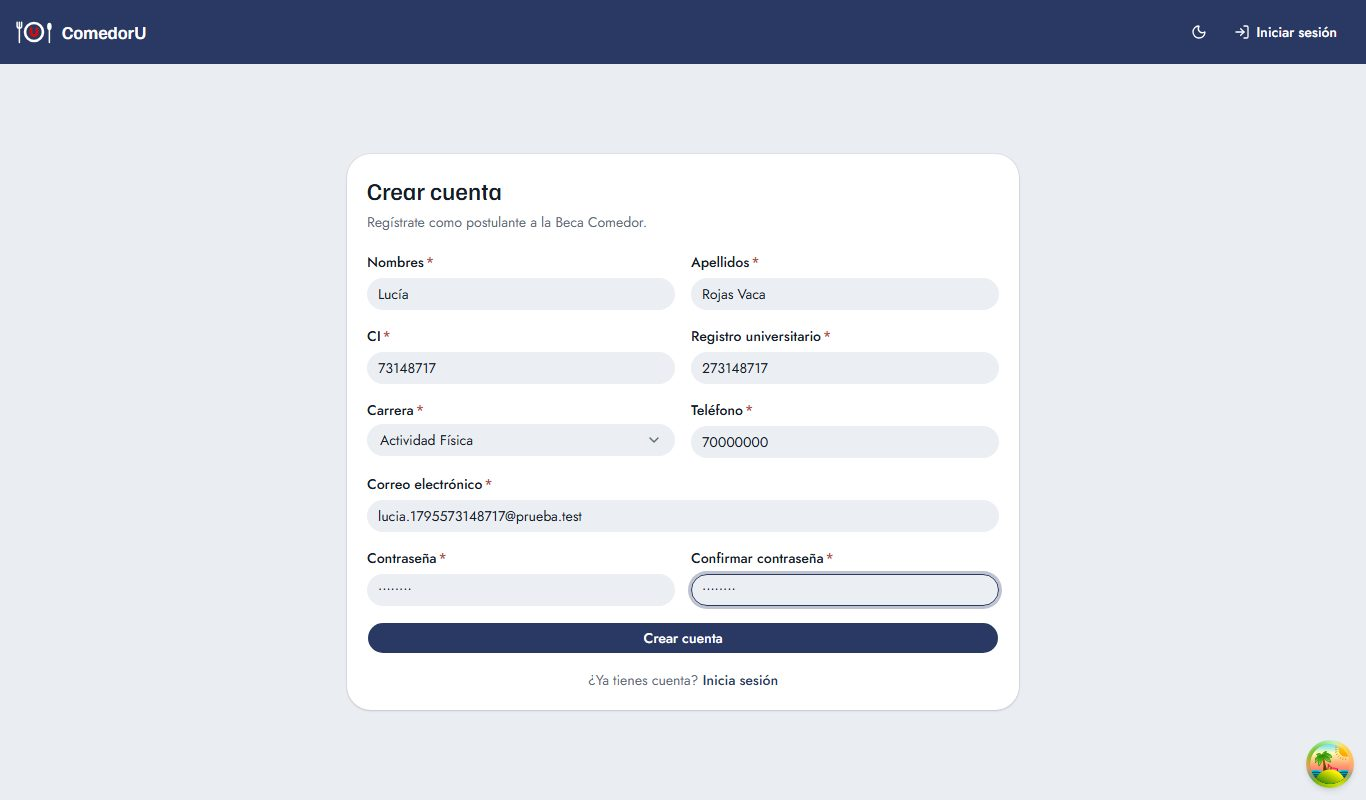
\includegraphics[width=0.93\linewidth,height=4.8cm,keepaspectratio]{images/154_CN_CU-01_A_inicial.jpg}}\vspace{2pt}\end{minipage}} \\
Pasos & {1. Abrir \texttt{/\allowbreak{}registro}.\newline 2. Completar todos los campos del formulario.\newline 3. Pulsar «Crear cuenta».} \\
Resultado esperado & {Se crea la cuenta con rol Postulante, se abre la sesión y se muestra el panel del postulante.} \\
Resultado obtenido & {La cuenta se creó y la aplicación quedó en \texttt{/\allowbreak{}panel} con el saludo «Hola, Lucía» y la convocatoria abierta con el botón «Postular ahora».} \\
Captura de imagen final & {\begin{minipage}[t]{\linewidth}\strut\par\vspace{3pt}\fcolorbox{gray}{white}{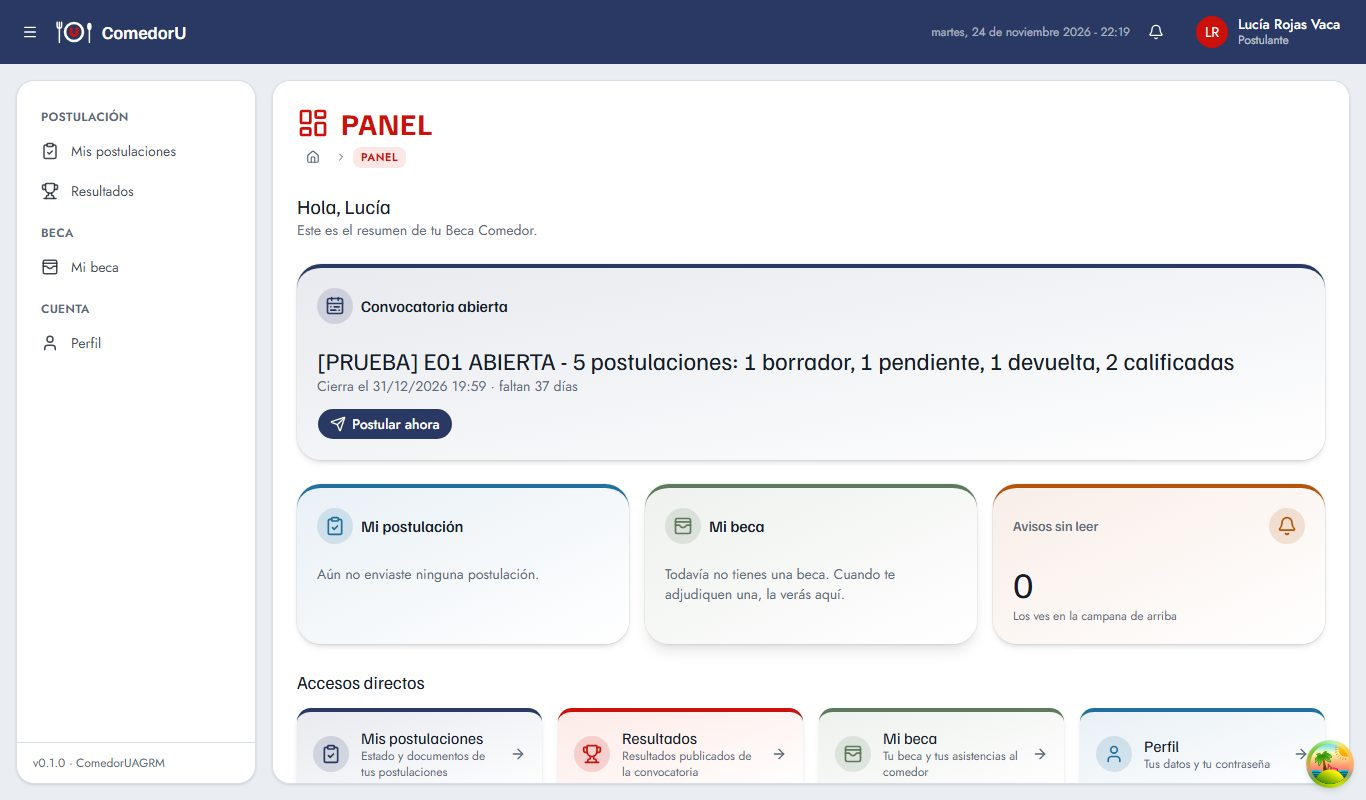
\includegraphics[width=0.93\linewidth,height=4.8cm,keepaspectratio]{images/155_CN_CU-01_A_final.jpg}}\vspace{2pt}\end{minipage}} \\
Resultado de prueba & {\textcolor{green!45!black}{\textbf{CORRECTO}}} \\
\end{longtable}
\endgroup
\addtocounter{table}{-1}
\vspace{-0.5\baselineskip}

\refstepcounter{table}\label{tab:cn_cu01_b}
\addcontentsline{lot}{table}{\protect\numberline{\thetable}CU-01. Registrarse y autenticarse (credenciales inválidas)}
\noindent\textbf{Tabla~\thetable}\par\nopagebreak
\noindent\textit{CU-01. Registrarse y autenticarse (credenciales inválidas)}\par\nopagebreak
\begingroup\footnotesize\linespread{1}\selectfont
\setlength{\LTleft}{0pt}\setlength{\LTright}{\fill}
\begin{longtable}{>{\raggedright\arraybackslash}p{3.6cm} >{\raggedright\arraybackslash}p{11.4cm}}
\toprule
\textbf{Campo} & \textbf{Contenido} \\
\midrule
\endfirsthead
\toprule
\textbf{Campo} & \textbf{Contenido} \\
\midrule
\endhead
\midrule
\multicolumn{2}{r}{\textit{Continúa en la siguiente página}} \\
\endfoot
\bottomrule
\multicolumn{2}{l}{\textit{Nota.} Elaboración propia a partir de la ejecución de la prueba.} \\
\endlastfoot
Nombre del caso de prueba & {CU-01. Registrarse y autenticarse (credenciales inválidas)} \\
Descripción & {El sistema rechaza el acceso cuando la contraseña no corresponde, sin revelar cuál dato falló.} \\
Precondición & {Existe la cuenta \texttt{admin@\allowbreak{}dubss.\allowbreak{}com}.} \\
Datos de entrada & {Correo \texttt{admin@\allowbreak{}dubss.\allowbreak{}com}, contraseña «incorrecta1».} \\
Condición de ejecución & {No aplica} \\
Captura de imagen inicial & {\begin{minipage}[t]{\linewidth}\strut\par\vspace{3pt}\fcolorbox{gray}{white}{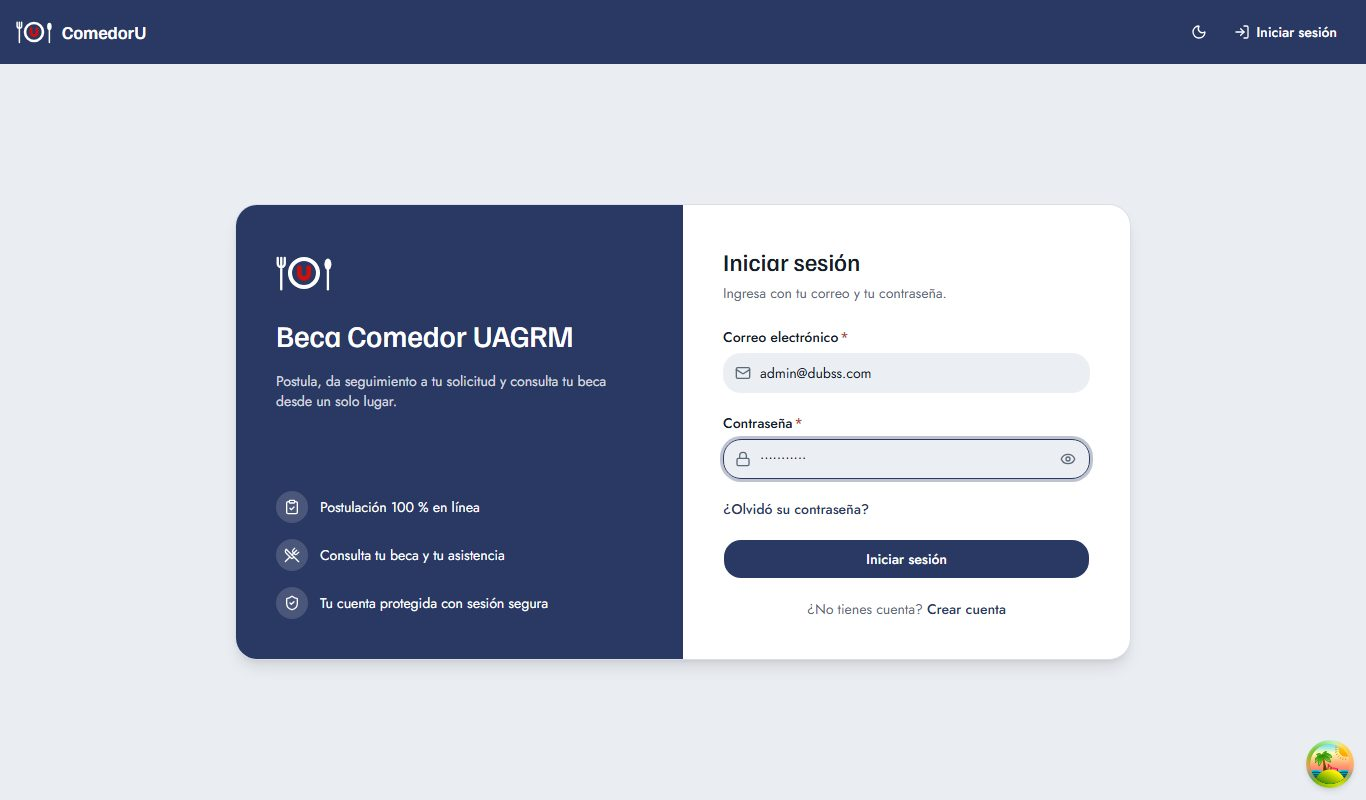
\includegraphics[width=0.93\linewidth,height=4.8cm,keepaspectratio]{images/156_CN_CU-01_B_inicial.jpg}}\vspace{2pt}\end{minipage}} \\
Pasos & {1. Abrir \texttt{/\allowbreak{}login}.\newline 2. Escribir el correo y la contraseña incorrecta.\newline 3. Pulsar «Iniciar sesión».} \\
Resultado esperado & {No se abre la sesión y se muestra un mensaje genérico de credenciales incorrectas.} \\
Resultado obtenido & {Se permaneció en \texttt{/\allowbreak{}login} y apareció el mensaje «Correo o contraseña incorrectos.».} \\
Captura de imagen final & {\begin{minipage}[t]{\linewidth}\strut\par\vspace{3pt}\fcolorbox{gray}{white}{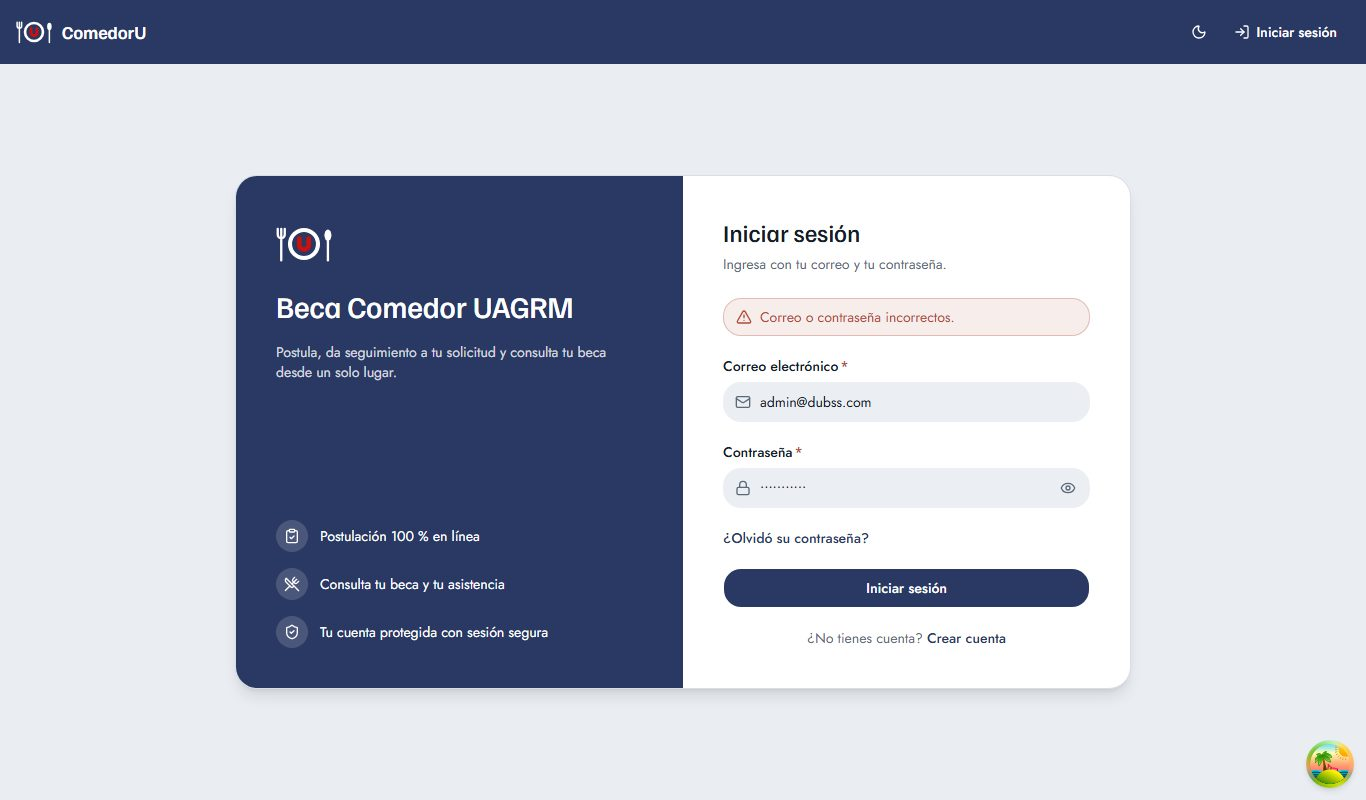
\includegraphics[width=0.93\linewidth,height=4.8cm,keepaspectratio]{images/157_CN_CU-01_B_final.jpg}}\vspace{2pt}\end{minipage}} \\
Resultado de prueba & {\textcolor{green!45!black}{\textbf{CORRECTO}}} \\
\end{longtable}
\endgroup
\addtocounter{table}{-1}
\vspace{-0.5\baselineskip}

\refstepcounter{table}\label{tab:cn_cu01_c}
\addcontentsline{lot}{table}{\protect\numberline{\thetable}CU-01. Registrarse y autenticarse (inicio de sesión)}
\noindent\textbf{Tabla~\thetable}\par\nopagebreak
\noindent\textit{CU-01. Registrarse y autenticarse (inicio de sesión)}\par\nopagebreak
\begingroup\footnotesize\linespread{1}\selectfont
\setlength{\LTleft}{0pt}\setlength{\LTright}{\fill}
\begin{longtable}{>{\raggedright\arraybackslash}p{3.6cm} >{\raggedright\arraybackslash}p{11.4cm}}
\toprule
\textbf{Campo} & \textbf{Contenido} \\
\midrule
\endfirsthead
\toprule
\textbf{Campo} & \textbf{Contenido} \\
\midrule
\endhead
\midrule
\multicolumn{2}{r}{\textit{Continúa en la siguiente página}} \\
\endfoot
\bottomrule
\multicolumn{2}{l}{\textit{Nota.} Elaboración propia a partir de la ejecución de la prueba.} \\
\endlastfoot
Nombre del caso de prueba & {CU-01. Registrarse y autenticarse (inicio de sesión)} \\
Descripción & {Con credenciales válidas el sistema abre la sesión y redirige al módulo del rol.} \\
Precondición & {Existe la cuenta del Administrador DUBSS sembrada (\texttt{admin@\allowbreak{}dubss.\allowbreak{}com}).} \\
Datos de entrada & {Correo \texttt{admin@\allowbreak{}dubss.\allowbreak{}com}, contraseña de desarrollo.} \\
Condición de ejecución & {No aplica} \\
Captura de imagen inicial & {\begin{minipage}[t]{\linewidth}\strut\par\vspace{3pt}\fcolorbox{gray}{white}{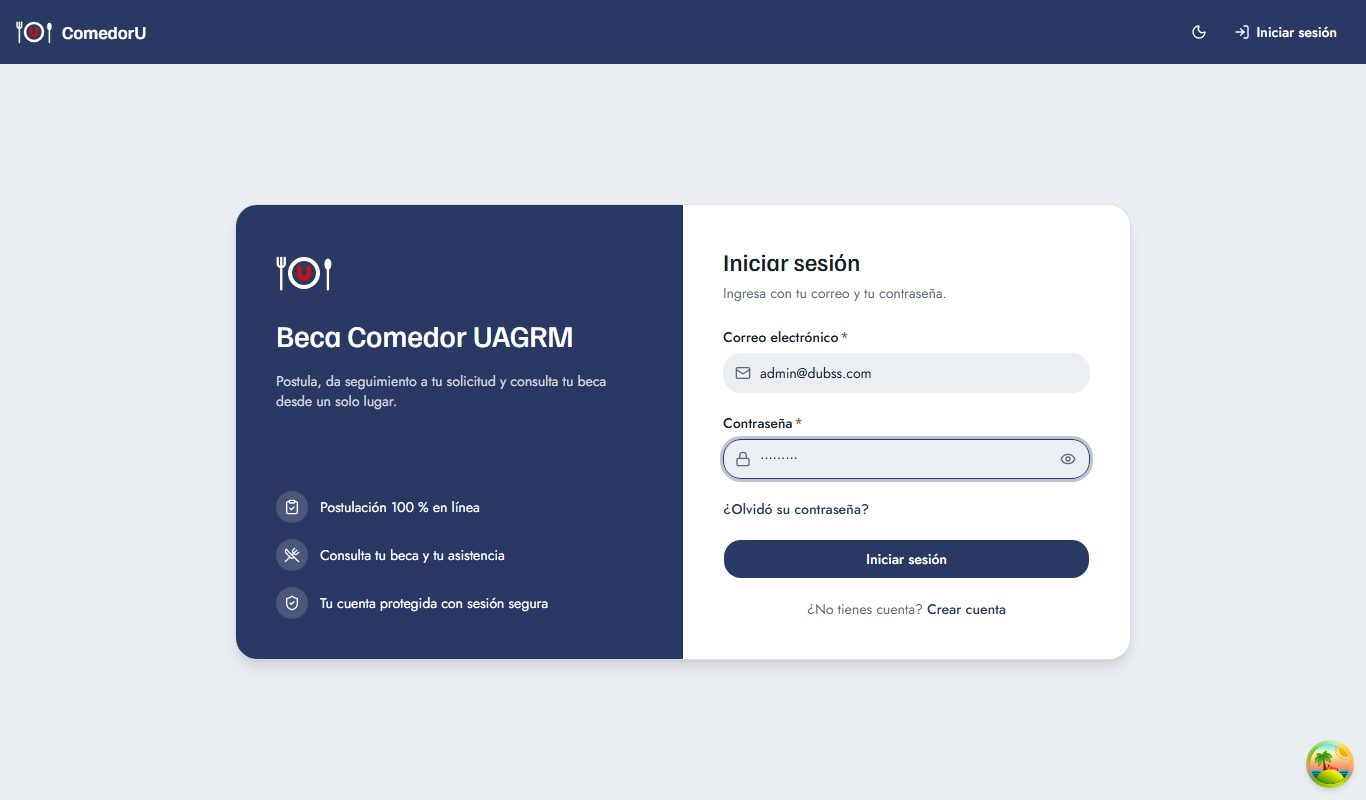
\includegraphics[width=0.93\linewidth,height=4.8cm,keepaspectratio]{images/158_CN_CU-01_C_inicial.jpg}}\vspace{2pt}\end{minipage}} \\
Pasos & {1. Abrir \texttt{/\allowbreak{}login}.\newline 2. Escribir las credenciales.\newline 3. Pulsar «Iniciar sesión».} \\
Resultado esperado & {Se abre la sesión y se muestra el panel del administrador.} \\
Resultado obtenido & {La aplicación redirigió a \texttt{/\allowbreak{}panel} con el panel del administrador.} \\
Captura de imagen final & {\begin{minipage}[t]{\linewidth}\strut\par\vspace{3pt}\fcolorbox{gray}{white}{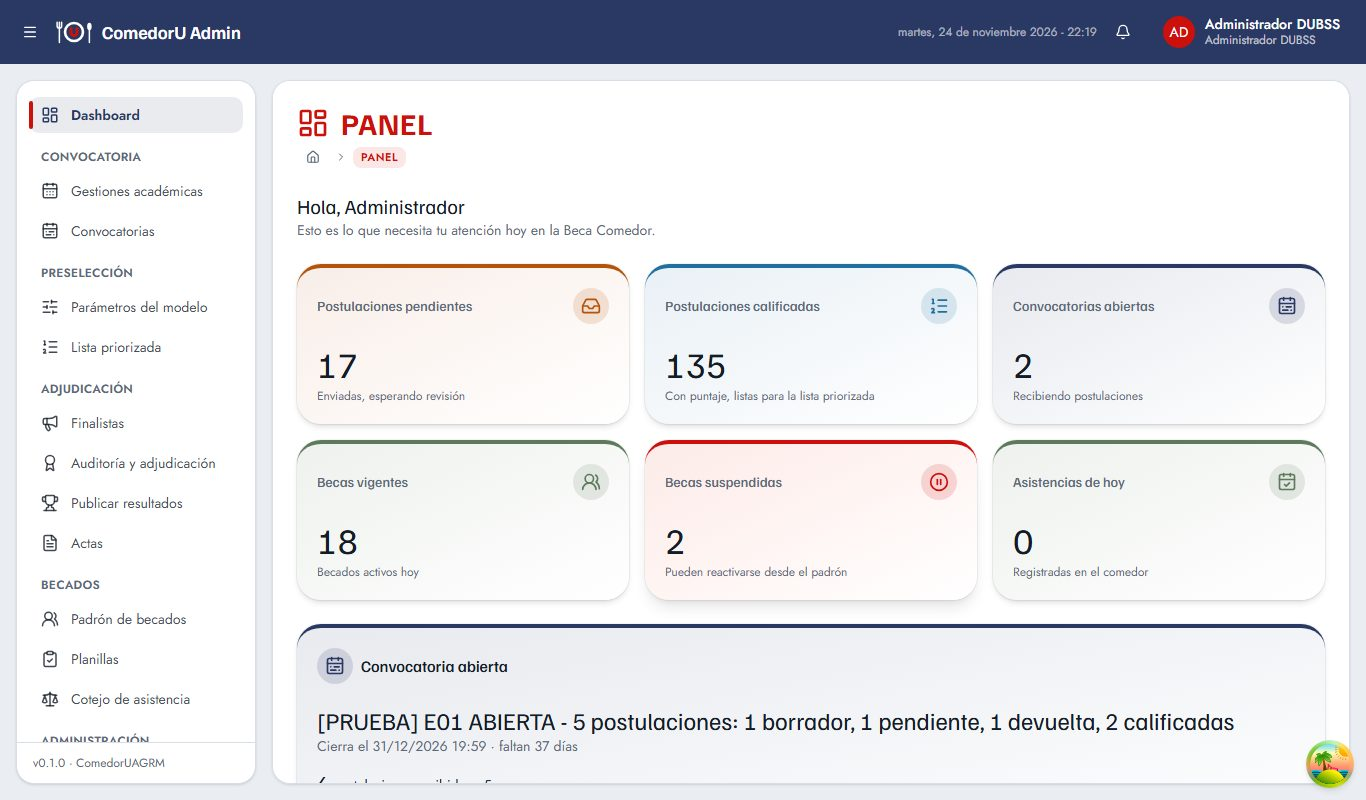
\includegraphics[width=0.93\linewidth,height=4.8cm,keepaspectratio]{images/159_CN_CU-01_C_final.jpg}}\vspace{2pt}\end{minipage}} \\
Resultado de prueba & {\textcolor{green!45!black}{\textbf{CORRECTO}}} \\
\end{longtable}
\endgroup
\addtocounter{table}{-1}
\vspace{-0.5\baselineskip}

\refstepcounter{table}\label{tab:cn_cu01_d}
\addcontentsline{lot}{table}{\protect\numberline{\thetable}CU-01. Registrarse y autenticarse (redirección por rol)}
\noindent\textbf{Tabla~\thetable}\par\nopagebreak
\noindent\textit{CU-01. Registrarse y autenticarse (redirección por rol)}\par\nopagebreak
\begingroup\footnotesize\linespread{1}\selectfont
\setlength{\LTleft}{0pt}\setlength{\LTright}{\fill}
\begin{longtable}{>{\raggedright\arraybackslash}p{3.6cm} >{\raggedright\arraybackslash}p{11.4cm}}
\toprule
\textbf{Campo} & \textbf{Contenido} \\
\midrule
\endfirsthead
\toprule
\textbf{Campo} & \textbf{Contenido} \\
\midrule
\endhead
\midrule
\multicolumn{2}{r}{\textit{Continúa en la siguiente página}} \\
\endfoot
\bottomrule
\multicolumn{2}{l}{\textit{Nota.} Elaboración propia a partir de la ejecución de la prueba.} \\
\endlastfoot
Nombre del caso de prueba & {CU-01. Registrarse y autenticarse (redirección por rol)} \\
Descripción & {Cada rol llega a su propio módulo después de iniciar sesión.} \\
Precondición & {Existe la cuenta \texttt{directivo@\allowbreak{}dubss.\allowbreak{}com}.} \\
Datos de entrada & {Correo \texttt{directivo@\allowbreak{}dubss.\allowbreak{}com}, contraseña de desarrollo.} \\
Condición de ejecución & {No aplica} \\
Captura de imagen inicial & {No aplica: la prueba comprueba un estado y no tiene pantalla previa distinta de la final.} \\
Pasos & {1. Abrir \texttt{/\allowbreak{}login}.\newline 2. Escribir las credenciales del directivo.\newline 3. Pulsar «Iniciar sesión».} \\
Resultado esperado & {El directivo llega a su dashboard.} \\
Resultado obtenido & {La aplicación redirigió a \texttt{/\allowbreak{}dashboard} (menú con solo «Dashboard»).} \\
Captura de imagen final & {\begin{minipage}[t]{\linewidth}\strut\par\vspace{3pt}\fcolorbox{gray}{white}{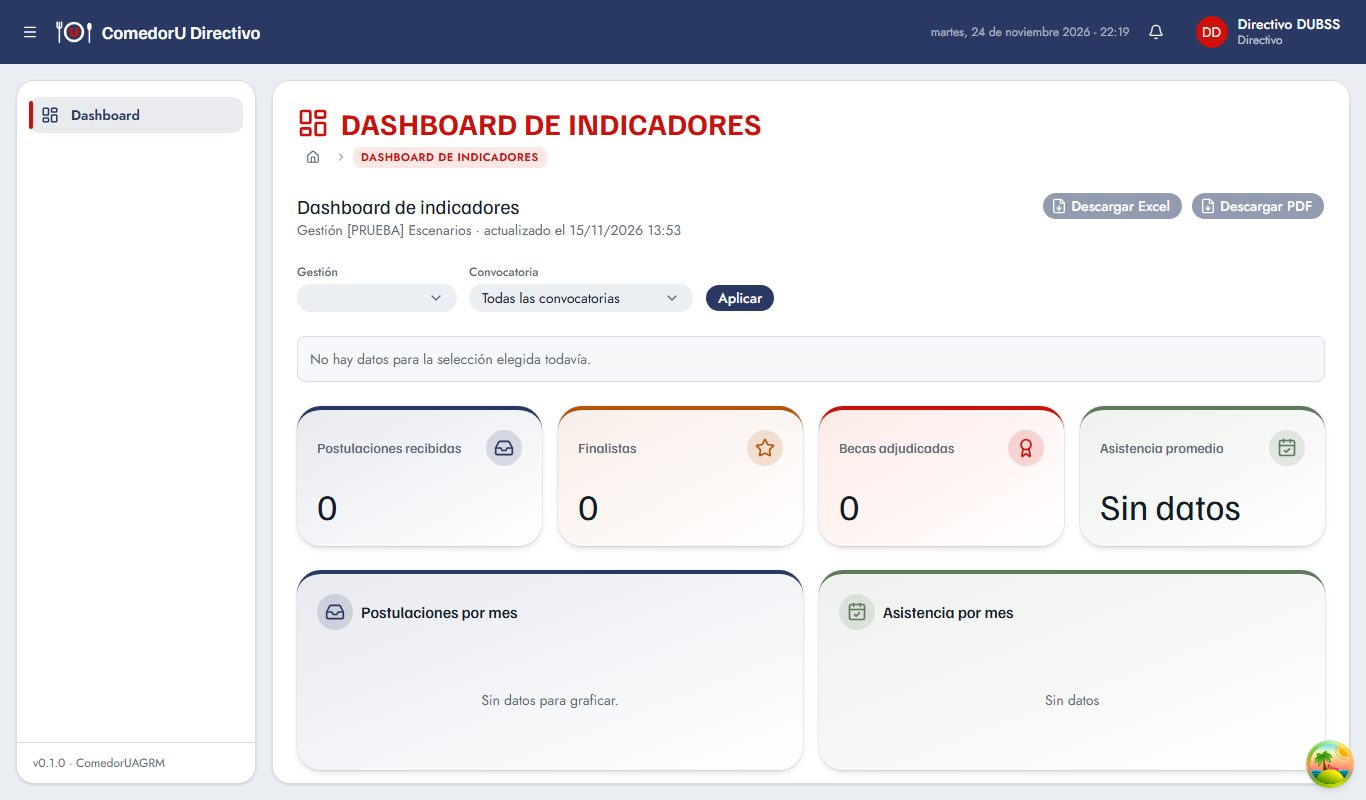
\includegraphics[width=0.93\linewidth,height=4.8cm,keepaspectratio]{images/160_CN_CU-01_D_directivo.jpg}}\vspace{2pt}\end{minipage}} \\
Resultado de prueba & {\textcolor{green!45!black}{\textbf{CORRECTO}}} \\
\end{longtable}
\endgroup
\addtocounter{table}{-1}
\vspace{-0.5\baselineskip}

\paragraph{CU-04. Consultar estado de postulación.}\label{sec:cn_cu04} 

\refstepcounter{table}\label{tab:cn_cu04_a}
\addcontentsline{lot}{table}{\protect\numberline{\thetable}CU-04. Consultar estado de postulación (lista y detalle)}
\noindent\textbf{Tabla~\thetable}\par\nopagebreak
\noindent\textit{CU-04. Consultar estado de postulación (lista y detalle)}\par\nopagebreak
\begingroup\footnotesize\linespread{1}\selectfont
\setlength{\LTleft}{0pt}\setlength{\LTright}{\fill}
\begin{longtable}{>{\raggedright\arraybackslash}p{3.6cm} >{\raggedright\arraybackslash}p{11.4cm}}
\toprule
\textbf{Campo} & \textbf{Contenido} \\
\midrule
\endfirsthead
\toprule
\textbf{Campo} & \textbf{Contenido} \\
\midrule
\endhead
\midrule
\multicolumn{2}{r}{\textit{Continúa en la siguiente página}} \\
\endfoot
\bottomrule
\multicolumn{2}{l}{\textit{Nota.} Elaboración propia a partir de la ejecución de la prueba.} \\
\endlastfoot
Nombre del caso de prueba & {CU-04. Consultar estado de postulación (lista y detalle)} \\
Descripción & {El postulante ve sus postulaciones enviadas con su estado y el recorrido de cada una.} \\
Precondición & {Sesión de \texttt{postulante.\allowbreak{}finalista@\allowbreak{}prueba.\allowbreak{}local} con postulaciones sembradas en varios estados.} \\
Datos de entrada & {Ninguno.} \\
Condición de ejecución & {No aplica} \\
Captura de imagen inicial & {\begin{minipage}[t]{\linewidth}\strut\par\vspace{3pt}\fcolorbox{gray}{white}{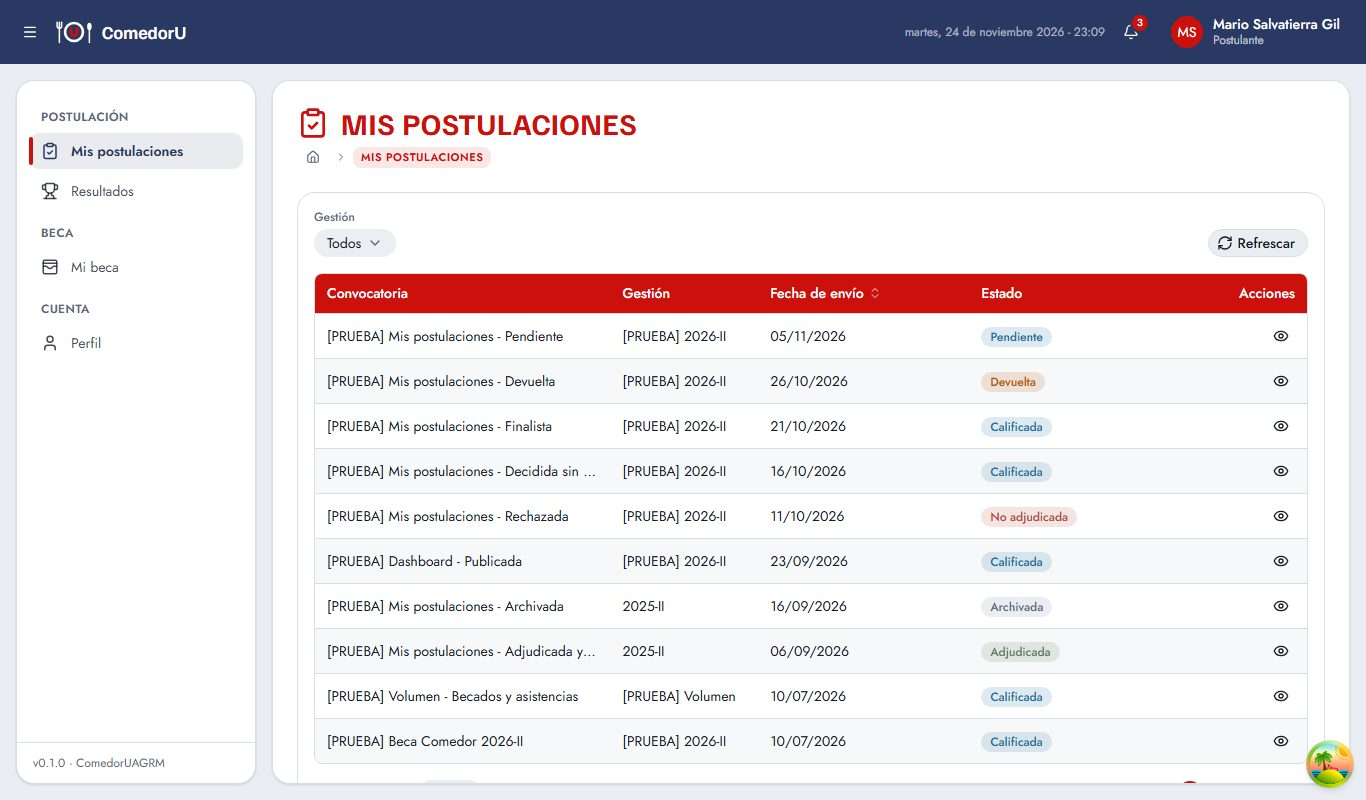
\includegraphics[width=0.93\linewidth,height=4.8cm,keepaspectratio]{images/161_CN_CU-04_A_inicial.jpg}}\vspace{2pt}\end{minipage}} \\
Pasos & {1. Abrir «Mis postulaciones».\newline 2. Pulsar «Ver» en la primera postulación.} \\
Resultado esperado & {La lista muestra convocatoria, gestión, fecha de envío y estado; el detalle muestra el recorrido de la postulación.} \\
Resultado obtenido & {La lista mostró las postulaciones de más reciente a más antigua (Pendiente, Devuelta, Calificada, No adjudicada…). El detalle de «Mis postulaciones - Pendiente» mostró «Recorrido de tu postulación» con «Postulación enviada 05/11/2026».} \\
Captura de imagen final & {\begin{minipage}[t]{\linewidth}\strut\par\vspace{3pt}\fcolorbox{gray}{white}{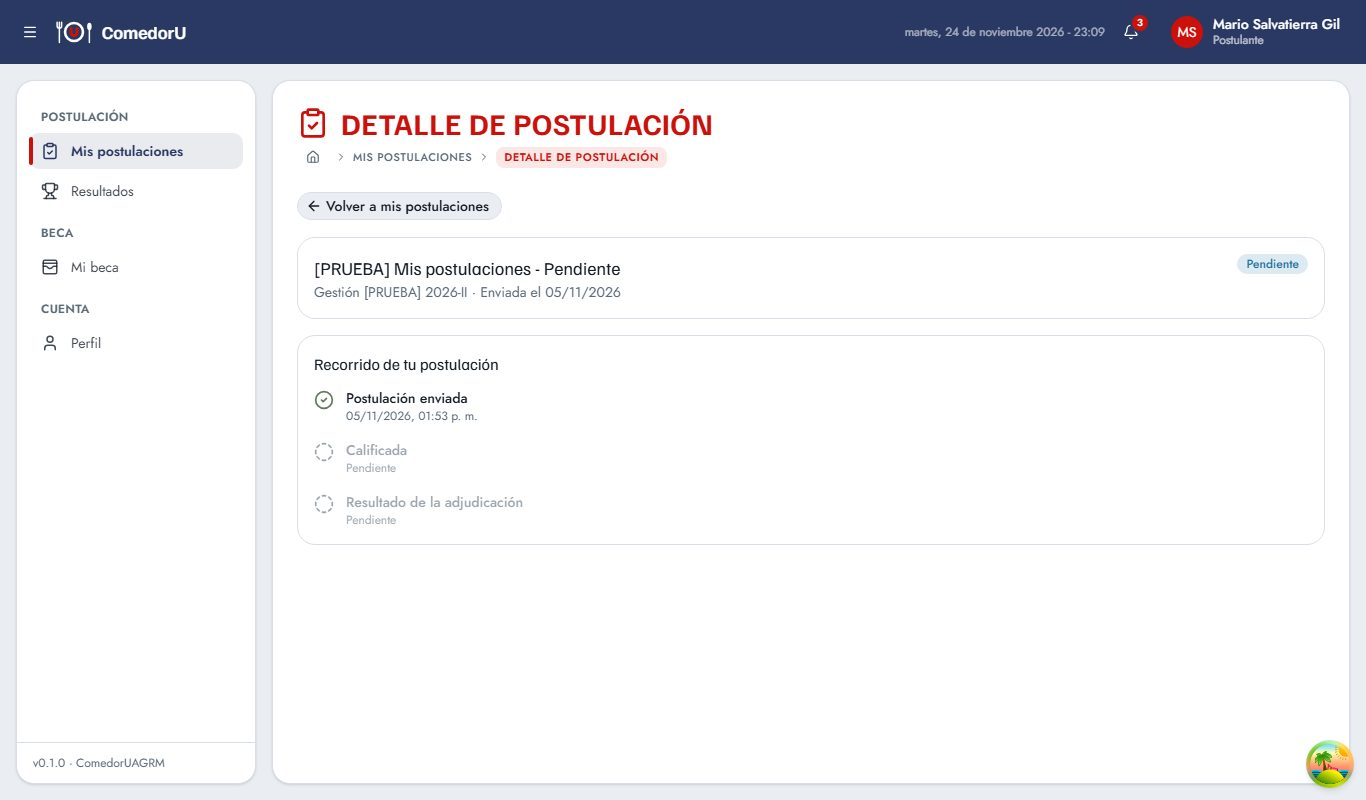
\includegraphics[width=0.93\linewidth,height=4.8cm,keepaspectratio]{images/162_CN_CU-04_A_final.jpg}}\vspace{2pt}\end{minipage}} \\
Resultado de prueba & {\textcolor{green!45!black}{\textbf{CORRECTO}}} \\
\end{longtable}
\endgroup
\addtocounter{table}{-1}
\vspace{-0.5\baselineskip}

\refstepcounter{table}\label{tab:cn_cu04_b}
\addcontentsline{lot}{table}{\protect\numberline{\thetable}CU-04. Consultar estado de postulación (sin postulaciones)}
\noindent\textbf{Tabla~\thetable}\par\nopagebreak
\noindent\textit{CU-04. Consultar estado de postulación (sin postulaciones)}\par\nopagebreak
\begingroup\footnotesize\linespread{1}\selectfont
\setlength{\LTleft}{0pt}\setlength{\LTright}{\fill}
\begin{longtable}{>{\raggedright\arraybackslash}p{3.6cm} >{\raggedright\arraybackslash}p{11.4cm}}
\toprule
\textbf{Campo} & \textbf{Contenido} \\
\midrule
\endfirsthead
\toprule
\textbf{Campo} & \textbf{Contenido} \\
\midrule
\endhead
\midrule
\multicolumn{2}{r}{\textit{Continúa en la siguiente página}} \\
\endfoot
\bottomrule
\multicolumn{2}{l}{\textit{Nota.} Elaboración propia a partir de la ejecución de la prueba.} \\
\endlastfoot
Nombre del caso de prueba & {CU-04. Consultar estado de postulación (sin postulaciones)} \\
Descripción & {Si no hay postulaciones enviadas, el sistema lo informa.} \\
Precondición & {Cuenta de postulante recién creada.} \\
Datos de entrada & {Ninguno.} \\
Condición de ejecución & {No aplica} \\
Captura de imagen inicial & {No aplica: la prueba comprueba un estado y no tiene pantalla previa distinta de la final.} \\
Pasos & {1. Abrir «Mis postulaciones».} \\
Resultado esperado & {Mensaje informativo con la opción de postular.} \\
Resultado obtenido & {Se mostró «Todavía no enviaste ninguna postulación» y el botón «Postular».} \\
Captura de imagen final & {\begin{minipage}[t]{\linewidth}\strut\par\vspace{3pt}\fcolorbox{gray}{white}{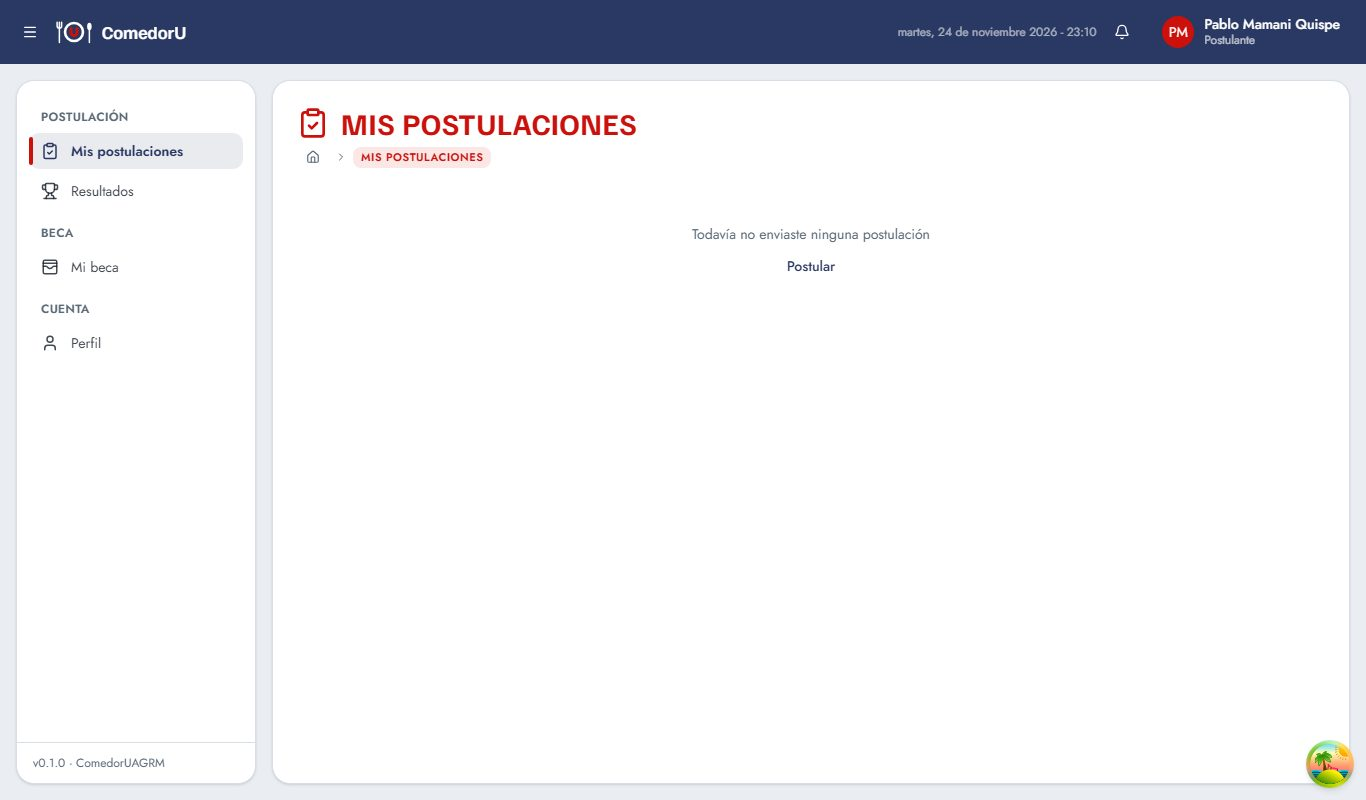
\includegraphics[width=0.93\linewidth,height=4.8cm,keepaspectratio]{images/163_CN_CU-04_B_final.jpg}}\vspace{2pt}\end{minipage}} \\
Resultado de prueba & {\textcolor{green!45!black}{\textbf{CORRECTO}}} \\
\end{longtable}
\endgroup
\addtocounter{table}{-1}
\vspace{-0.5\baselineskip}

\paragraph{CU-05. Auditar y adjudicar becas.}\label{sec:cn_cu05} 

\refstepcounter{table}\label{tab:cn_cu05_a}
\addcontentsline{lot}{table}{\protect\numberline{\thetable}CU-05. Auditar y adjudicar becas (adjudicación)}
\noindent\textbf{Tabla~\thetable}\par\nopagebreak
\noindent\textit{CU-05. Auditar y adjudicar becas (adjudicación)}\par\nopagebreak
\begingroup\footnotesize\linespread{1}\selectfont
\setlength{\LTleft}{0pt}\setlength{\LTright}{\fill}
\begin{longtable}{>{\raggedright\arraybackslash}p{3.6cm} >{\raggedright\arraybackslash}p{11.4cm}}
\toprule
\textbf{Campo} & \textbf{Contenido} \\
\midrule
\endfirsthead
\toprule
\textbf{Campo} & \textbf{Contenido} \\
\midrule
\endhead
\midrule
\multicolumn{2}{r}{\textit{Continúa en la siguiente página}} \\
\endfoot
\bottomrule
\multicolumn{2}{l}{\textit{Nota.} Elaboración propia a partir de la ejecución de la prueba.} \\
\endlastfoot
Nombre del caso de prueba & {CU-05. Auditar y adjudicar becas (adjudicación)} \\
Descripción & {El administrador adjudica la beca al finalista validado, dentro de los cupos y sobre el puntaje mínimo.} \\
Precondición & {Convocatoria sembrada «[PRUEBA] E04»: 3 cupos, puntaje mínimo 40; finalista 1 (Elena Suárez Molina) validado.} \\
Datos de entrada & {Finalista 1 de E04; sin datos adicionales.} \\
Condición de ejecución & {El expediente debe estar auditado como «Validado», con puntaje total mayor o igual al mínimo y cupos libres.} \\
Captura de imagen inicial & {\begin{minipage}[t]{\linewidth}\strut\par\vspace{3pt}\fcolorbox{gray}{white}{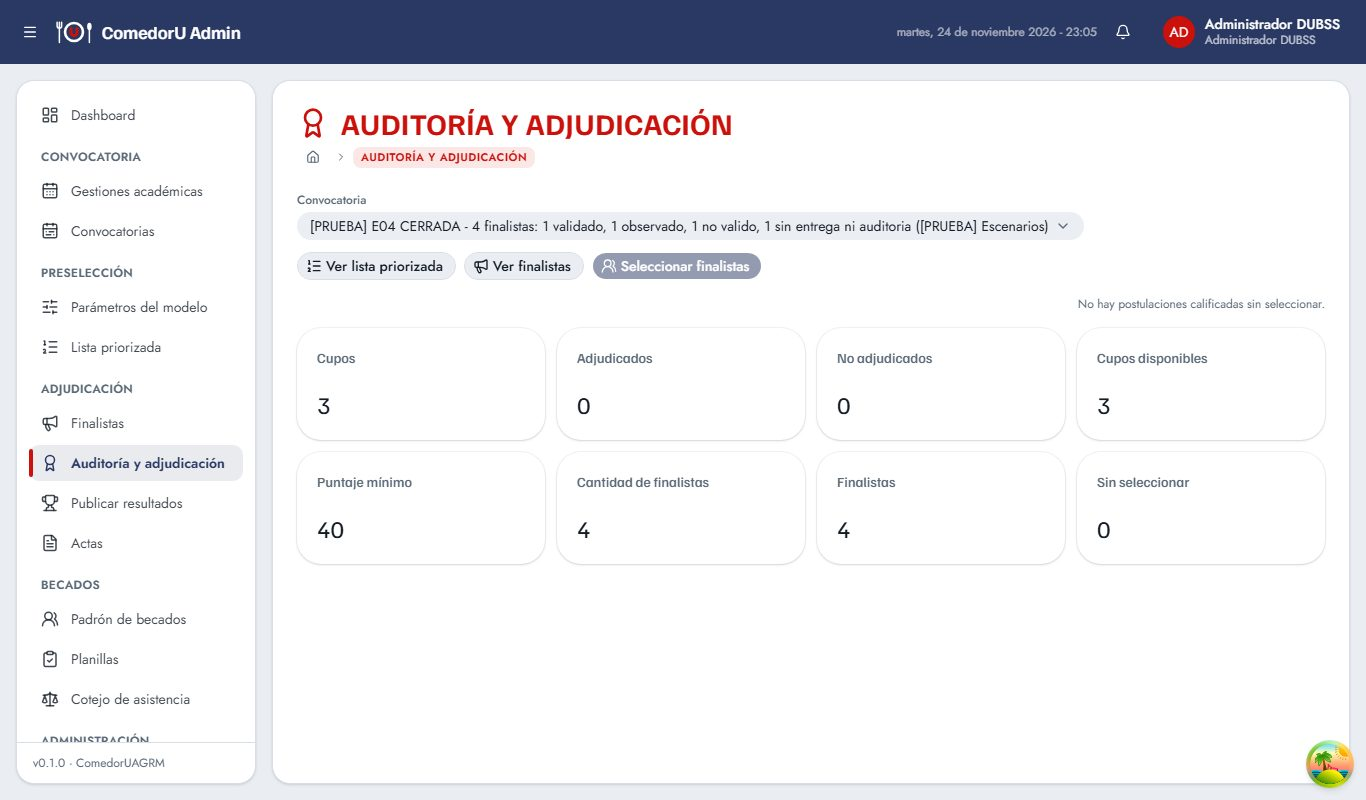
\includegraphics[width=0.93\linewidth,height=4.8cm,keepaspectratio]{images/164_CN_CU-05_A_inicial.jpg}}\vspace{2pt}\end{minipage}} \\
Pasos & {1. Abrir «Auditoría y adjudicación», elegir E04 y ver el panel.\newline 2. Abrir el expediente del finalista 1 y pulsar «Adjudicar».\newline 3. Revisar la ventana de confirmación y pulsar «Adjudicar».\newline 4. Volver al panel de E04.} \\
Resultado esperado & {La postulación queda «adjudicada» y los cupos disponibles bajan en uno.} \\
Resultado obtenido & {Antes: cupos 3, adjudicados 0, disponibles 3. La ventana mostró puntaje total 95,00, cupos disponibles 3, mínimo 40,00. Después: estado «adjudicada», adjudicados 1 y cupos disponibles 2.} \\
Captura de imagen final & {\begin{minipage}[t]{\linewidth}\strut\par\vspace{3pt}\fcolorbox{gray}{white}{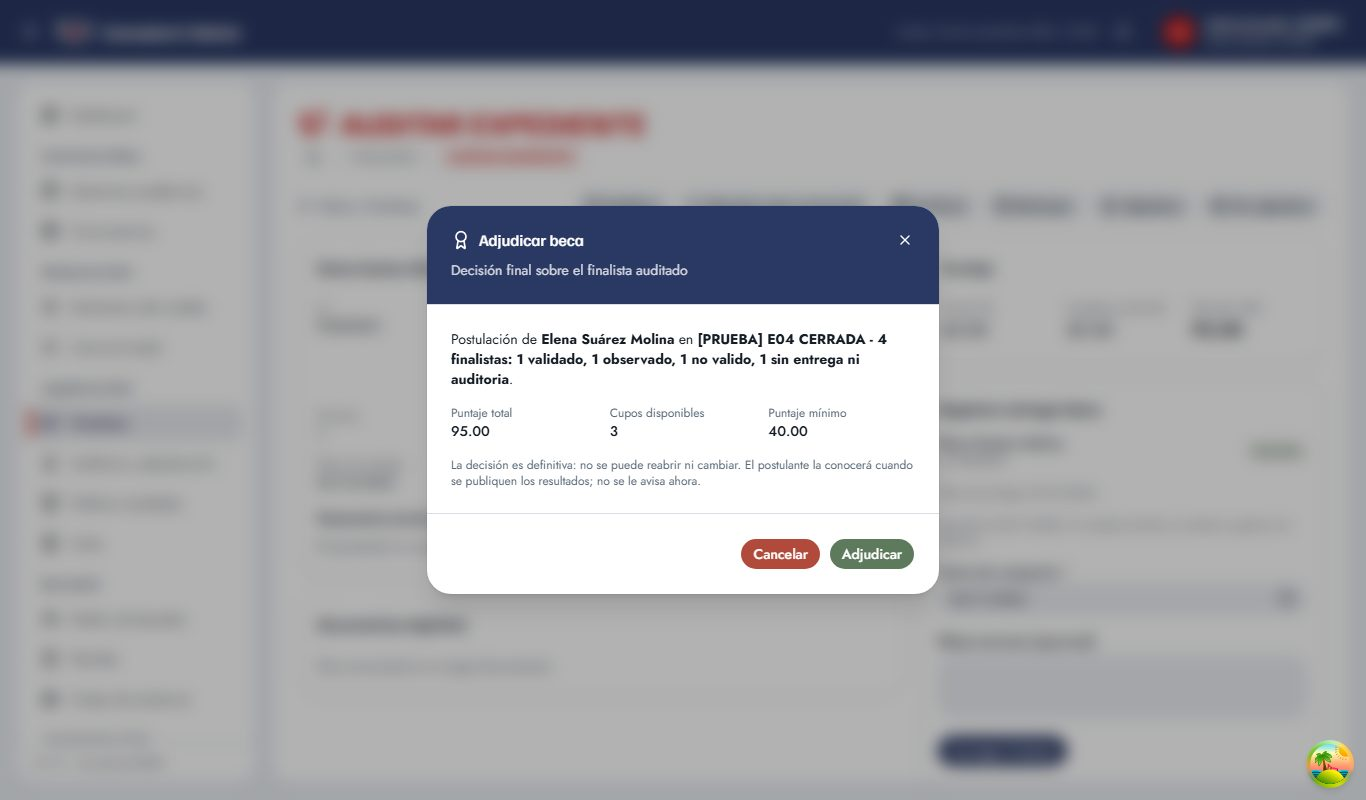
\includegraphics[width=0.93\linewidth,height=4.8cm,keepaspectratio]{images/165_CN_CU-05_A_confirmacion.jpg}}\vspace{2pt}\par\vspace{3pt}\fcolorbox{gray}{white}{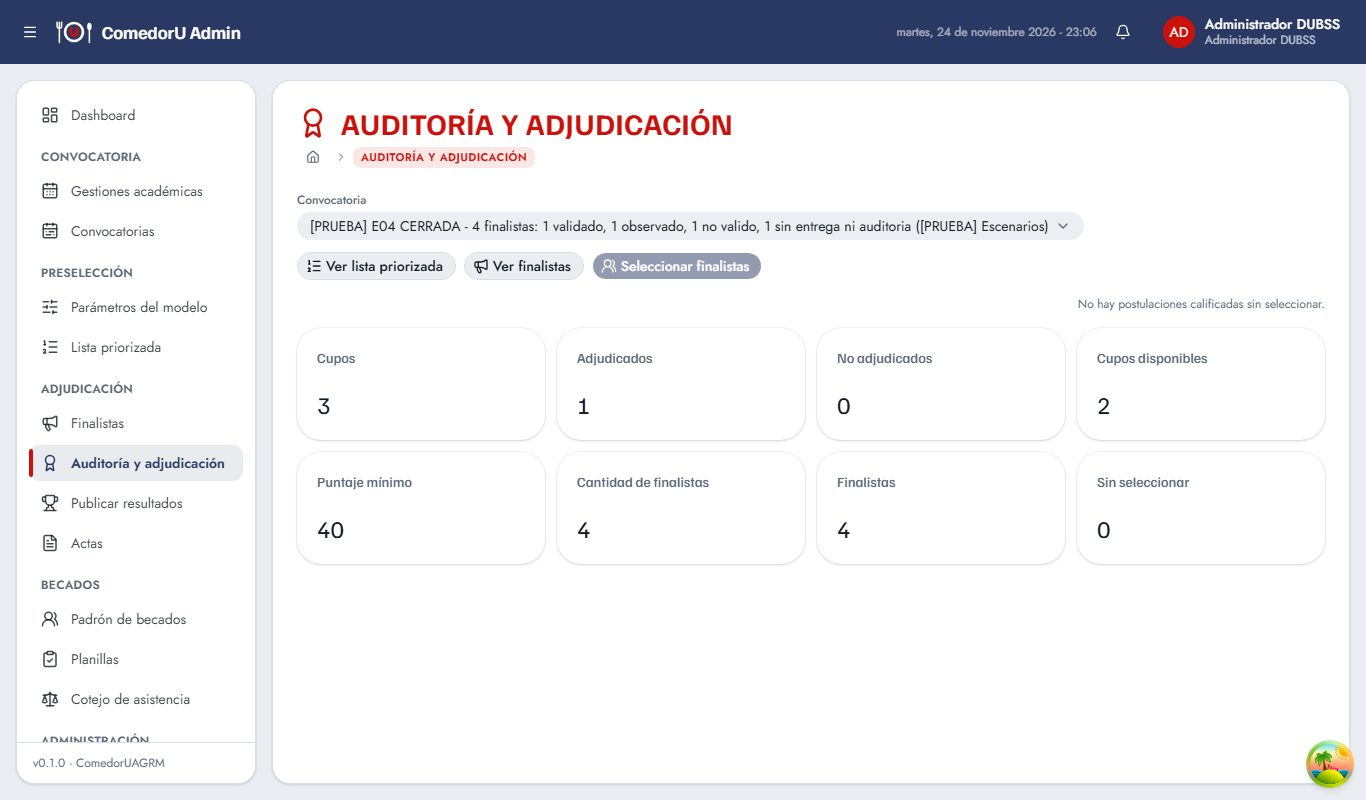
\includegraphics[width=0.93\linewidth,height=4.8cm,keepaspectratio]{images/166_CN_CU-05_A_final.jpg}}\vspace{2pt}\end{minipage}} \\
Resultado de prueba & {\textcolor{green!45!black}{\textbf{CORRECTO}}} \\
\end{longtable}
\endgroup
\addtocounter{table}{-1}
\vspace{-0.5\baselineskip}

\refstepcounter{table}\label{tab:cn_cu05_b}
\addcontentsline{lot}{table}{\protect\numberline{\thetable}CU-05. Auditar y adjudicar becas (sin auditoría)}
\noindent\textbf{Tabla~\thetable}\par\nopagebreak
\noindent\textit{CU-05. Auditar y adjudicar becas (sin auditoría)}\par\nopagebreak
\begingroup\footnotesize\linespread{1}\selectfont
\setlength{\LTleft}{0pt}\setlength{\LTright}{\fill}
\begin{longtable}{>{\raggedright\arraybackslash}p{3.6cm} >{\raggedright\arraybackslash}p{11.4cm}}
\toprule
\textbf{Campo} & \textbf{Contenido} \\
\midrule
\endfirsthead
\toprule
\textbf{Campo} & \textbf{Contenido} \\
\midrule
\endhead
\midrule
\multicolumn{2}{r}{\textit{Continúa en la siguiente página}} \\
\endfoot
\bottomrule
\multicolumn{2}{l}{\textit{Nota.} Elaboración propia a partir de la ejecución de la prueba.} \\
\endlastfoot
Nombre del caso de prueba & {CU-05. Auditar y adjudicar becas (sin auditoría)} \\
Descripción & {No se puede decidir sobre un finalista sin auditoría.} \\
Precondición & {Finalista 4 de E04 sin entrega ni auditoría.} \\
Datos de entrada & {Expediente del finalista 4.} \\
Condición de ejecución & {No aplica} \\
Captura de imagen inicial & {\begin{minipage}[t]{\linewidth}\strut\par\vspace{3pt}\fcolorbox{gray}{white}{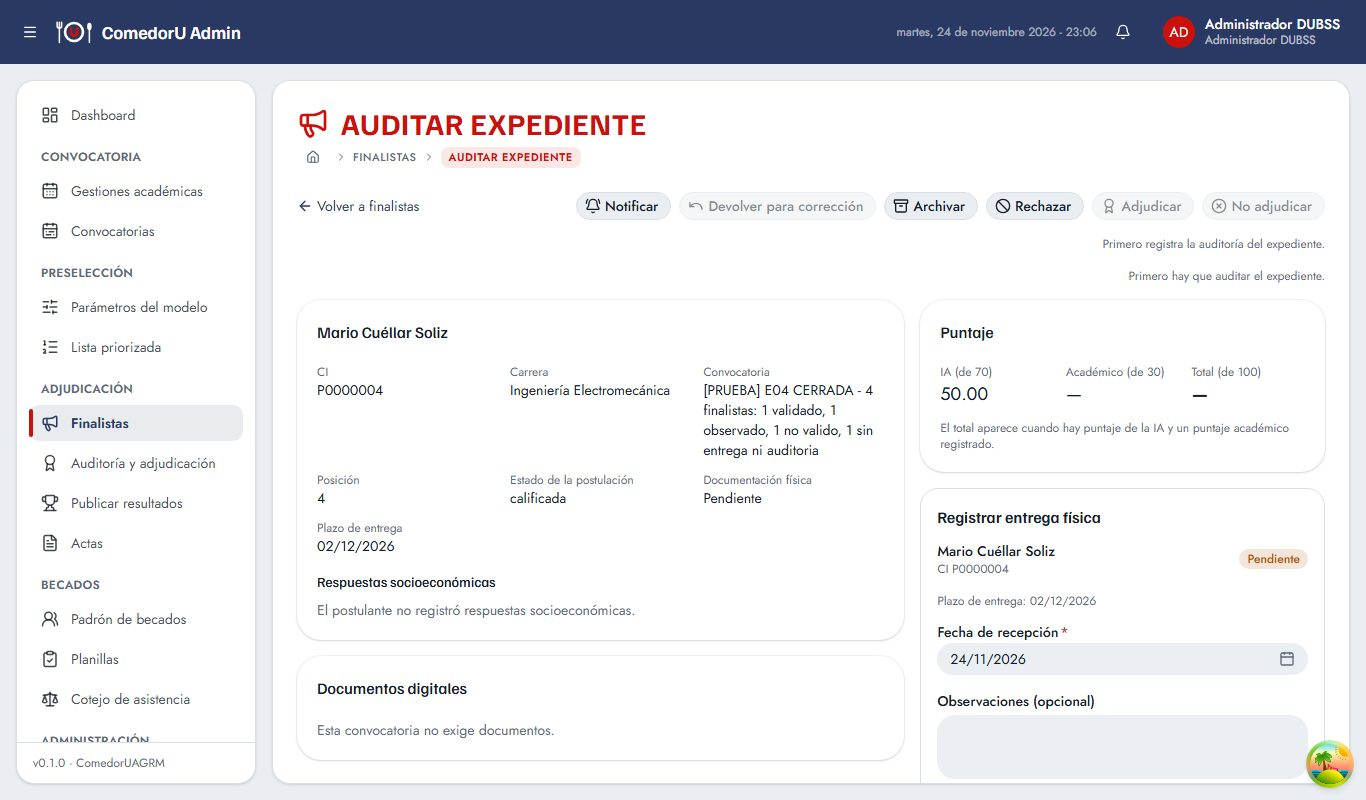
\includegraphics[width=0.93\linewidth,height=4.8cm,keepaspectratio]{images/167_CN_CU-05_B_inicial.jpg}}\vspace{2pt}\end{minipage}} \\
Pasos & {1. Abrir el expediente del finalista 4 de E04.\newline 2. Intentar pulsar «Adjudicar» y «No adjudicar».} \\
Resultado esperado & {Las dos decisiones no están disponibles y se pide auditar primero.} \\
Resultado obtenido & {Los botones «Adjudicar» y «No adjudicar» estaban deshabilitados con los avisos «Primero registra la auditoría del expediente.» y «Primero hay que auditar el expediente.».} \\
Captura de imagen final & {\begin{minipage}[t]{\linewidth}\strut\par\vspace{3pt}\fcolorbox{gray}{white}{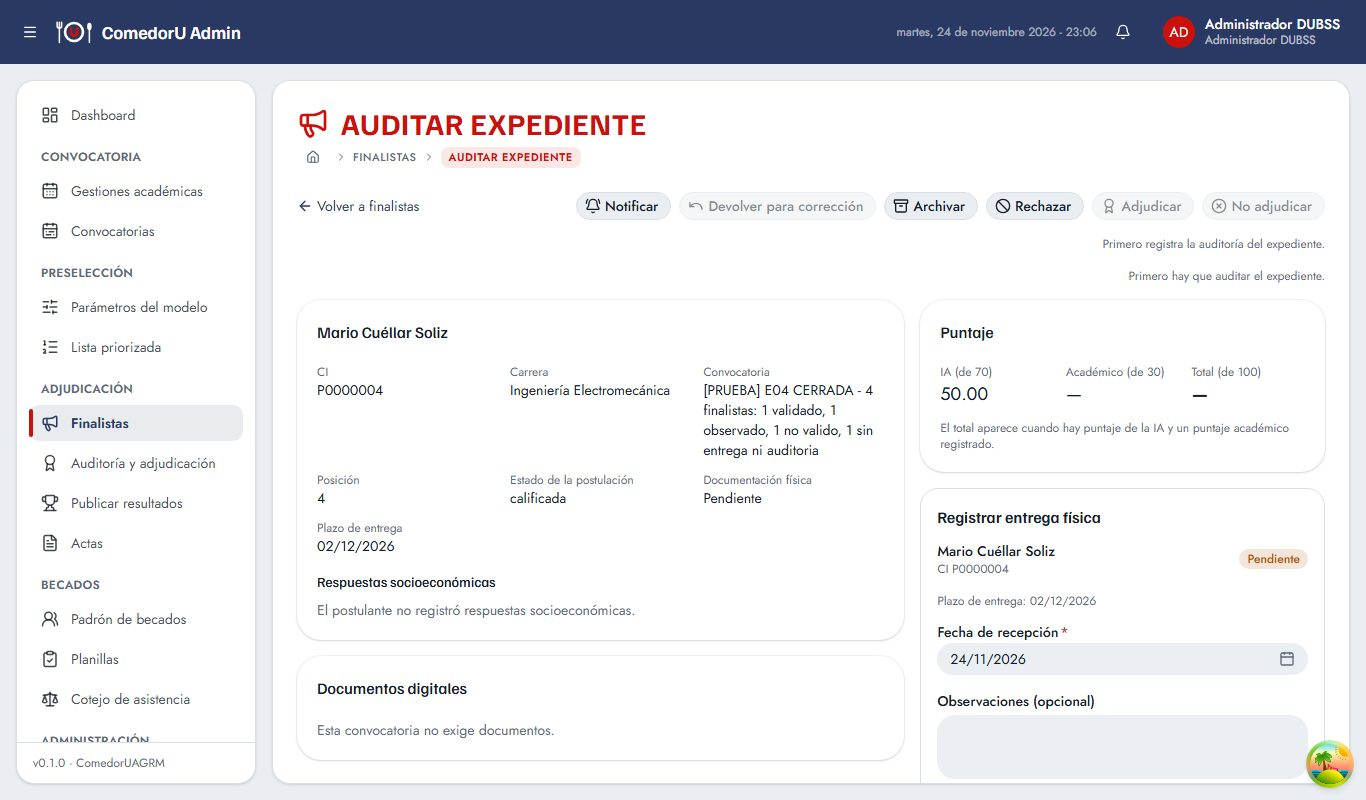
\includegraphics[width=0.93\linewidth,height=4.8cm,keepaspectratio]{images/168_CN_CU-05_B_final.jpg}}\vspace{2pt}\end{minipage}} \\
Resultado de prueba & {\textcolor{green!45!black}{\textbf{CORRECTO}}} \\
\end{longtable}
\endgroup
\addtocounter{table}{-1}
\vspace{-0.5\baselineskip}

\refstepcounter{table}\label{tab:cn_cu05_c}
\addcontentsline{lot}{table}{\protect\numberline{\thetable}CU-05. Auditar y adjudicar becas (motivo de no adjudicación)}
\noindent\textbf{Tabla~\thetable}\par\nopagebreak
\noindent\textit{CU-05. Auditar y adjudicar becas (motivo de no adjudicación)}\par\nopagebreak
\begingroup\footnotesize\linespread{1}\selectfont
\setlength{\LTleft}{0pt}\setlength{\LTright}{\fill}
\begin{longtable}{>{\raggedright\arraybackslash}p{3.6cm} >{\raggedright\arraybackslash}p{11.4cm}}
\toprule
\textbf{Campo} & \textbf{Contenido} \\
\midrule
\endfirsthead
\toprule
\textbf{Campo} & \textbf{Contenido} \\
\midrule
\endhead
\midrule
\multicolumn{2}{r}{\textit{Continúa en la siguiente página}} \\
\endfoot
\bottomrule
\multicolumn{2}{l}{\textit{Nota.} Elaboración propia a partir de la ejecución de la prueba.} \\
\endlastfoot
Nombre del caso de prueba & {CU-05. Auditar y adjudicar becas (motivo de no adjudicación)} \\
Descripción & {La no adjudicación exige un motivo.} \\
Precondición & {Finalista 2 (Ana Zambrana Heredia) de «[PRUEBA] E03», validado, puntaje total 83,00.} \\
Datos de entrada & {Motivo vacío.} \\
Condición de ejecución & {No aplica} \\
Captura de imagen inicial & {\begin{minipage}[t]{\linewidth}\strut\par\vspace{3pt}\fcolorbox{gray}{white}{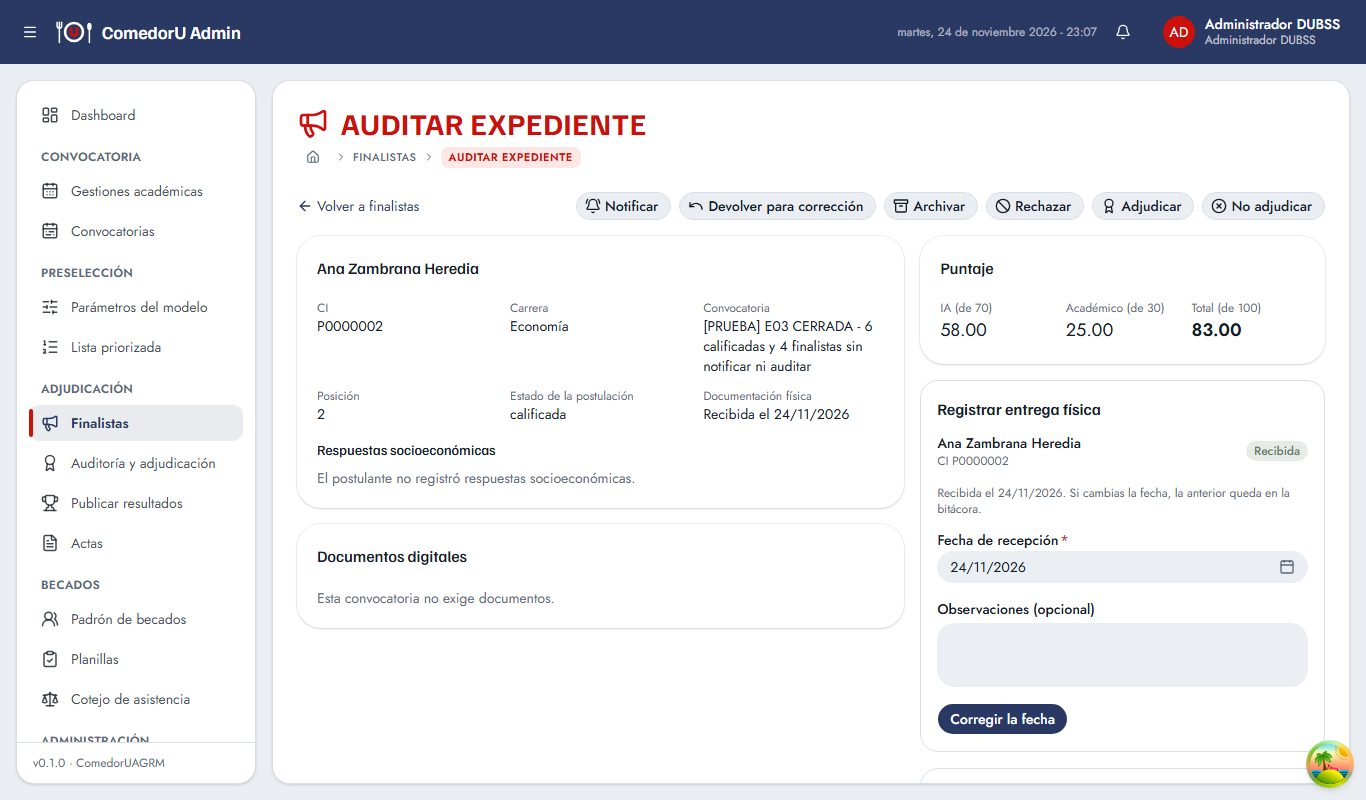
\includegraphics[width=0.93\linewidth,height=4.8cm,keepaspectratio]{images/169_CN_CU-05_C_inicial.jpg}}\vspace{2pt}\end{minipage}} \\
Pasos & {1. Abrir el expediente y pulsar «No adjudicar».\newline 2. Pulsar «No adjudicar» en la ventana sin escribir el motivo.} \\
Resultado esperado & {No se registra la decisión y se muestra que el motivo es obligatorio.} \\
Resultado obtenido & {La ventana siguió abierta con «El motivo es obligatorio» (puntaje total 83,00, cupos disponibles 3, mínimo 40,00).} \\
Captura de imagen final & {\begin{minipage}[t]{\linewidth}\strut\par\vspace{3pt}\fcolorbox{gray}{white}{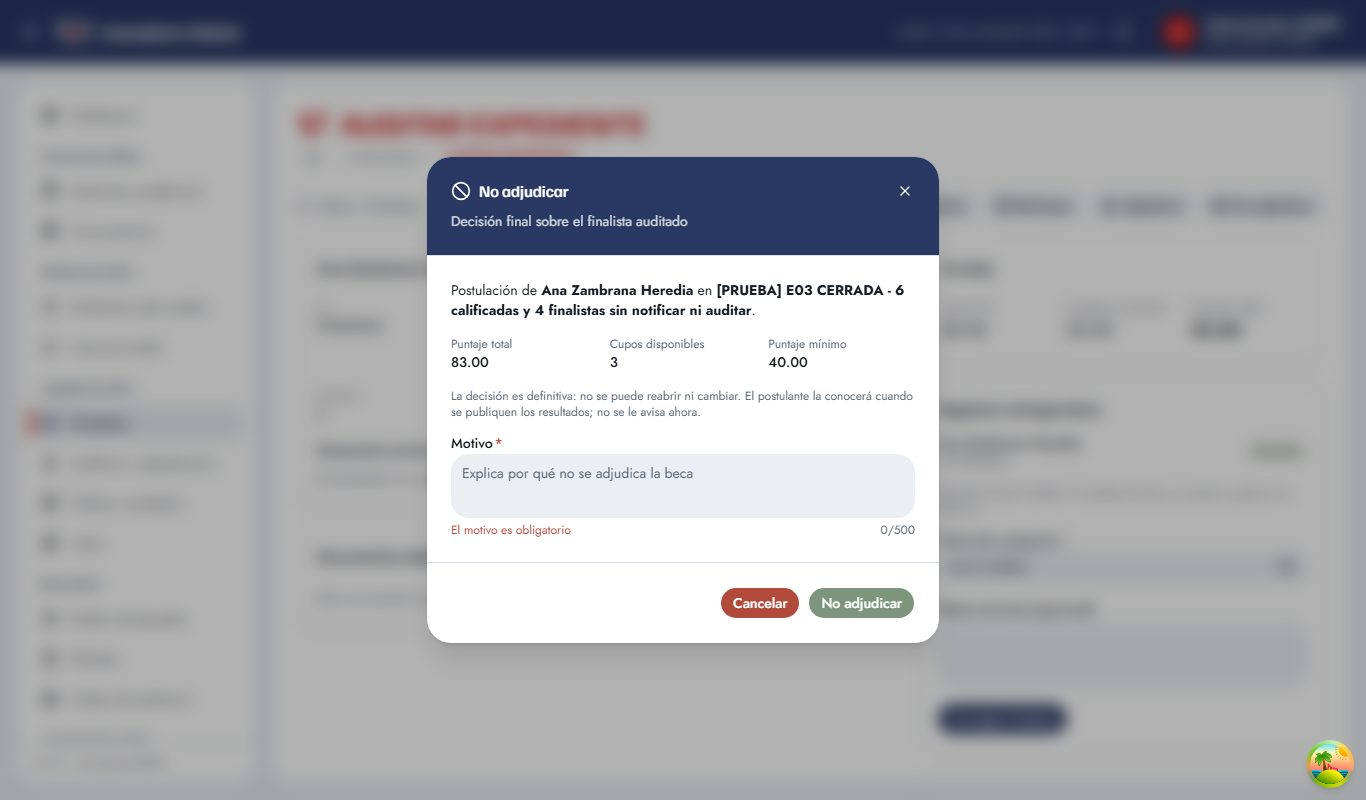
\includegraphics[width=0.93\linewidth,height=4.8cm,keepaspectratio]{images/170_CN_CU-05_C_final.jpg}}\vspace{2pt}\end{minipage}} \\
Resultado de prueba & {\textcolor{green!45!black}{\textbf{CORRECTO}}} \\
\end{longtable}
\endgroup
\addtocounter{table}{-1}
\vspace{-0.5\baselineskip}

\paragraph{CU-06. Visualizar lista priorizada de postulantes.}\label{sec:cn_cu06} 

\refstepcounter{table}\label{tab:cn_cu06_a}
\addcontentsline{lot}{table}{\protect\numberline{\thetable}CU-06. Visualizar lista priorizada de postulantes (consulta y exportación)}
\noindent\textbf{Tabla~\thetable}\par\nopagebreak
\noindent\textit{CU-06. Visualizar lista priorizada de postulantes (consulta y exportación)}\par\nopagebreak
\begingroup\footnotesize\linespread{1}\selectfont
\setlength{\LTleft}{0pt}\setlength{\LTright}{\fill}
\begin{longtable}{>{\raggedright\arraybackslash}p{3.6cm} >{\raggedright\arraybackslash}p{11.4cm}}
\toprule
\textbf{Campo} & \textbf{Contenido} \\
\midrule
\endfirsthead
\toprule
\textbf{Campo} & \textbf{Contenido} \\
\midrule
\endhead
\midrule
\multicolumn{2}{r}{\textit{Continúa en la siguiente página}} \\
\endfoot
\bottomrule
\multicolumn{2}{l}{\textit{Nota.} Elaboración propia a partir de la ejecución de la prueba.} \\
\endlastfoot
Nombre del caso de prueba & {CU-06. Visualizar lista priorizada de postulantes (consulta y exportación)} \\
Descripción & {El administrador consulta las postulaciones calificadas ordenadas por puntaje y exporta la lista completa.} \\
Precondición & {Sesión del Administrador DUBSS. Convocatoria sembrada «[PRUEBA] E02 CERRADA» con 6 postulaciones calificadas (puntajes de 65 a 35).} \\
Datos de entrada & {Convocatoria E02. Sin búsqueda ni filtro por carrera.} \\
Condición de ejecución & {No aplica} \\
Captura de imagen inicial & {\begin{minipage}[t]{\linewidth}\strut\par\vspace{3pt}\fcolorbox{gray}{white}{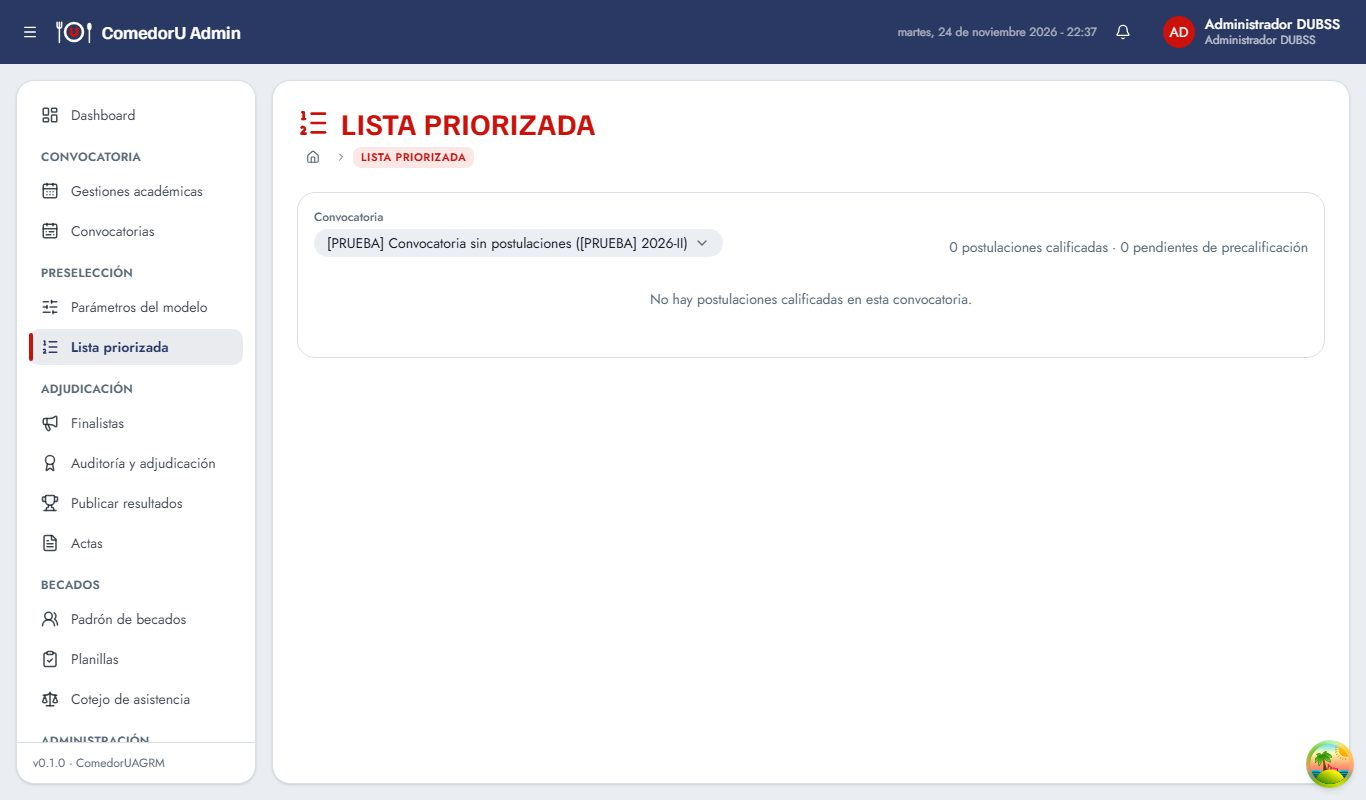
\includegraphics[width=0.93\linewidth,height=4.8cm,keepaspectratio]{images/171_CN_CU-06_A_inicial.jpg}}\vspace{2pt}\end{minipage}} \\
Pasos & {1. Abrir «Lista priorizada».\newline 2. Elegir la convocatoria E02.\newline 3. Revisar la tabla y pulsar «Exportar a PDF».} \\
Resultado esperado & {La tabla muestra posición, postulante, CI, carrera, puntaje y fecha de cálculo de mayor a menor puntaje, y se descarga un PDF con la lista.} \\
Resultado obtenido & {Se listaron 6 postulaciones en orden 65, 58, 52, 47, 41 y 35 con posiciones 1 a 6 («6 postulaciones calificadas · 0 pendientes de precalificación»). Se descargó \texttt{lista-\allowbreak{}priorizada-\allowbreak{}prueba-\allowbreak{}e02-\allowbreak{}.\allowbreak{}.\allowbreak{}.\allowbreak{}-\allowbreak{}20261124.\allowbreak{}pdf} (80 028 bytes) y apareció el aviso «Lista exportada».} \\
Captura de imagen final & {\begin{minipage}[t]{\linewidth}\strut\par\vspace{3pt}\fcolorbox{gray}{white}{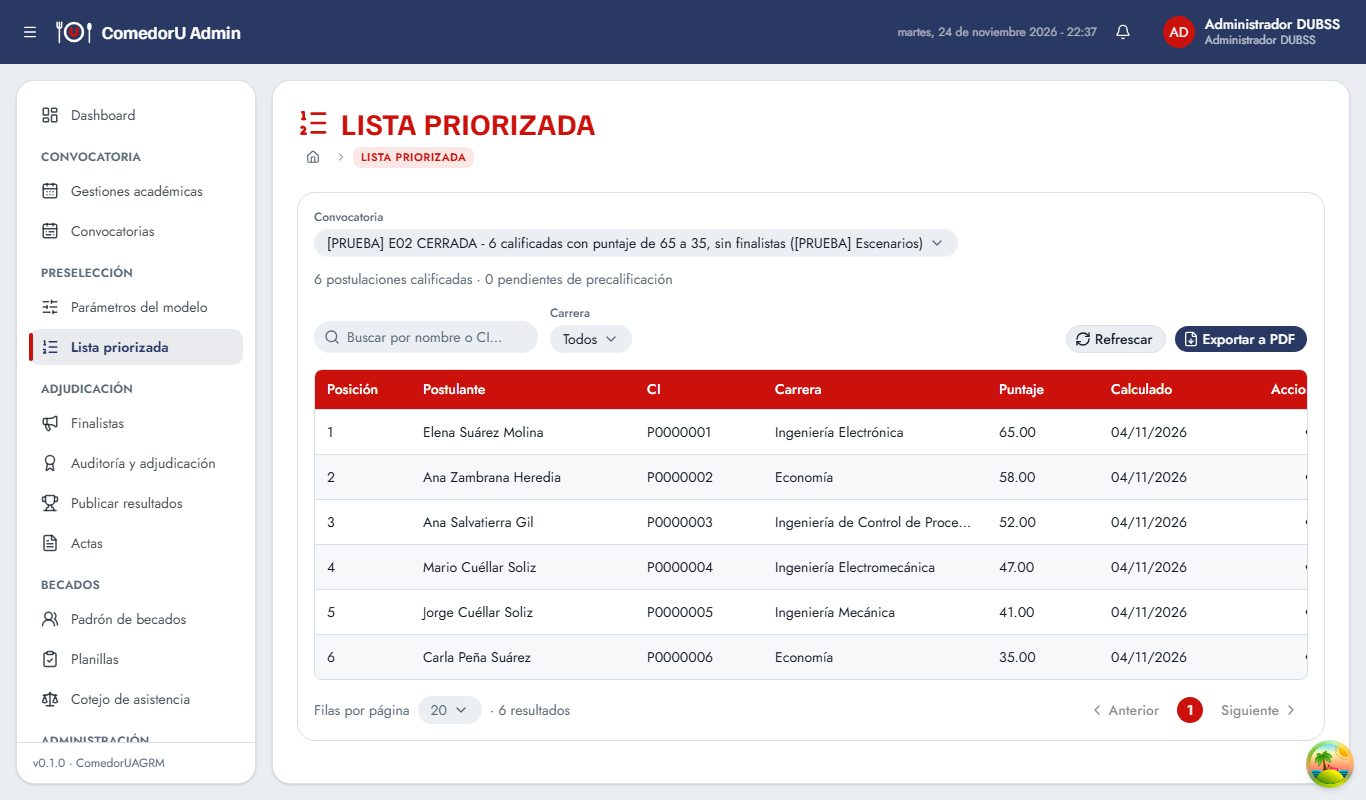
\includegraphics[width=0.93\linewidth,height=4.8cm,keepaspectratio]{images/172_CN_CU-06_A_lista_e02.jpg}}\vspace{2pt}\par\vspace{3pt}\fcolorbox{gray}{white}{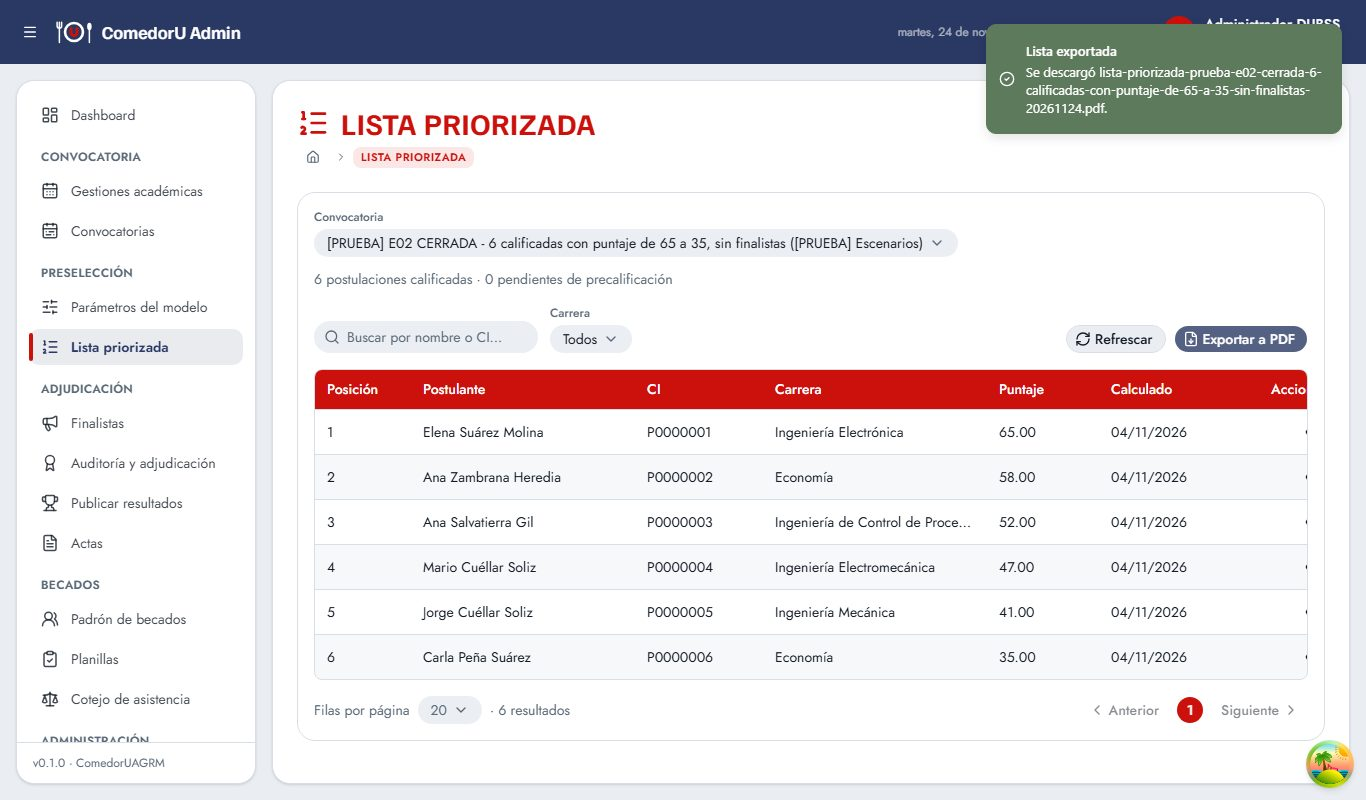
\includegraphics[width=0.93\linewidth,height=4.8cm,keepaspectratio]{images/173_CN_CU-06_A_final.jpg}}\vspace{2pt}\end{minipage}} \\
Resultado de prueba & {\textcolor{green!45!black}{\textbf{CORRECTO}}} \\
\end{longtable}
\endgroup
\addtocounter{table}{-1}
\vspace{-0.5\baselineskip}

\refstepcounter{table}\label{tab:cn_cu06_b}
\addcontentsline{lot}{table}{\protect\numberline{\thetable}CU-06. Visualizar lista priorizada de postulantes (lista vacía)}
\noindent\textbf{Tabla~\thetable}\par\nopagebreak
\noindent\textit{CU-06. Visualizar lista priorizada de postulantes (lista vacía)}\par\nopagebreak
\begingroup\footnotesize\linespread{1}\selectfont
\setlength{\LTleft}{0pt}\setlength{\LTright}{\fill}
\begin{longtable}{>{\raggedright\arraybackslash}p{3.6cm} >{\raggedright\arraybackslash}p{11.4cm}}
\toprule
\textbf{Campo} & \textbf{Contenido} \\
\midrule
\endfirsthead
\toprule
\textbf{Campo} & \textbf{Contenido} \\
\midrule
\endhead
\midrule
\multicolumn{2}{r}{\textit{Continúa en la siguiente página}} \\
\endfoot
\bottomrule
\multicolumn{2}{l}{\textit{Nota.} Elaboración propia a partir de la ejecución de la prueba.} \\
\endlastfoot
Nombre del caso de prueba & {CU-06. Visualizar lista priorizada de postulantes (lista vacía)} \\
Descripción & {El sistema informa cuando la convocatoria no tiene postulaciones calificadas.} \\
Precondición & {Sesión del administrador. Convocatoria «[PRUEBA] Convocatoria sin postulaciones».} \\
Datos de entrada & {Convocatoria «sin postulaciones».} \\
Condición de ejecución & {No aplica} \\
Captura de imagen inicial & {No aplica: la prueba comprueba un estado y no tiene pantalla previa distinta de la final.} \\
Pasos & {1. Abrir «Lista priorizada».\newline 2. Elegir la convocatoria sin postulaciones.} \\
Resultado esperado & {Se muestra un mensaje informativo y no se muestra la tabla.} \\
Resultado obtenido & {Se mostró «0 postulaciones calificadas · 0 pendientes de precalificación» y «No hay postulaciones calificadas en esta convocatoria.».} \\
Captura de imagen final & {\begin{minipage}[t]{\linewidth}\strut\par\vspace{3pt}\fcolorbox{gray}{white}{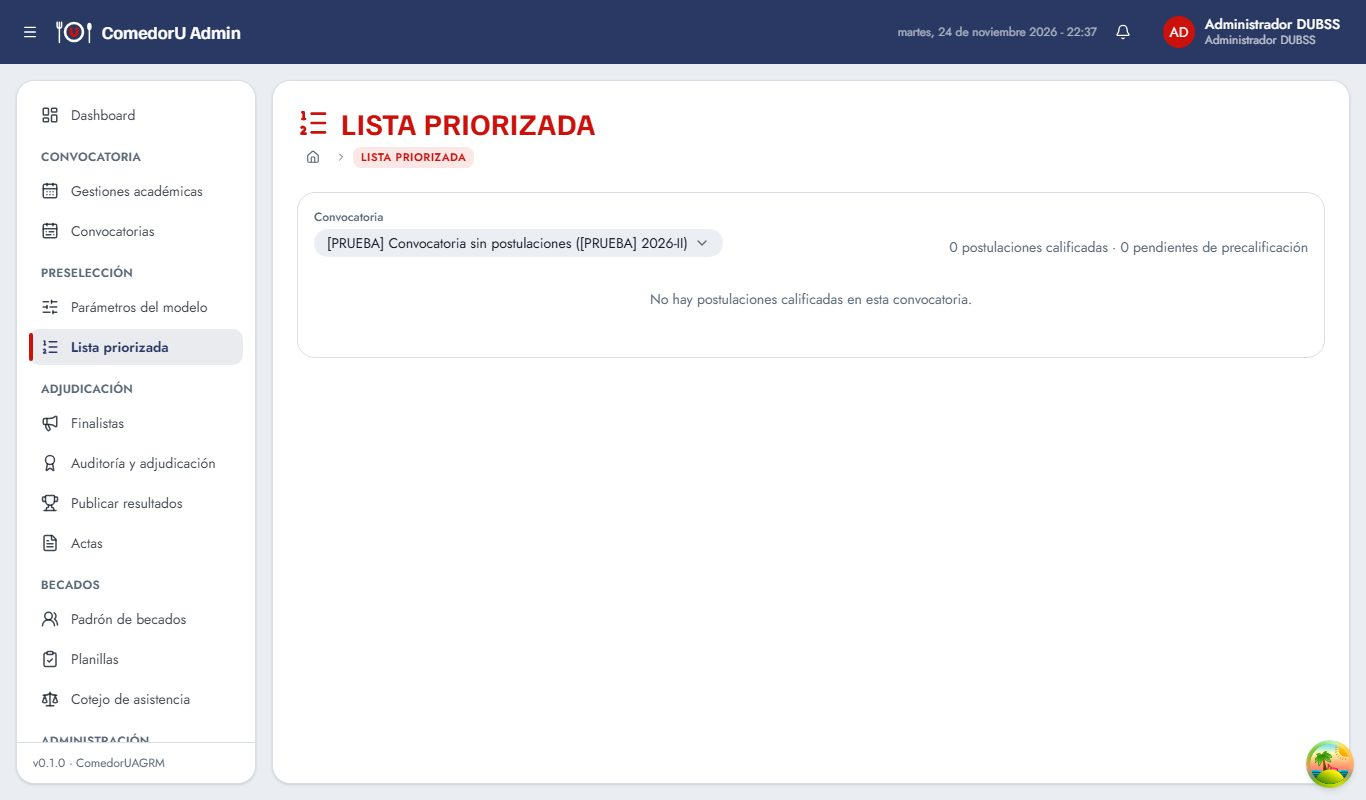
\includegraphics[width=0.93\linewidth,height=4.8cm,keepaspectratio]{images/174_CN_CU-06_B_final.jpg}}\vspace{2pt}\end{minipage}} \\
Resultado de prueba & {\textcolor{green!45!black}{\textbf{CORRECTO}}} \\
\end{longtable}
\endgroup
\addtocounter{table}{-1}
\vspace{-0.5\baselineskip}

\refstepcounter{table}\label{tab:cn_cu06_c}
\addcontentsline{lot}{table}{\protect\numberline{\thetable}CU-06. Visualizar lista priorizada de postulantes (control de acceso)}
\noindent\textbf{Tabla~\thetable}\par\nopagebreak
\noindent\textit{CU-06. Visualizar lista priorizada de postulantes (control de acceso)}\par\nopagebreak
\begingroup\footnotesize\linespread{1}\selectfont
\setlength{\LTleft}{0pt}\setlength{\LTright}{\fill}
\begin{longtable}{>{\raggedright\arraybackslash}p{3.6cm} >{\raggedright\arraybackslash}p{11.4cm}}
\toprule
\textbf{Campo} & \textbf{Contenido} \\
\midrule
\endfirsthead
\toprule
\textbf{Campo} & \textbf{Contenido} \\
\midrule
\endhead
\midrule
\multicolumn{2}{r}{\textit{Continúa en la siguiente página}} \\
\endfoot
\bottomrule
\multicolumn{2}{l}{\textit{Nota.} Elaboración propia a partir de la ejecución de la prueba.} \\
\endlastfoot
Nombre del caso de prueba & {CU-06. Visualizar lista priorizada de postulantes (control de acceso)} \\
Descripción & {Solo el administrador puede ver la lista.} \\
Precondición & {Sesión del postulante \texttt{postulante.\allowbreak{}finalista@\allowbreak{}prueba.\allowbreak{}local}.} \\
Datos de entrada & {Ruta \texttt{/\allowbreak{}lista-\allowbreak{}priorizada}.} \\
Condición de ejecución & {No aplica} \\
Captura de imagen inicial & {No aplica: la prueba comprueba un estado y no tiene pantalla previa distinta de la final.} \\
Pasos & {1. Iniciar sesión como postulante.\newline 2. Escribir en el navegador la ruta \texttt{/\allowbreak{}lista-\allowbreak{}priorizada}.} \\
Resultado esperado & {El sistema no muestra la pantalla y devuelve al postulante a su módulo.} \\
Resultado obtenido & {La aplicación redirigió a \texttt{/\allowbreak{}panel}.} \\
Captura de imagen final & {\begin{minipage}[t]{\linewidth}\strut\par\vspace{3pt}\fcolorbox{gray}{white}{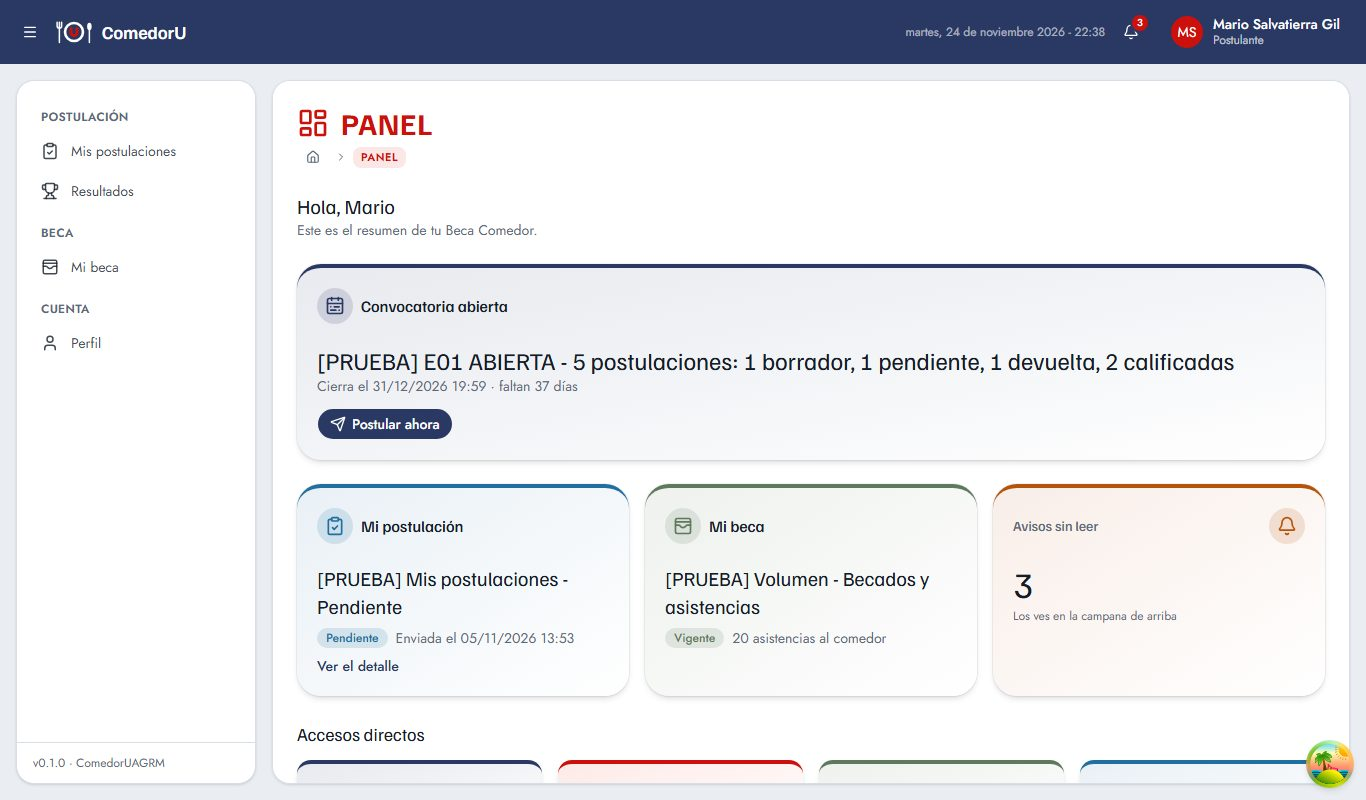
\includegraphics[width=0.93\linewidth,height=4.8cm,keepaspectratio]{images/175_CN_CU-06_C_final.jpg}}\vspace{2pt}\end{minipage}} \\
Resultado de prueba & {\textcolor{green!45!black}{\textbf{CORRECTO}}} \\
\end{longtable}
\endgroup
\addtocounter{table}{-1}
\vspace{-0.5\baselineskip}

\paragraph{CU-07. Auditar expediente finalista.}\label{sec:cn_cu07} 

\refstepcounter{table}\label{tab:cn_cu07_a}
\addcontentsline{lot}{table}{\protect\numberline{\thetable}CU-07. Auditar expediente finalista (validación)}
\noindent\textbf{Tabla~\thetable}\par\nopagebreak
\noindent\textit{CU-07. Auditar expediente finalista (validación)}\par\nopagebreak
\begingroup\footnotesize\linespread{1}\selectfont
\setlength{\LTleft}{0pt}\setlength{\LTright}{\fill}
\begin{longtable}{>{\raggedright\arraybackslash}p{3.6cm} >{\raggedright\arraybackslash}p{11.4cm}}
\toprule
\textbf{Campo} & \textbf{Contenido} \\
\midrule
\endfirsthead
\toprule
\textbf{Campo} & \textbf{Contenido} \\
\midrule
\endhead
\midrule
\multicolumn{2}{r}{\textit{Continúa en la siguiente página}} \\
\endfoot
\bottomrule
\multicolumn{2}{l}{\textit{Nota.} Elaboración propia a partir de la ejecución de la prueba.} \\
\endlastfoot
Nombre del caso de prueba & {CU-07. Auditar expediente finalista (validación)} \\
Descripción & {El administrador revisa el expediente de un finalista, registra la recepción de su documentación y lo audita con puntaje académico.} \\
Precondición & {Sesión del administrador. Finalista 2 (Ana Zambrana Heredia) de «[PRUEBA] E03», calificada, sin auditoría.} \\
Datos de entrada & {Fecha de recepción de hoy, resultado «Validado», puntaje académico 25.} \\
Condición de ejecución & {La documentación física debe estar registrada antes de auditar; el puntaje académico va de 0 a 30.} \\
Captura de imagen inicial & {\begin{minipage}[t]{\linewidth}\strut\par\vspace{3pt}\fcolorbox{gray}{white}{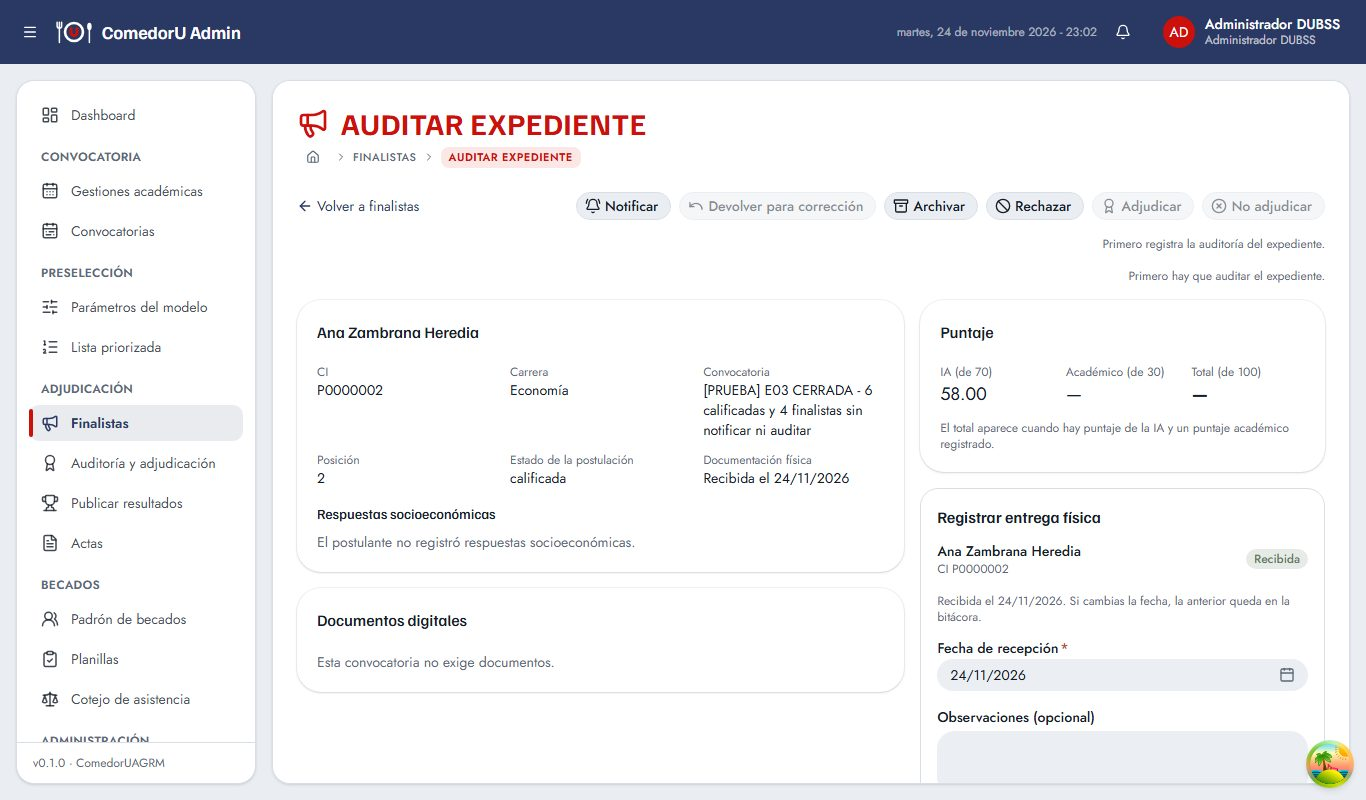
\includegraphics[width=0.93\linewidth,height=4.8cm,keepaspectratio]{images/176_CN_CU-07_A_inicial.jpg}}\vspace{2pt}\end{minipage}} \\
Pasos & {1. Abrir «Finalistas», elegir E03 y pulsar «Auditar» en Ana Zambrana.\newline 2. Registrar la entrega física («Marcar como recibida»).\newline 3. Elegir «Validado» y escribir 25 como puntaje académico.\newline 4. Pulsar «Registrar auditoría» y «Confirmar».} \\
Resultado esperado & {La auditoría queda en el historial y el total es el puntaje de la IA más el académico.} \\
Resultado obtenido & {Puntaje IA 58,00, académico 25,00 y total 83,00; el historial muestra «Validado … Administrador DUBSS · Académico 25.00». Nota: la entrega física ya estaba registrada cuando se tomó esta captura (un intento previo de la prueba la había registrado), por eso la captura inicial ya la muestra.} \\
Captura de imagen final & {\begin{minipage}[t]{\linewidth}\strut\par\vspace{3pt}\fcolorbox{gray}{white}{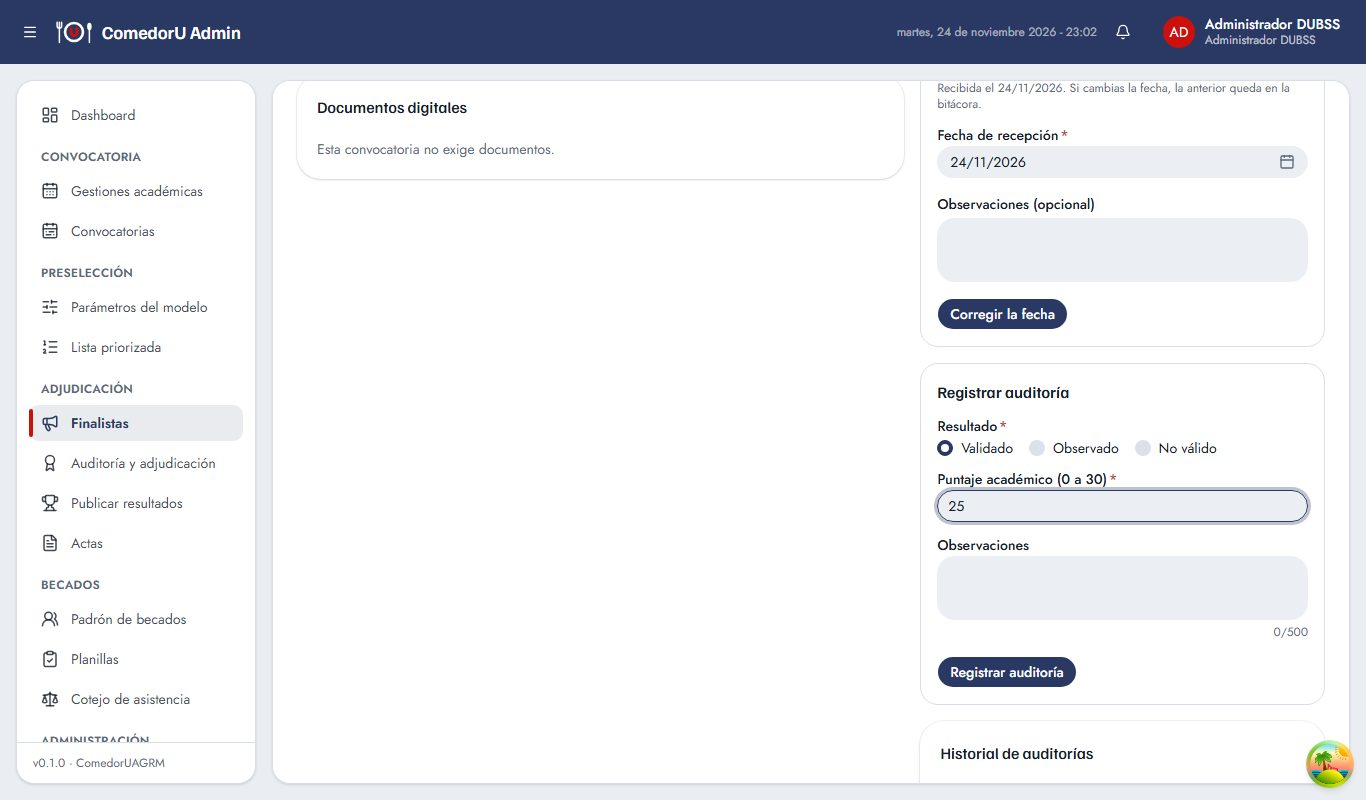
\includegraphics[width=0.93\linewidth,height=4.8cm,keepaspectratio]{images/177_CN_CU-07_A_formulario.jpg}}\vspace{2pt}\par\vspace{3pt}\fcolorbox{gray}{white}{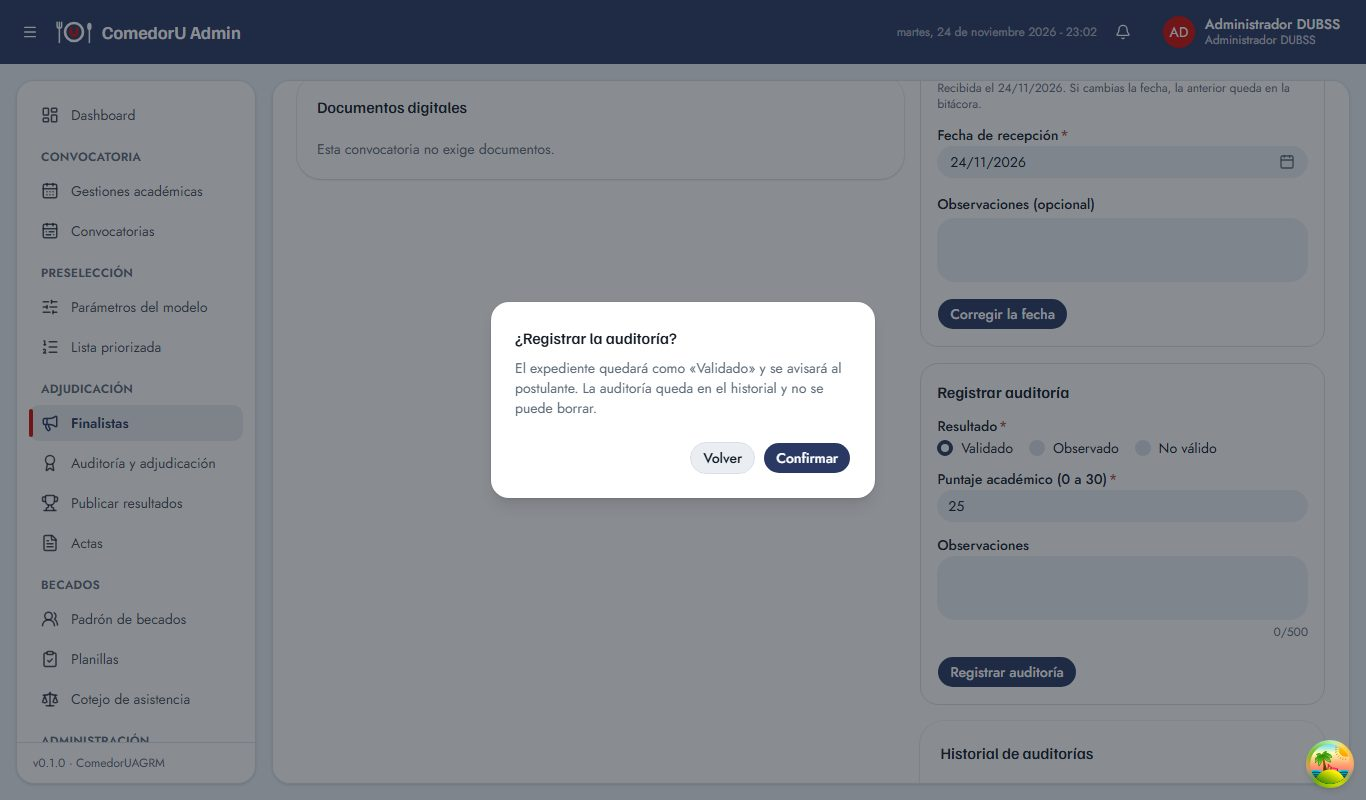
\includegraphics[width=0.93\linewidth,height=4.8cm,keepaspectratio]{images/178_CN_CU-07_A_confirmacion.jpg}}\vspace{2pt}\par\vspace{3pt}\fcolorbox{gray}{white}{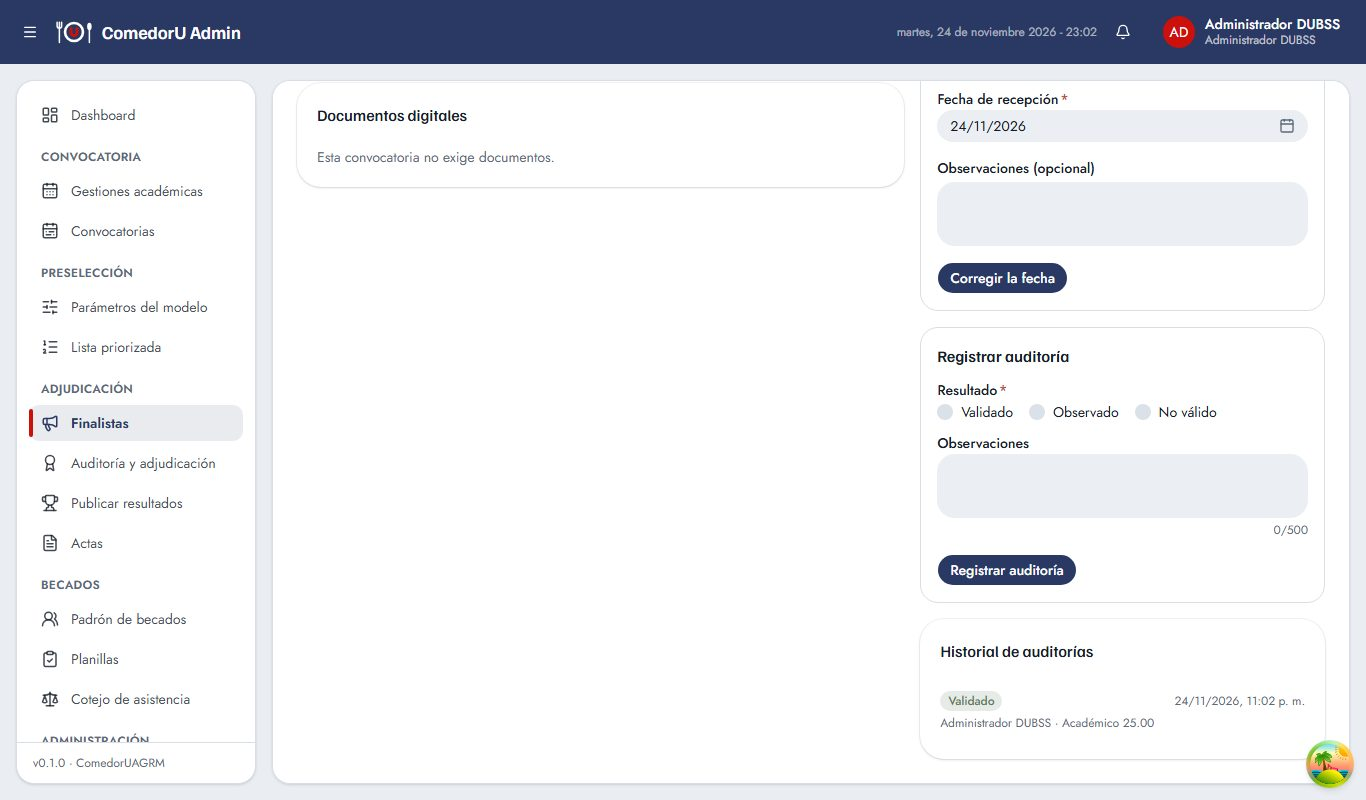
\includegraphics[width=0.93\linewidth,height=4.8cm,keepaspectratio]{images/179_CN_CU-07_A_final.jpg}}\vspace{2pt}\end{minipage}} \\
Resultado de prueba & {\textcolor{green!45!black}{\textbf{CORRECTO}}} \\
\end{longtable}
\endgroup
\addtocounter{table}{-1}
\vspace{-0.5\baselineskip}

\refstepcounter{table}\label{tab:cn_cu07_b}
\addcontentsline{lot}{table}{\protect\numberline{\thetable}CU-07. Auditar expediente finalista (observaciones obligatorias)}
\noindent\textbf{Tabla~\thetable}\par\nopagebreak
\noindent\textit{CU-07. Auditar expediente finalista (observaciones obligatorias)}\par\nopagebreak
\begingroup\footnotesize\linespread{1}\selectfont
\setlength{\LTleft}{0pt}\setlength{\LTright}{\fill}
\begin{longtable}{>{\raggedright\arraybackslash}p{3.6cm} >{\raggedright\arraybackslash}p{11.4cm}}
\toprule
\textbf{Campo} & \textbf{Contenido} \\
\midrule
\endfirsthead
\toprule
\textbf{Campo} & \textbf{Contenido} \\
\midrule
\endhead
\midrule
\multicolumn{2}{r}{\textit{Continúa en la siguiente página}} \\
\endfoot
\bottomrule
\multicolumn{2}{l}{\textit{Nota.} Elaboración propia a partir de la ejecución de la prueba.} \\
\endlastfoot
Nombre del caso de prueba & {CU-07. Auditar expediente finalista (observaciones obligatorias)} \\
Descripción & {Un expediente observado exige observaciones.} \\
Precondición & {Finalista 3 (Ana Salvatierra Gil) de E03 con entrega registrada.} \\
Datos de entrada & {Resultado «Observado» y el campo Observaciones vacío.} \\
Condición de ejecución & {No aplica} \\
Captura de imagen inicial & {\begin{minipage}[t]{\linewidth}\strut\par\vspace{3pt}\fcolorbox{gray}{white}{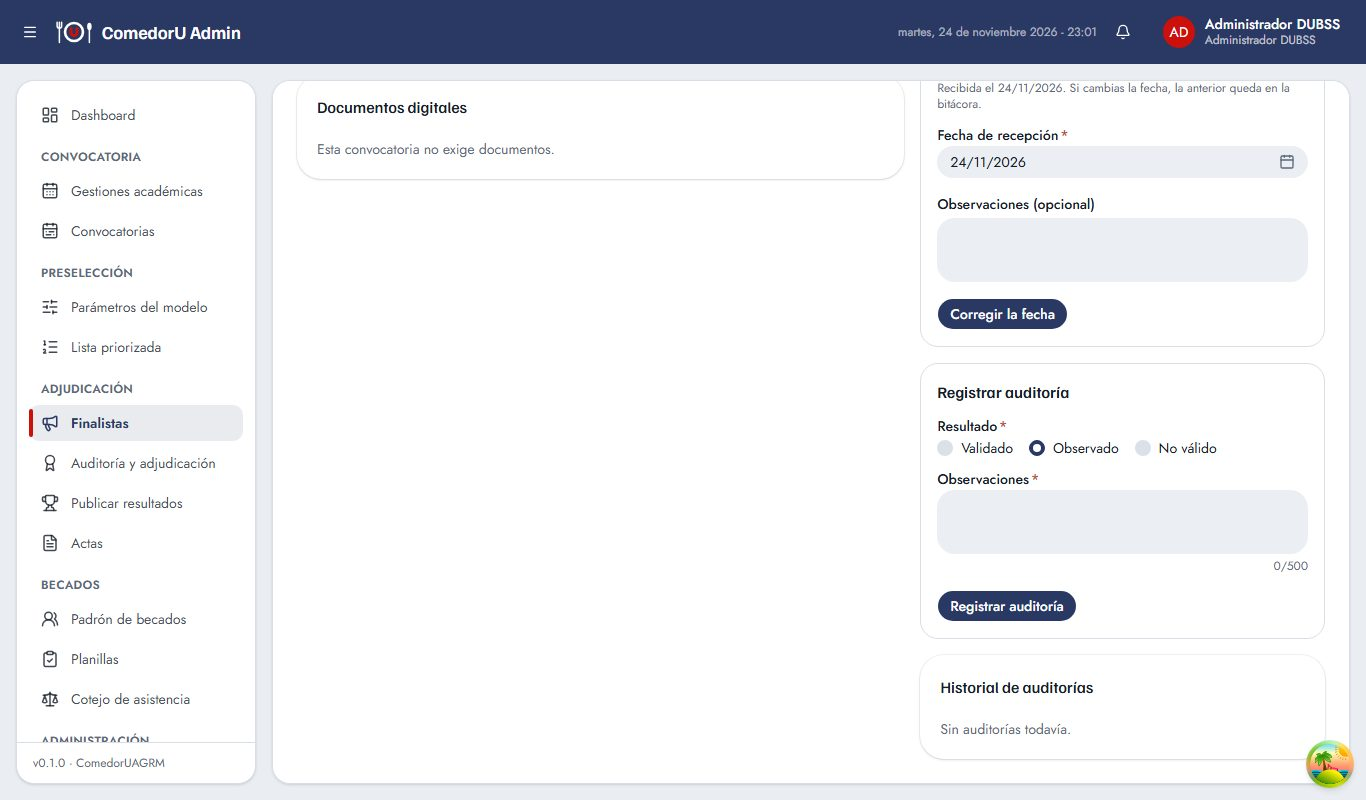
\includegraphics[width=0.93\linewidth,height=4.8cm,keepaspectratio]{images/180_CN_CU-07_B_inicial.jpg}}\vspace{2pt}\end{minipage}} \\
Pasos & {1. Abrir el expediente de Ana Salvatierra y registrar la entrega.\newline 2. Elegir «Observado» y dejar vacío «Observaciones».\newline 3. Pulsar «Registrar auditoría».} \\
Resultado esperado & {No se registra la auditoría y se indica que las observaciones son obligatorias.} \\
Resultado obtenido & {El formulario mostró «Las observaciones son obligatorias si el expediente es observado…» y el historial siguió con «Sin auditorías todavía».} \\
Captura de imagen final & {\begin{minipage}[t]{\linewidth}\strut\par\vspace{3pt}\fcolorbox{gray}{white}{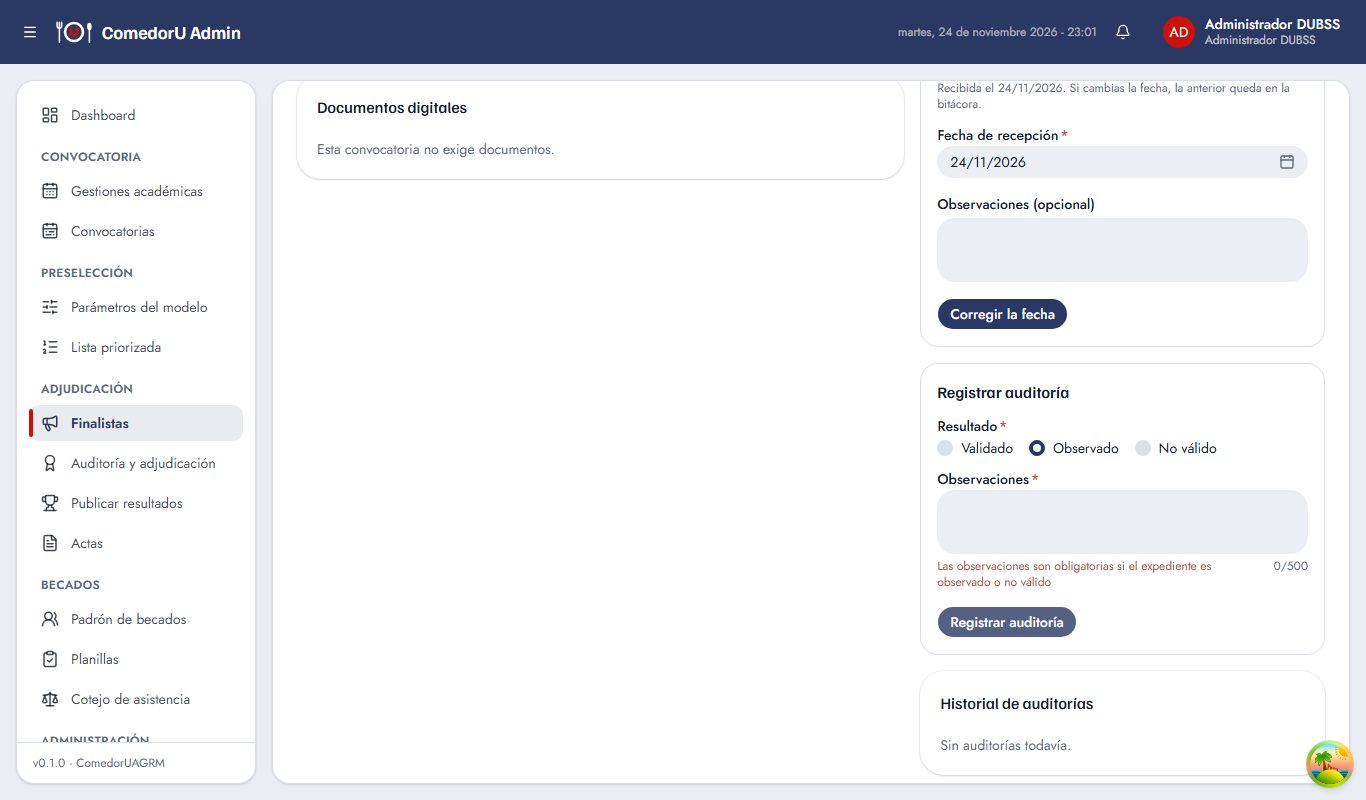
\includegraphics[width=0.93\linewidth,height=4.8cm,keepaspectratio]{images/181_CN_CU-07_B_final.jpg}}\vspace{2pt}\end{minipage}} \\
Resultado de prueba & {\textcolor{green!45!black}{\textbf{CORRECTO}}} \\
\end{longtable}
\endgroup
\addtocounter{table}{-1}
\vspace{-0.5\baselineskip}

\refstepcounter{table}\label{tab:cn_cu07_c}
\addcontentsline{lot}{table}{\protect\numberline{\thetable}CU-07. Auditar expediente finalista (entrega pendiente)}
\noindent\textbf{Tabla~\thetable}\par\nopagebreak
\noindent\textit{CU-07. Auditar expediente finalista (entrega pendiente)}\par\nopagebreak
\begingroup\footnotesize\linespread{1}\selectfont
\setlength{\LTleft}{0pt}\setlength{\LTright}{\fill}
\begin{longtable}{>{\raggedright\arraybackslash}p{3.6cm} >{\raggedright\arraybackslash}p{11.4cm}}
\toprule
\textbf{Campo} & \textbf{Contenido} \\
\midrule
\endfirsthead
\toprule
\textbf{Campo} & \textbf{Contenido} \\
\midrule
\endhead
\midrule
\multicolumn{2}{r}{\textit{Continúa en la siguiente página}} \\
\endfoot
\bottomrule
\multicolumn{2}{l}{\textit{Nota.} Elaboración propia a partir de la ejecución de la prueba.} \\
\endlastfoot
Nombre del caso de prueba & {CU-07. Auditar expediente finalista (entrega pendiente)} \\
Descripción & {No se puede auditar un expediente cuya documentación física no se recibió.} \\
Precondición & {Finalista 4 de «[PRUEBA] E04», sin entrega ni auditoría.} \\
Datos de entrada & {Expediente del finalista 4.} \\
Condición de ejecución & {No aplica} \\
Captura de imagen inicial & {No aplica: la prueba comprueba un estado y no tiene pantalla previa distinta de la final.} \\
Pasos & {1. Abrir «Finalistas», elegir E04 y «Auditar» en el finalista 4.\newline 2. Observar el formulario de auditoría.} \\
Resultado esperado & {El botón «Registrar auditoría» no está disponible y se pide registrar antes la entrega.} \\
Resultado obtenido & {Documentación física «Pendiente», aviso «Primero registra la entrega de la documentación física.» y botón «Registrar auditoría» deshabilitado.} \\
Captura de imagen final & {\begin{minipage}[t]{\linewidth}\strut\par\vspace{3pt}\fcolorbox{gray}{white}{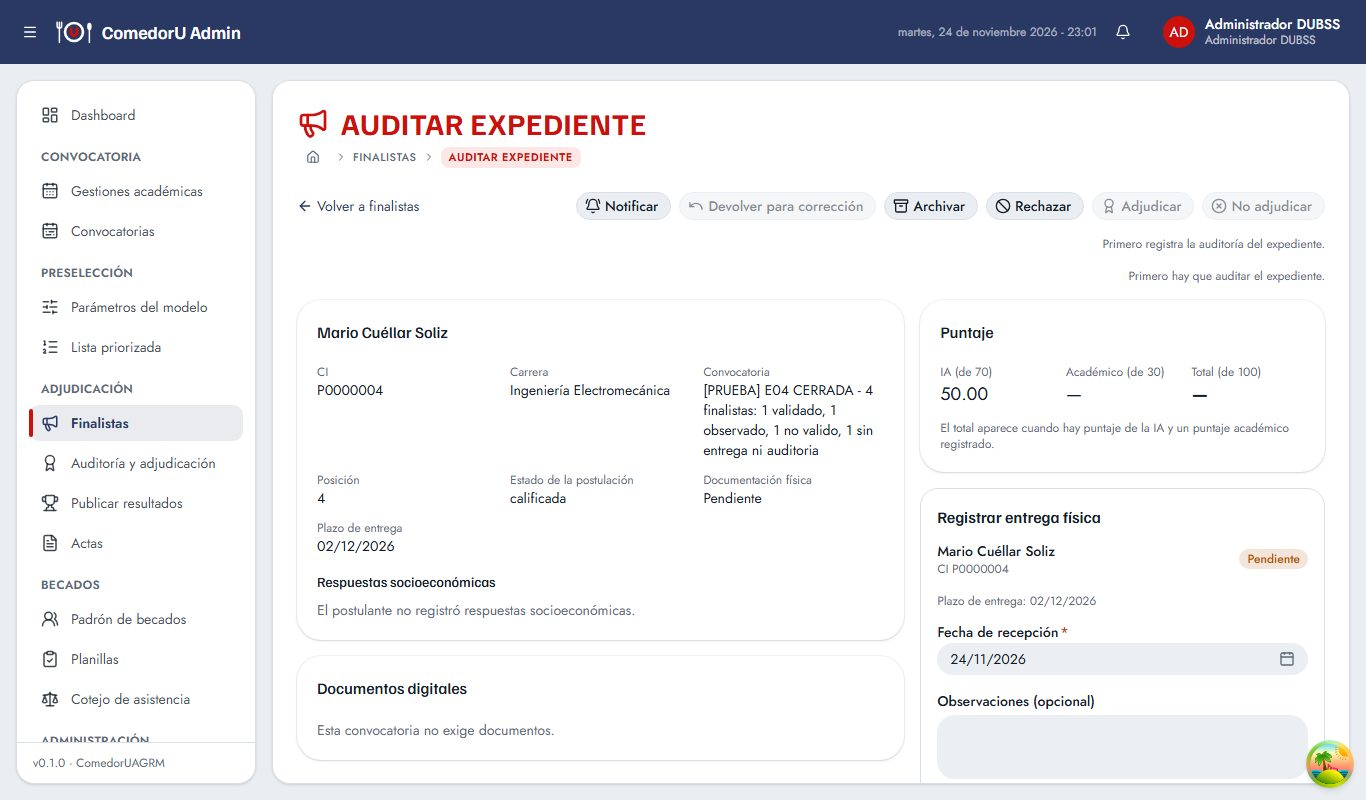
\includegraphics[width=0.93\linewidth,height=4.8cm,keepaspectratio]{images/182_CN_CU-07_C_final.jpg}}\vspace{2pt}\end{minipage}} \\
Resultado de prueba & {\textcolor{green!45!black}{\textbf{CORRECTO}}} \\
\end{longtable}
\endgroup
\addtocounter{table}{-1}
\vspace{-0.5\baselineskip}

\paragraph{CU-08. Generar acta de adjudicación.}\label{sec:cn_cu08} 

\refstepcounter{table}\label{tab:cn_cu08_a}
\addcontentsline{lot}{table}{\protect\numberline{\thetable}CU-08. Generar acta de adjudicación (generación)}
\noindent\textbf{Tabla~\thetable}\par\nopagebreak
\noindent\textit{CU-08. Generar acta de adjudicación (generación)}\par\nopagebreak
\begingroup\footnotesize\linespread{1}\selectfont
\setlength{\LTleft}{0pt}\setlength{\LTright}{\fill}
\begin{longtable}{>{\raggedright\arraybackslash}p{3.6cm} >{\raggedright\arraybackslash}p{11.4cm}}
\toprule
\textbf{Campo} & \textbf{Contenido} \\
\midrule
\endfirsthead
\toprule
\textbf{Campo} & \textbf{Contenido} \\
\midrule
\endhead
\midrule
\multicolumn{2}{r}{\textit{Continúa en la siguiente página}} \\
\endfoot
\bottomrule
\multicolumn{2}{l}{\textit{Nota.} Elaboración propia a partir de la ejecución de la prueba.} \\
\endlastfoot
Nombre del caso de prueba & {CU-08. Generar acta de adjudicación (generación)} \\
Descripción & {El administrador genera el acta definitiva en PDF con número automático para una convocatoria con resultados publicados.} \\
Precondición & {Convocatoria sembrada «[PRUEBA] E06», publicada y sin acta (3 adjudicados). MinIO activo.} \\
Datos de entrada & {Convocatoria E06.} \\
Condición de ejecución & {El acta es definitiva: no se puede regenerar ni eliminar.} \\
Captura de imagen inicial & {\begin{minipage}[t]{\linewidth}\strut\par\vspace{3pt}\fcolorbox{gray}{white}{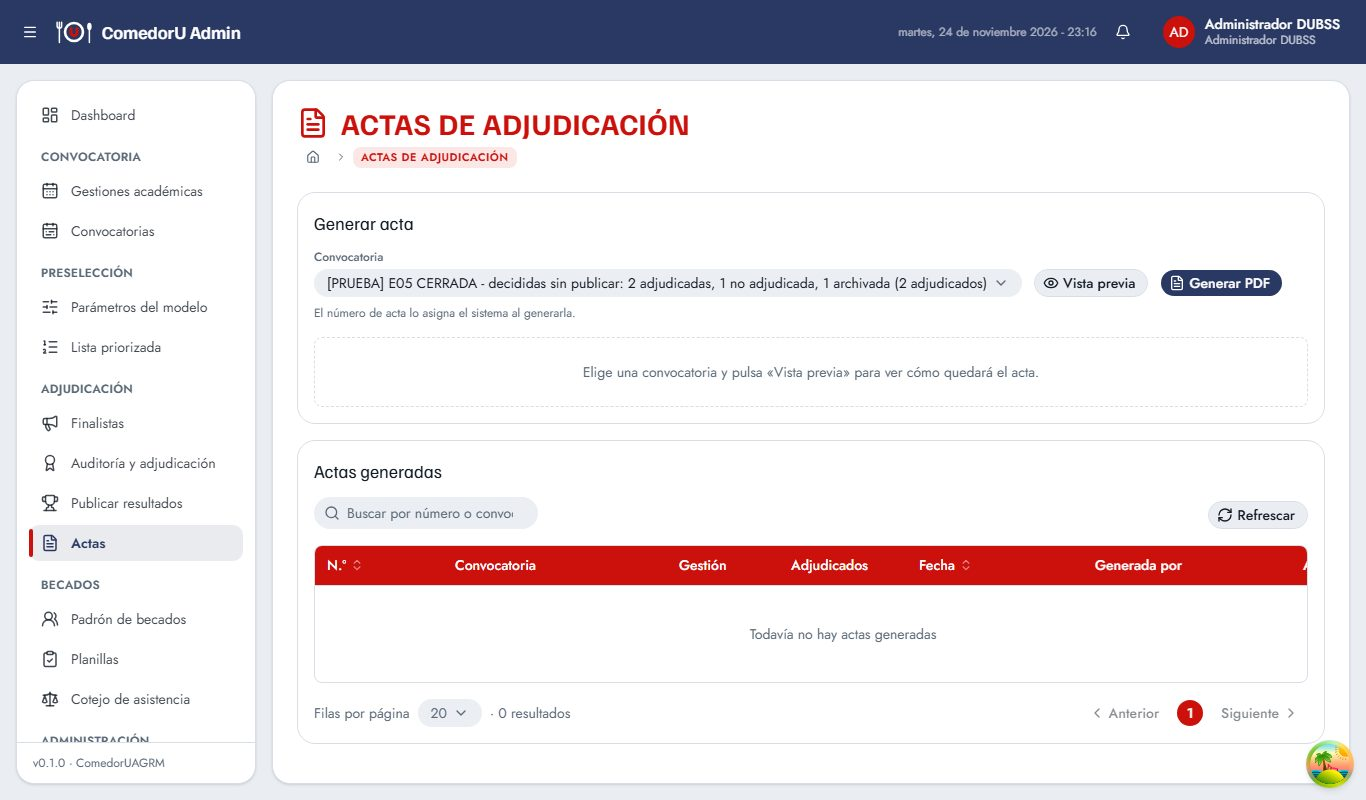
\includegraphics[width=0.93\linewidth,height=4.8cm,keepaspectratio]{images/183_CN_CU-08_A_inicial.jpg}}\vspace{2pt}\end{minipage}} \\
Pasos & {1. Abrir «Actas» y elegir E06.\newline 2. Pulsar «Vista previa».\newline 3. Pulsar «Generar PDF» y confirmar con «Generar».} \\
Resultado esperado & {Se genera el acta con número \texttt{NNN/\allowbreak{}AAAA} y aparece en la tabla de actas generadas.} \\
Resultado obtenido & {La tabla muestra el acta \texttt{001/\allowbreak{}2026}, 3 adjudicados, generada por Administrador DUBSS el 24/11/2026.} \\
Captura de imagen final & {\begin{minipage}[t]{\linewidth}\strut\par\vspace{3pt}\fcolorbox{gray}{white}{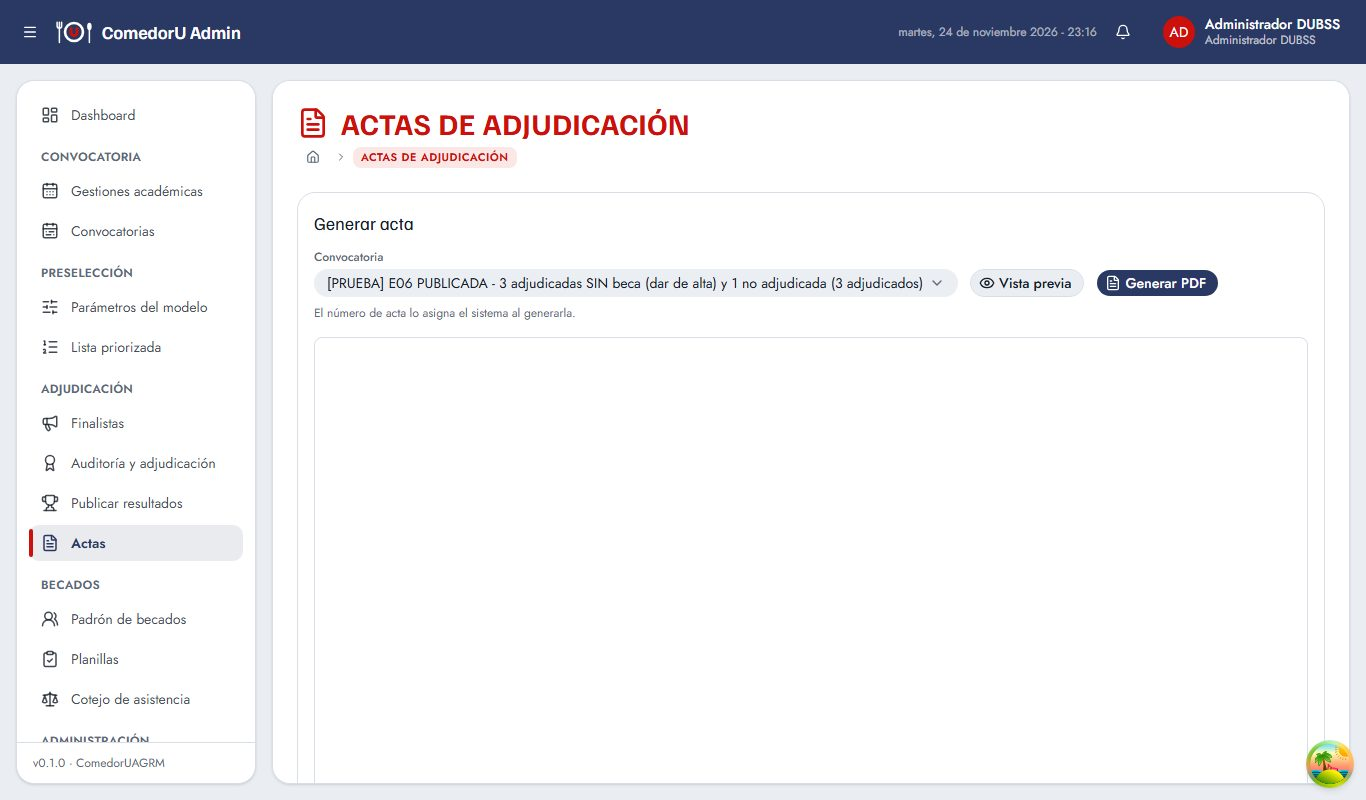
\includegraphics[width=0.93\linewidth,height=4.8cm,keepaspectratio]{images/184_CN_CU-08_A_vista_previa.jpg}}\vspace{2pt}\par\vspace{3pt}\fcolorbox{gray}{white}{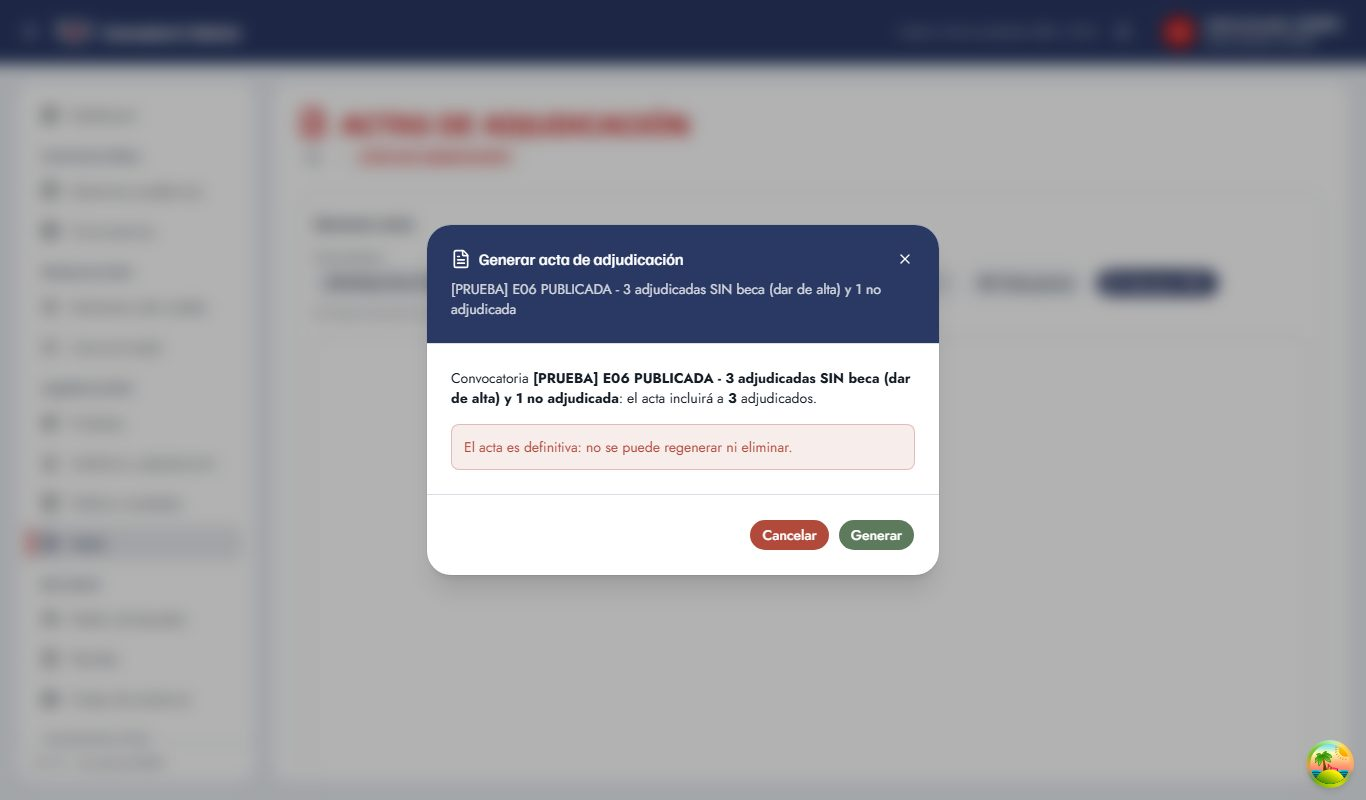
\includegraphics[width=0.93\linewidth,height=4.8cm,keepaspectratio]{images/185_CN_CU-08_A_confirmacion.jpg}}\vspace{2pt}\par\vspace{3pt}\fcolorbox{gray}{white}{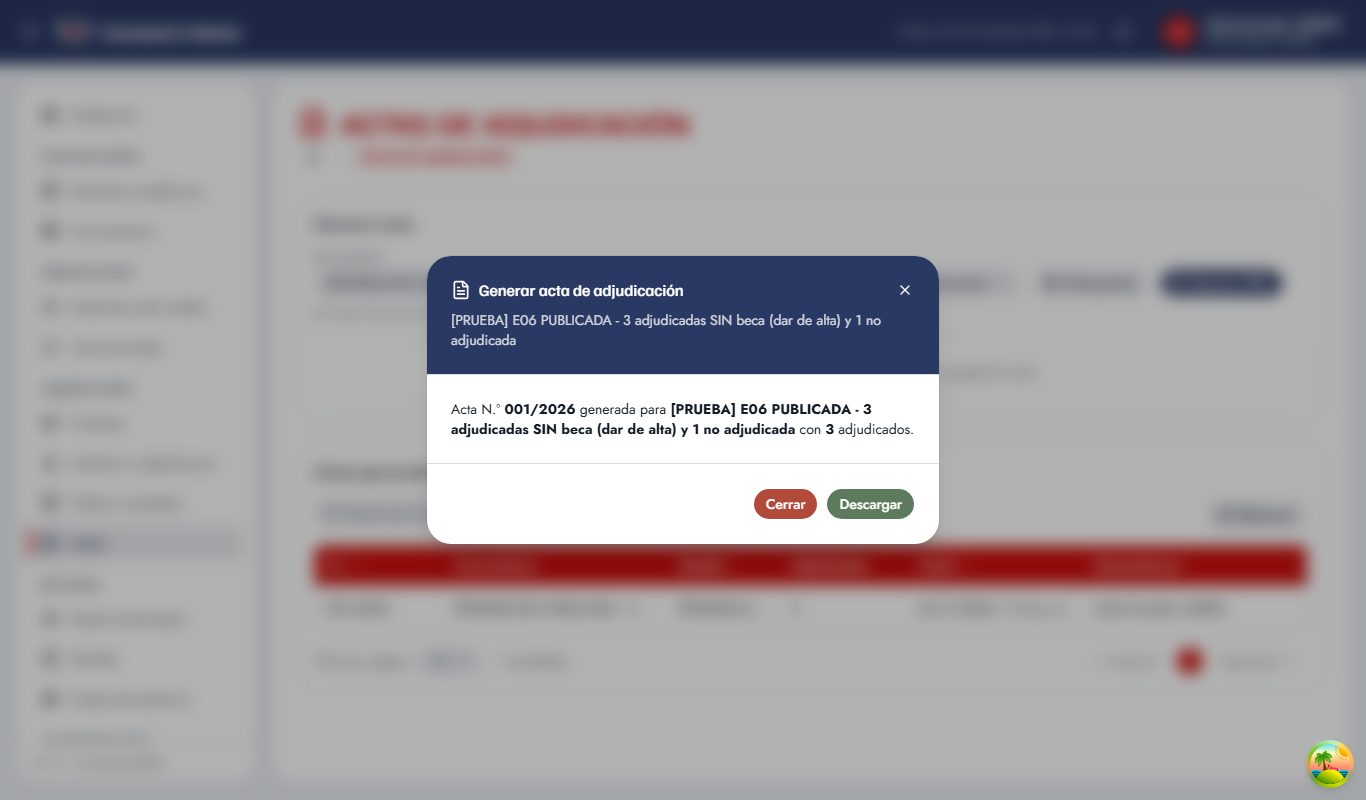
\includegraphics[width=0.93\linewidth,height=4.8cm,keepaspectratio]{images/186_CN_CU-08_A_final.jpg}}\vspace{2pt}\end{minipage}} \\
Resultado de prueba & {\textcolor{green!45!black}{\textbf{CORRECTO}}} \\
\end{longtable}
\endgroup
\addtocounter{table}{-1}
\vspace{-0.5\baselineskip}

\refstepcounter{table}\label{tab:cn_cu08_b}
\addcontentsline{lot}{table}{\protect\numberline{\thetable}CU-08. Generar acta de adjudicación (descarga)}
\noindent\textbf{Tabla~\thetable}\par\nopagebreak
\noindent\textit{CU-08. Generar acta de adjudicación (descarga)}\par\nopagebreak
\begingroup\footnotesize\linespread{1}\selectfont
\setlength{\LTleft}{0pt}\setlength{\LTright}{\fill}
\begin{longtable}{>{\raggedright\arraybackslash}p{3.6cm} >{\raggedright\arraybackslash}p{11.4cm}}
\toprule
\textbf{Campo} & \textbf{Contenido} \\
\midrule
\endfirsthead
\toprule
\textbf{Campo} & \textbf{Contenido} \\
\midrule
\endhead
\midrule
\multicolumn{2}{r}{\textit{Continúa en la siguiente página}} \\
\endfoot
\bottomrule
\multicolumn{2}{l}{\textit{Nota.} Elaboración propia a partir de la ejecución de la prueba.} \\
\endlastfoot
Nombre del caso de prueba & {CU-08. Generar acta de adjudicación (descarga)} \\
Descripción & {El administrador descarga el PDF del acta generada.} \\
Precondición & {Acta 001/2026 generada.} \\
Datos de entrada & {Acción «Descargar» de la fila del acta.} \\
Condición de ejecución & {No aplica} \\
Captura de imagen inicial & {No aplica: la prueba comprueba un estado y no tiene pantalla previa distinta de la final.} \\
Pasos & {1. En «Actas», pulsar «Descargar» en la fila del acta 001/2026.} \\
Resultado esperado & {Se descarga un PDF con el acta y los adjudicados.} \\
Resultado obtenido & {Se descargó \texttt{acta-\allowbreak{}001-\allowbreak{}2026.\allowbreak{}pdf} (79 735 bytes). Contiene «Acta de adjudicación», N.º 001/2026, cupos 3, puntaje mínimo 40,00 y a los 3 adjudicados con CI, carrera y puntaje final 95,00. El nombre largo de la convocatoria de prueba aparece cortado en el encabezado.} \\
Captura de imagen final & {\begin{minipage}[t]{\linewidth}\strut\par\vspace{3pt}\fcolorbox{gray}{white}{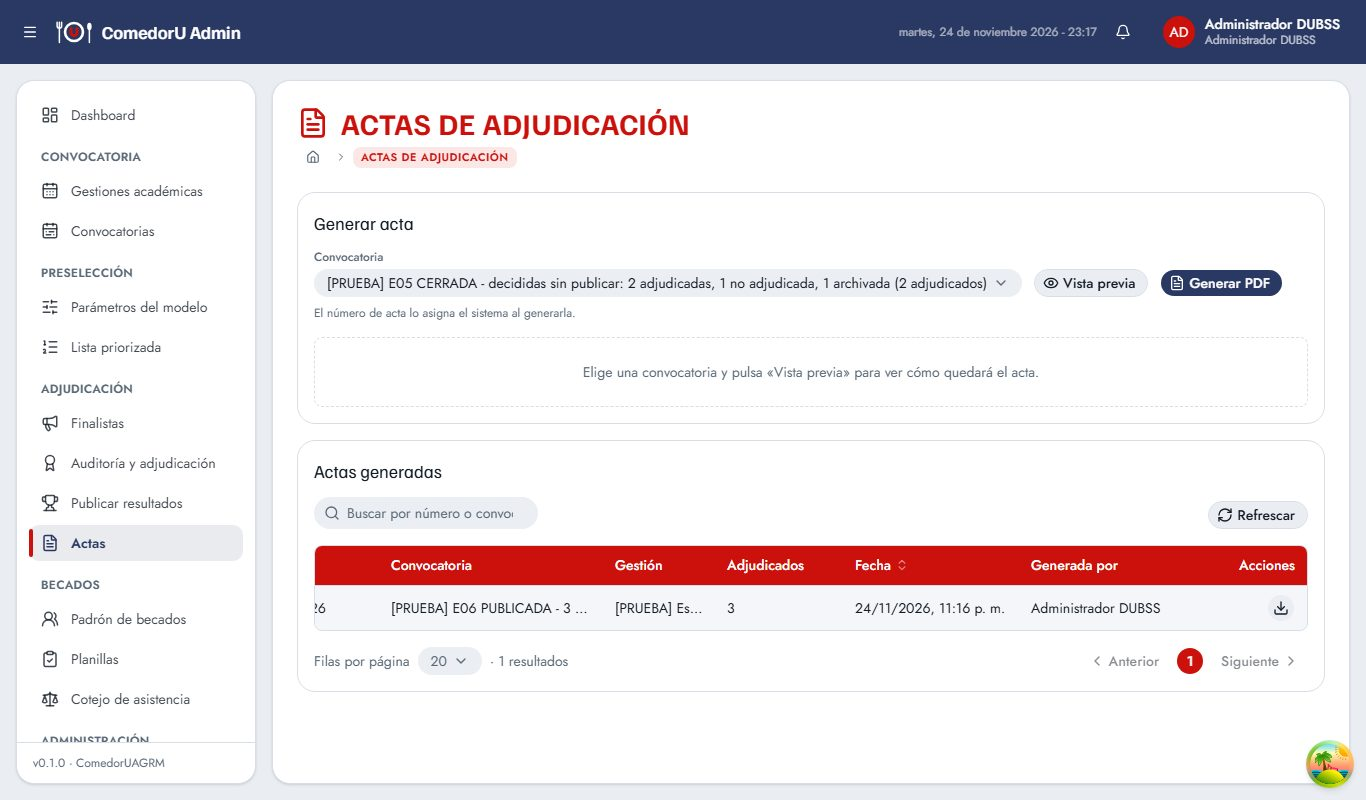
\includegraphics[width=0.93\linewidth,height=4.8cm,keepaspectratio]{images/187_CN_CU-08_B_final.jpg}}\vspace{2pt}\end{minipage}} \\
Resultado de prueba & {\textcolor{green!45!black}{\textbf{CORRECTO}}} \\
\end{longtable}
\endgroup
\addtocounter{table}{-1}
\vspace{-0.5\baselineskip}

\refstepcounter{table}\label{tab:cn_cu08_c}
\addcontentsline{lot}{table}{\protect\numberline{\thetable}CU-08. Generar acta de adjudicación (convocatoria sin resultados publicados)}
\noindent\textbf{Tabla~\thetable}\par\nopagebreak
\noindent\textit{CU-08. Generar acta de adjudicación (convocatoria sin resultados publicados)}\par\nopagebreak
\begingroup\footnotesize\linespread{1}\selectfont
\setlength{\LTleft}{0pt}\setlength{\LTright}{\fill}
\begin{longtable}{>{\raggedright\arraybackslash}p{3.6cm} >{\raggedright\arraybackslash}p{11.4cm}}
\toprule
\textbf{Campo} & \textbf{Contenido} \\
\midrule
\endfirsthead
\toprule
\textbf{Campo} & \textbf{Contenido} \\
\midrule
\endhead
\midrule
\multicolumn{2}{r}{\textit{Continúa en la siguiente página}} \\
\endfoot
\bottomrule
\multicolumn{2}{l}{\textit{Nota.} Elaboración propia a partir de la ejecución de la prueba.} \\
\endlastfoot
Nombre del caso de prueba & {CU-08. Generar acta de adjudicación (convocatoria sin resultados publicados)} \\
Descripción & {El selector solo ofrece convocatorias con resultados publicados que aún no tienen acta.} \\
Precondición & {Acta de E06 ya generada.} \\
Datos de entrada & {Selector de convocatoria.} \\
Condición de ejecución & {No aplica} \\
Captura de imagen inicial & {No aplica: la prueba comprueba un estado y no tiene pantalla previa distinta de la final.} \\
Pasos & {1. En «Actas», abrir la lista del selector «Convocatoria».} \\
Resultado esperado & {E06 (ya con acta) y las convocatorias sin resultados publicados no aparecen.} \\
Resultado obtenido & {El selector ofreció E05, E07, E08 y las convocatorias publicadas sin acta; E06 ya no aparecía.} \\
Captura de imagen final & {\begin{minipage}[t]{\linewidth}\strut\par\vspace{3pt}\fcolorbox{gray}{white}{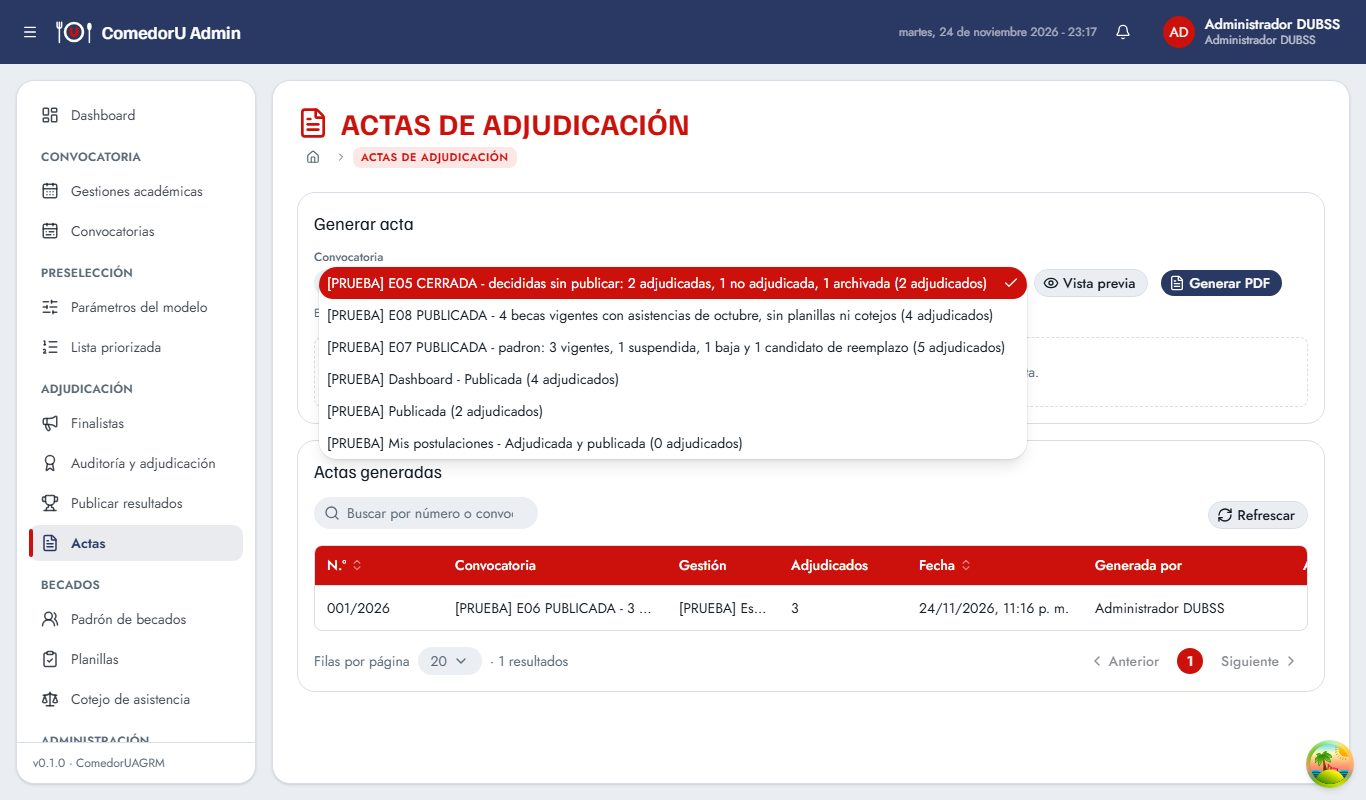
\includegraphics[width=0.93\linewidth,height=4.8cm,keepaspectratio]{images/188_CN_CU-08_C_final.jpg}}\vspace{2pt}\end{minipage}} \\
Resultado de prueba & {\textcolor{green!45!black}{\textbf{CORRECTO}}} \\
\end{longtable}
\endgroup
\addtocounter{table}{-1}
\vspace{-0.5\baselineskip}

\paragraph{CU-12. Visualizar dashboard de indicadores BI.}\label{sec:cn_cu12} 

\refstepcounter{table}\label{tab:cn_cu12_a}
\addcontentsline{lot}{table}{\protect\numberline{\thetable}CU-12. Visualizar dashboard de indicadores BI (selección sin datos)}
\noindent\textbf{Tabla~\thetable}\par\nopagebreak
\noindent\textit{CU-12. Visualizar dashboard de indicadores BI (selección sin datos)}\par\nopagebreak
\begingroup\footnotesize\linespread{1}\selectfont
\setlength{\LTleft}{0pt}\setlength{\LTright}{\fill}
\begin{longtable}{>{\raggedright\arraybackslash}p{3.6cm} >{\raggedright\arraybackslash}p{11.4cm}}
\toprule
\textbf{Campo} & \textbf{Contenido} \\
\midrule
\endfirsthead
\toprule
\textbf{Campo} & \textbf{Contenido} \\
\midrule
\endhead
\midrule
\multicolumn{2}{r}{\textit{Continúa en la siguiente página}} \\
\endfoot
\bottomrule
\multicolumn{2}{l}{\textit{Nota.} Elaboración propia a partir de la ejecución de la prueba.} \\
\endlastfoot
Nombre del caso de prueba & {CU-12. Visualizar dashboard de indicadores BI (selección sin datos)} \\
Descripción & {Al abrir el dashboard sin datos para la selección, el sistema lo informa y muestra los indicadores en cero.} \\
Precondición & {Sesión de \texttt{directivo@\allowbreak{}dubss.\allowbreak{}com}.} \\
Datos de entrada & {Selección por defecto (gestión «[PRUEBA] Escenarios»).} \\
Condición de ejecución & {No aplica} \\
Captura de imagen inicial & {No aplica: la prueba comprueba un estado y no tiene pantalla previa distinta de la final.} \\
Pasos & {1. Iniciar sesión como directivo.\newline 2. Observar el dashboard.} \\
Resultado esperado & {Mensaje informativo e indicadores en cero (no es un error).} \\
Resultado obtenido & {Se mostró «No hay datos para la selección elegida todavía.» con todos los indicadores en 0 / «Sin datos». La gestión «Escenarios» se sembró después de la última actualización de los indicadores (15/11/2026 13:53); el refresco programado es a las 02:00.} \\
Captura de imagen final & {\begin{minipage}[t]{\linewidth}\strut\par\vspace{3pt}\fcolorbox{gray}{white}{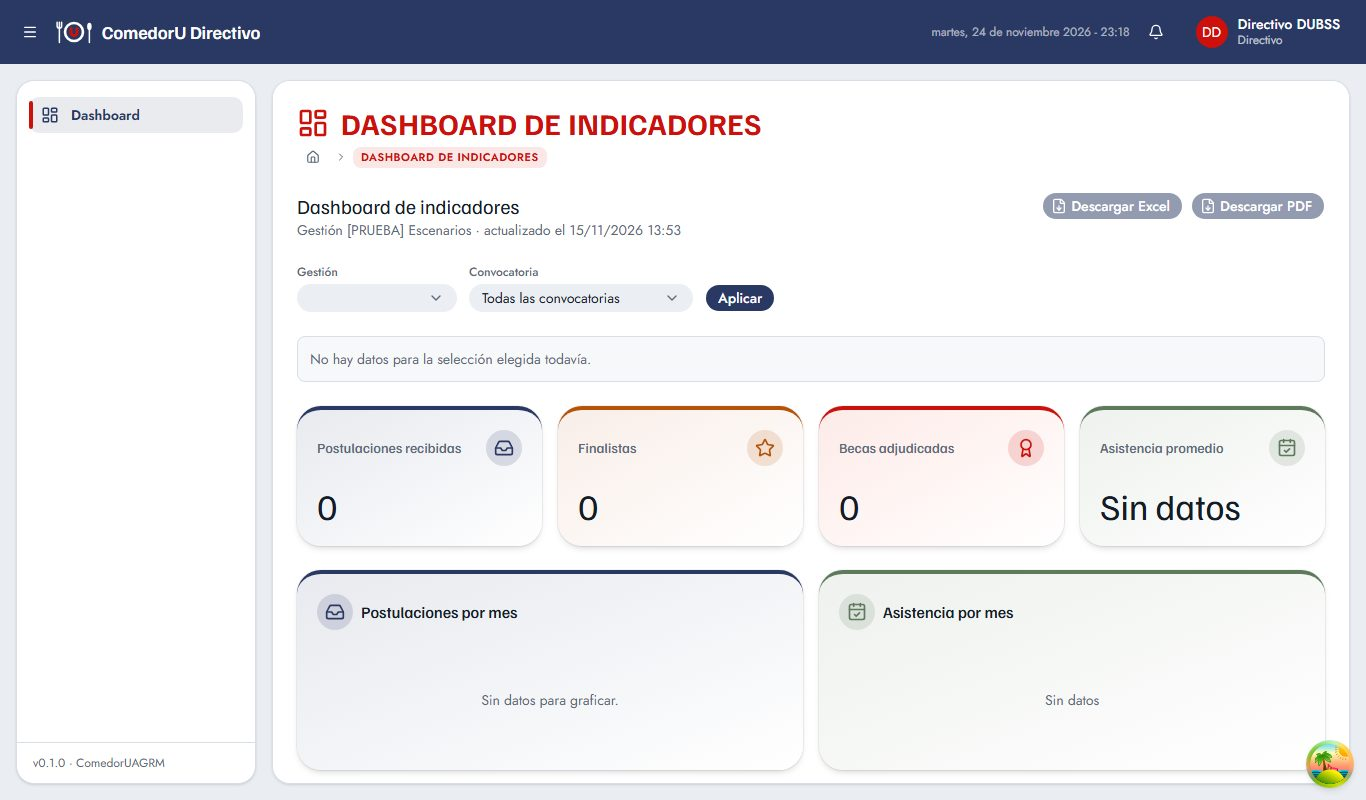
\includegraphics[width=0.93\linewidth,height=4.8cm,keepaspectratio]{images/189_CN_CU-12_A_inicial.jpg}}\vspace{2pt}\end{minipage}} \\
Resultado de prueba & {\textcolor{green!45!black}{\textbf{CORRECTO}}} \\
\end{longtable}
\endgroup
\addtocounter{table}{-1}
\vspace{-0.5\baselineskip}

\refstepcounter{table}\label{tab:cn_cu12_b}
\addcontentsline{lot}{table}{\protect\numberline{\thetable}CU-12. Visualizar dashboard de indicadores BI (indicadores)}
\noindent\textbf{Tabla~\thetable}\par\nopagebreak
\noindent\textit{CU-12. Visualizar dashboard de indicadores BI (indicadores)}\par\nopagebreak
\begingroup\footnotesize\linespread{1}\selectfont
\setlength{\LTleft}{0pt}\setlength{\LTright}{\fill}
\begin{longtable}{>{\raggedright\arraybackslash}p{3.6cm} >{\raggedright\arraybackslash}p{11.4cm}}
\toprule
\textbf{Campo} & \textbf{Contenido} \\
\midrule
\endfirsthead
\toprule
\textbf{Campo} & \textbf{Contenido} \\
\midrule
\endhead
\midrule
\multicolumn{2}{r}{\textit{Continúa en la siguiente página}} \\
\endfoot
\bottomrule
\multicolumn{2}{l}{\textit{Nota.} Elaboración propia a partir de la ejecución de la prueba.} \\
\endlastfoot
Nombre del caso de prueba & {CU-12. Visualizar dashboard de indicadores BI (indicadores)} \\
Descripción & {El directivo filtra por gestión y ve los indicadores, los gráficos y el análisis BI.} \\
Precondición & {Sesión del directivo.} \\
Datos de entrada & {Gestión «[PRUEBA] 2026-II», todas las convocatorias.} \\
Condición de ejecución & {No aplica} \\
Captura de imagen inicial & {\begin{minipage}[t]{\linewidth}\strut\par\vspace{3pt}\fcolorbox{gray}{white}{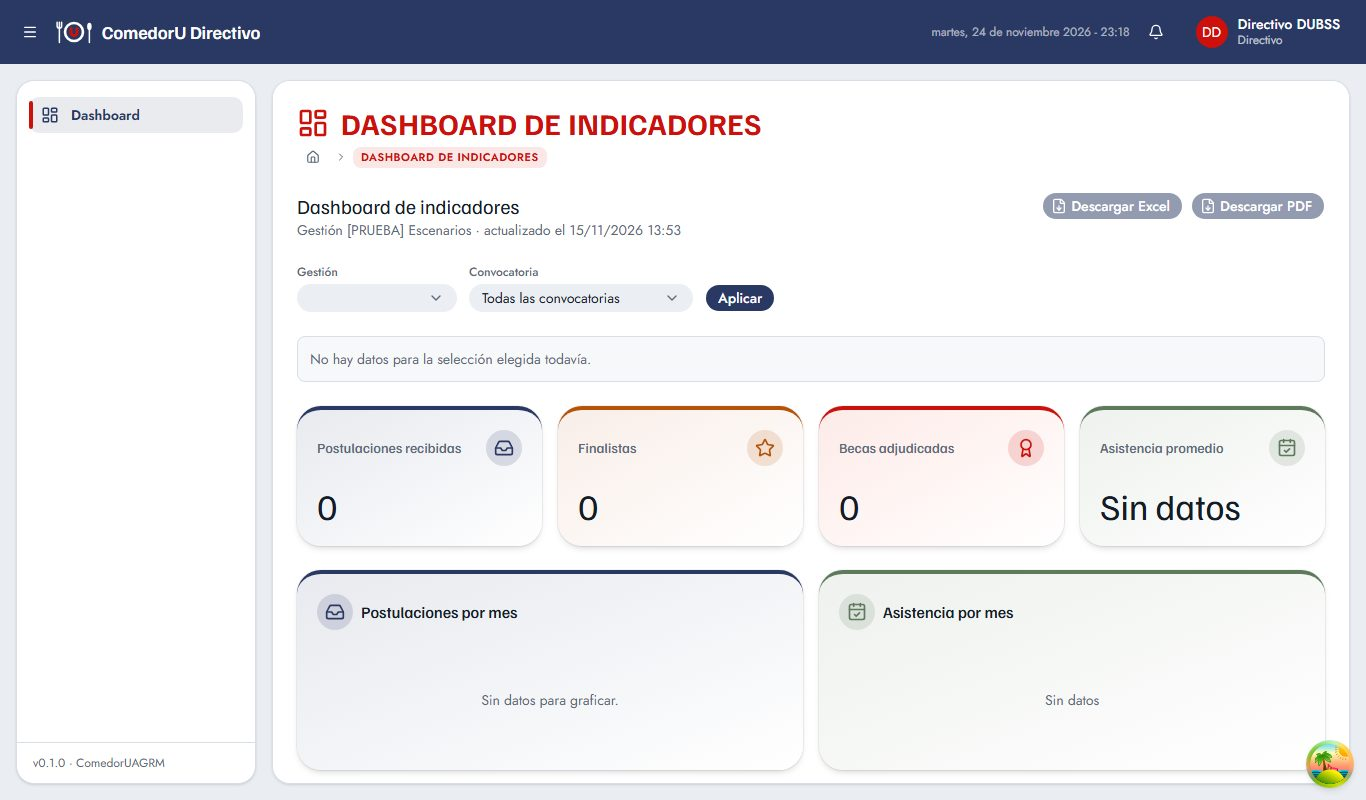
\includegraphics[width=0.93\linewidth,height=4.8cm,keepaspectratio]{images/190_CN_CU-12_B_inicial.jpg}}\vspace{2pt}\end{minipage}} \\
Pasos & {1. Abrir el selector «Gestión» y elegir «[PRUEBA] 2026-II».\newline 2. Pulsar «Aplicar».\newline 3. Desplazarse hasta «Análisis BI».} \\
Resultado esperado & {Se actualizan los cuatro indicadores y los gráficos, y aparece el análisis BI.} \\
Resultado obtenido & {Postulaciones recibidas 129, finalistas 39, becas adjudicadas 6, asistencia promedio «Sin datos»; gráfico de postulaciones por mes (jul a nov 2026) y sección «Análisis BI» con embudo y postulaciones por facultad.} \\
Captura de imagen final & {\begin{minipage}[t]{\linewidth}\strut\par\vspace{3pt}\fcolorbox{gray}{white}{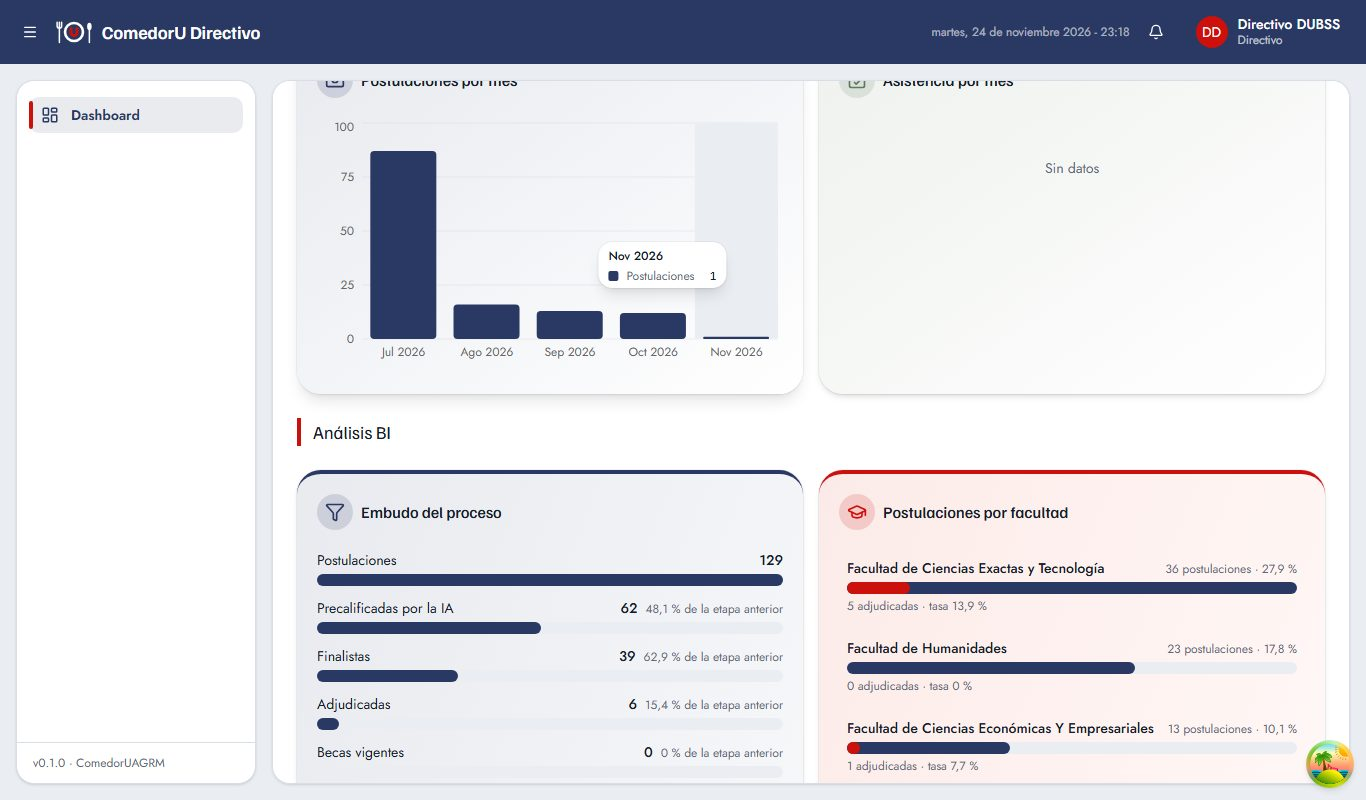
\includegraphics[width=0.93\linewidth,height=4.8cm,keepaspectratio]{images/191_CN_CU-12_B_analisis_bi.jpg}}\vspace{2pt}\par\vspace{3pt}\fcolorbox{gray}{white}{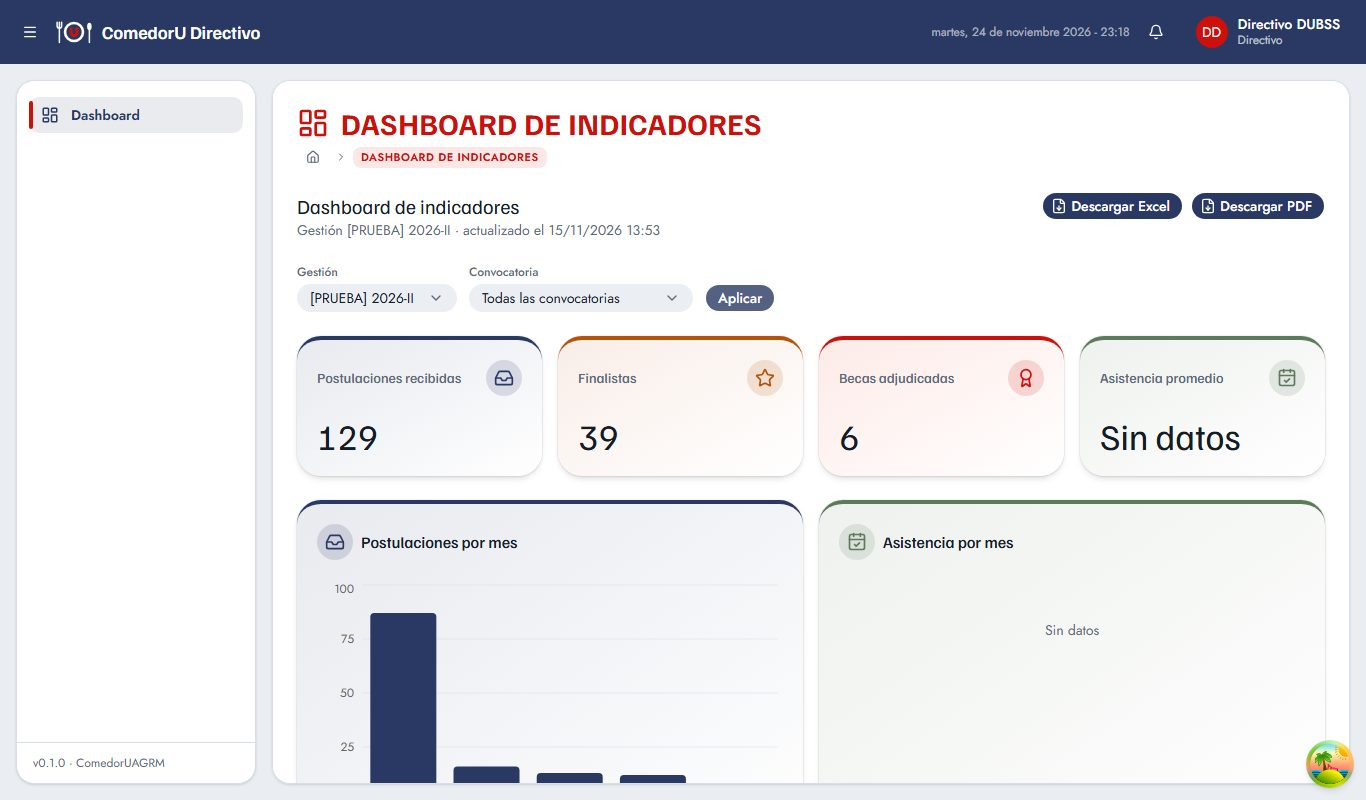
\includegraphics[width=0.93\linewidth,height=4.8cm,keepaspectratio]{images/192_CN_CU-12_B_final.jpg}}\vspace{2pt}\end{minipage}} \\
Resultado de prueba & {\textcolor{green!45!black}{\textbf{CORRECTO}}} \\
\end{longtable}
\endgroup
\addtocounter{table}{-1}
\vspace{-0.5\baselineskip}

\refstepcounter{table}\label{tab:cn_cu12_c}
\addcontentsline{lot}{table}{\protect\numberline{\thetable}CU-12. Visualizar dashboard de indicadores BI (exportación a PDF)}
\noindent\textbf{Tabla~\thetable}\par\nopagebreak
\noindent\textit{CU-12. Visualizar dashboard de indicadores BI (exportación a PDF)}\par\nopagebreak
\begingroup\footnotesize\linespread{1}\selectfont
\setlength{\LTleft}{0pt}\setlength{\LTright}{\fill}
\begin{longtable}{>{\raggedright\arraybackslash}p{3.6cm} >{\raggedright\arraybackslash}p{11.4cm}}
\toprule
\textbf{Campo} & \textbf{Contenido} \\
\midrule
\endfirsthead
\toprule
\textbf{Campo} & \textbf{Contenido} \\
\midrule
\endhead
\midrule
\multicolumn{2}{r}{\textit{Continúa en la siguiente página}} \\
\endfoot
\bottomrule
\multicolumn{2}{l}{\textit{Nota.} Elaboración propia a partir de la ejecución de la prueba.} \\
\endlastfoot
Nombre del caso de prueba & {CU-12. Visualizar dashboard de indicadores BI (exportación a PDF)} \\
Descripción & {El directivo descarga un PDF con lo que ve en pantalla.} \\
Precondición & {Gestión «[PRUEBA] 2026-II» aplicada.} \\
Datos de entrada & {Botón «Descargar PDF».} \\
Condición de ejecución & {No aplica} \\
Captura de imagen inicial & {\begin{minipage}[t]{\linewidth}\strut\par\vspace{3pt}\fcolorbox{gray}{white}{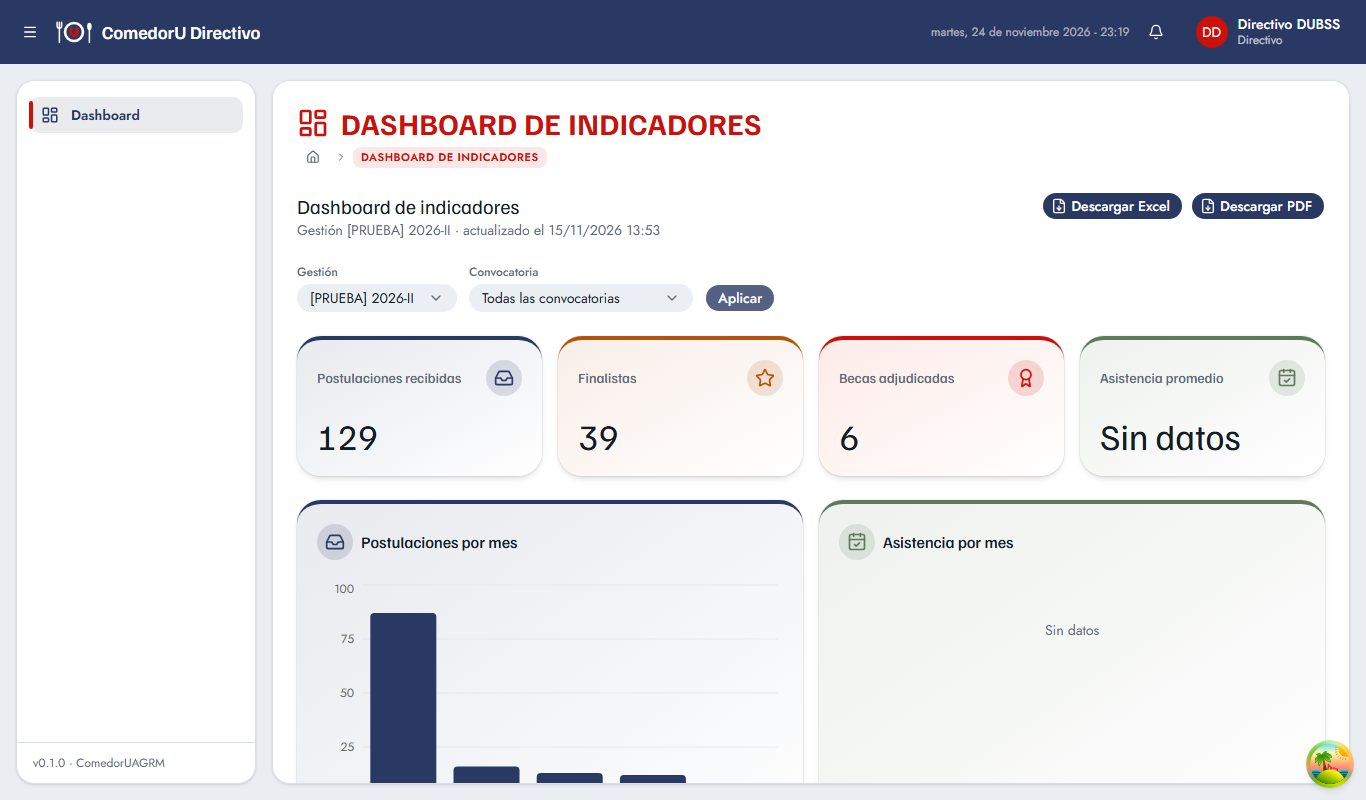
\includegraphics[width=0.93\linewidth,height=4.8cm,keepaspectratio]{images/193_CN_CU-12_C_inicial.jpg}}\vspace{2pt}\end{minipage}} \\
Pasos & {1. Aplicar la gestión «[PRUEBA] 2026-II».\newline 2. Pulsar «Descargar PDF».} \\
Resultado esperado & {Se descarga un PDF con los indicadores.} \\
Resultado obtenido & {Se descargó \texttt{indicadores-\allowbreak{}prueba-\allowbreak{}2026-\allowbreak{}ii-\allowbreak{}20261124.\allowbreak{}pdf} (310 237 bytes).} \\
Captura de imagen final & {\begin{minipage}[t]{\linewidth}\strut\par\vspace{3pt}\fcolorbox{gray}{white}{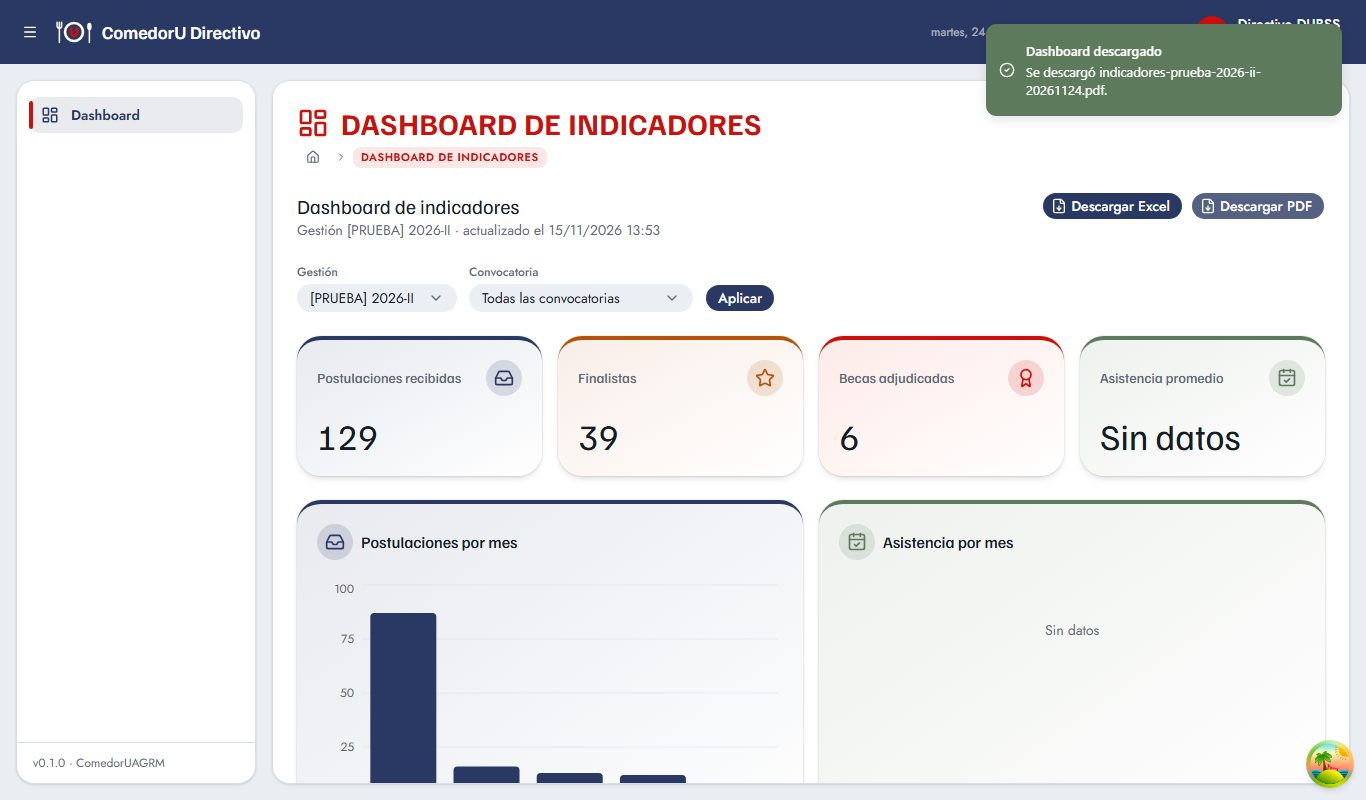
\includegraphics[width=0.93\linewidth,height=4.8cm,keepaspectratio]{images/194_CN_CU-12_C_final.jpg}}\vspace{2pt}\end{minipage}} \\
Resultado de prueba & {\textcolor{green!45!black}{\textbf{CORRECTO}}} \\
\end{longtable}
\endgroup
\addtocounter{table}{-1}
\vspace{-0.5\baselineskip}

\refstepcounter{table}\label{tab:cn_cu12_d}
\addcontentsline{lot}{table}{\protect\numberline{\thetable}CU-12. Visualizar dashboard de indicadores BI (control de acceso)}
\noindent\textbf{Tabla~\thetable}\par\nopagebreak
\noindent\textit{CU-12. Visualizar dashboard de indicadores BI (control de acceso)}\par\nopagebreak
\begingroup\footnotesize\linespread{1}\selectfont
\setlength{\LTleft}{0pt}\setlength{\LTright}{\fill}
\begin{longtable}{>{\raggedright\arraybackslash}p{3.6cm} >{\raggedright\arraybackslash}p{11.4cm}}
\toprule
\textbf{Campo} & \textbf{Contenido} \\
\midrule
\endfirsthead
\toprule
\textbf{Campo} & \textbf{Contenido} \\
\midrule
\endhead
\midrule
\multicolumn{2}{r}{\textit{Continúa en la siguiente página}} \\
\endfoot
\bottomrule
\multicolumn{2}{l}{\textit{Nota.} Elaboración propia a partir de la ejecución de la prueba.} \\
\endlastfoot
Nombre del caso de prueba & {CU-12. Visualizar dashboard de indicadores BI (control de acceso)} \\
Descripción & {Solo el directivo accede al dashboard.} \\
Precondición & {Sesión del administrador.} \\
Datos de entrada & {Ruta \texttt{/\allowbreak{}dashboard}.} \\
Condición de ejecución & {No aplica} \\
Captura de imagen inicial & {No aplica: la prueba comprueba un estado y no tiene pantalla previa distinta de la final.} \\
Pasos & {1. Iniciar sesión como administrador.\newline 2. Escribir \texttt{/\allowbreak{}dashboard} en el navegador.} \\
Resultado esperado & {El sistema lo devuelve a su panel.} \\
Resultado obtenido & {La aplicación redirigió a \texttt{/\allowbreak{}panel}.} \\
Captura de imagen final & {\begin{minipage}[t]{\linewidth}\strut\par\vspace{3pt}\fcolorbox{gray}{white}{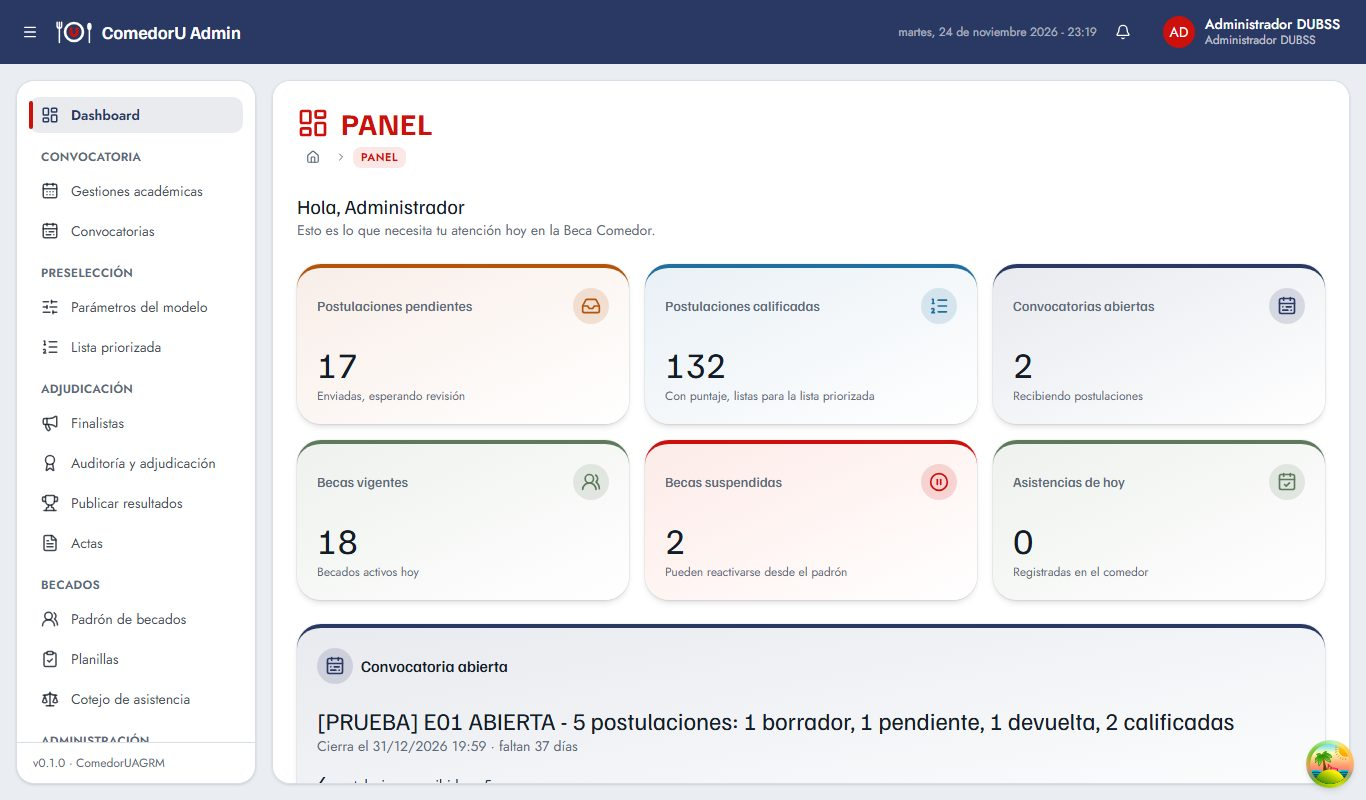
\includegraphics[width=0.93\linewidth,height=4.8cm,keepaspectratio]{images/195_CN_CU-12_D_final.jpg}}\vspace{2pt}\end{minipage}} \\
Resultado de prueba & {\textcolor{green!45!black}{\textbf{CORRECTO}}} \\
\end{longtable}
\endgroup
\addtocounter{table}{-1}
\vspace{-0.5\baselineskip}

\paragraph{CU-14. Gestionar usuarios y roles.}\label{sec:cn_cu14} 

\refstepcounter{table}\label{tab:cn_cu14_a}
\addcontentsline{lot}{table}{\protect\numberline{\thetable}CU-14. Gestionar usuarios y roles (alta de cuenta)}
\noindent\textbf{Tabla~\thetable}\par\nopagebreak
\noindent\textit{CU-14. Gestionar usuarios y roles (alta de cuenta)}\par\nopagebreak
\begingroup\footnotesize\linespread{1}\selectfont
\setlength{\LTleft}{0pt}\setlength{\LTright}{\fill}
\begin{longtable}{>{\raggedright\arraybackslash}p{3.6cm} >{\raggedright\arraybackslash}p{11.4cm}}
\toprule
\textbf{Campo} & \textbf{Contenido} \\
\midrule
\endfirsthead
\toprule
\textbf{Campo} & \textbf{Contenido} \\
\midrule
\endhead
\midrule
\multicolumn{2}{r}{\textit{Continúa en la siguiente página}} \\
\endfoot
\bottomrule
\multicolumn{2}{l}{\textit{Nota.} Elaboración propia a partir de la ejecución de la prueba.} \\
\endlastfoot
Nombre del caso de prueba & {CU-14. Gestionar usuarios y roles (alta de cuenta)} \\
Descripción & {El administrador crea una cuenta de personal; el sistema genera una contraseña temporal que se muestra una sola vez.} \\
Precondición & {Sesión del Administrador DUBSS. Pantalla \texttt{/\allowbreak{}usuarios/\allowbreak{}directivos}.} \\
Datos de entrada & {Nombres «Rodrigo», apellidos «Suárez Melgar», CI y correo únicos generados para la prueba.} \\
Condición de ejecución & {No aplica} \\
Captura de imagen inicial & {\begin{minipage}[t]{\linewidth}\strut\par\vspace{3pt}\fcolorbox{gray}{white}{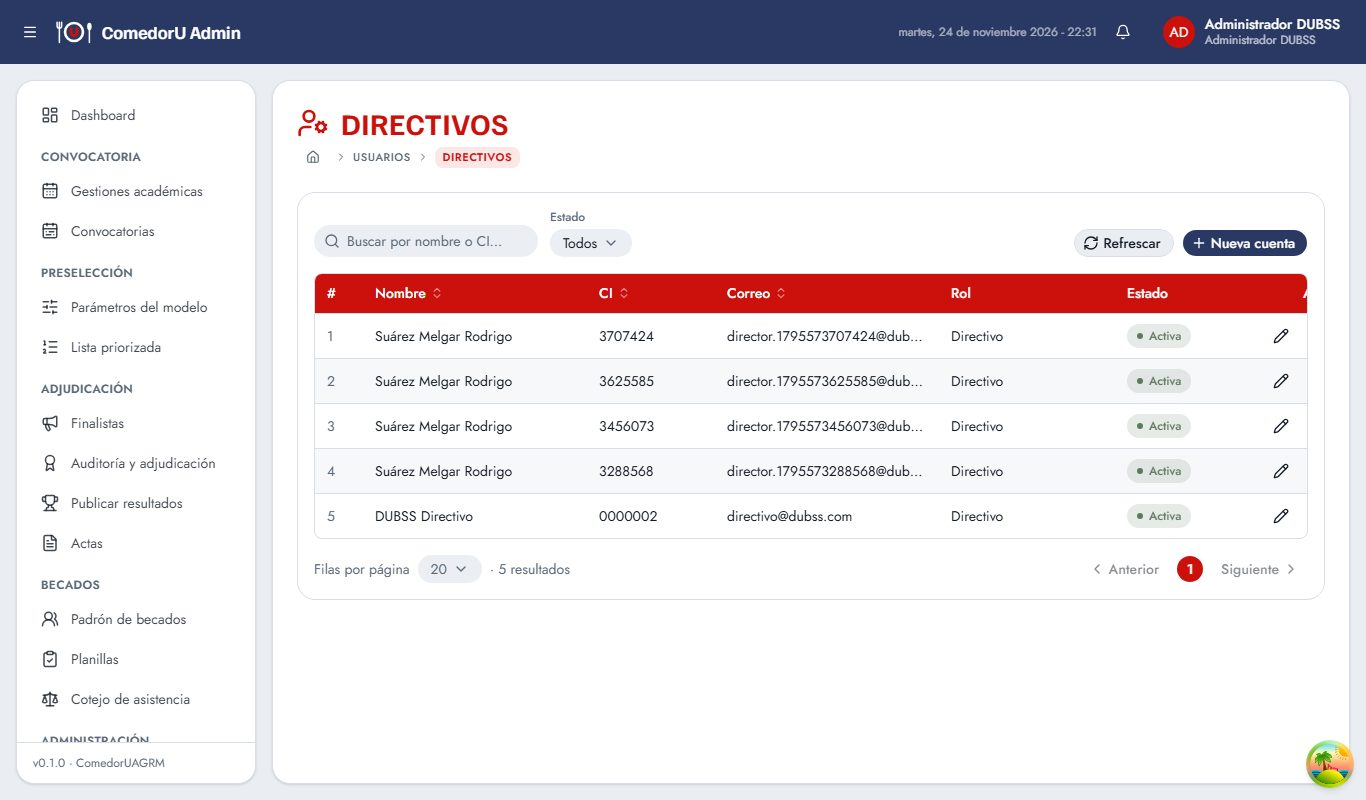
\includegraphics[width=0.93\linewidth,height=4.8cm,keepaspectratio]{images/196_CN_CU-14_A_inicial.jpg}}\vspace{2pt}\end{minipage}} \\
Pasos & {1. Abrir «Directivos» en el menú.\newline 2. Pulsar «Nueva cuenta» y completar el formulario.\newline 3. Pulsar «Crear cuenta» y copiar la contraseña temporal.\newline 4. Cerrar la sesión e iniciar sesión con la cuenta nueva y la contraseña temporal.} \\
Resultado esperado & {La cuenta se crea, se muestra una contraseña temporal una sola vez y con ella se puede entrar al módulo del rol.} \\
Resultado obtenido & {Apareció «Cuenta creada» con una contraseña temporal de 12 caracteres y el aviso «Esta contraseña no se volverá a mostrar». El inicio de sesión con esa contraseña llevó a \texttt{/\allowbreak{}dashboard}.} \\
Captura de imagen final & {\begin{minipage}[t]{\linewidth}\strut\par\vspace{3pt}\fcolorbox{gray}{white}{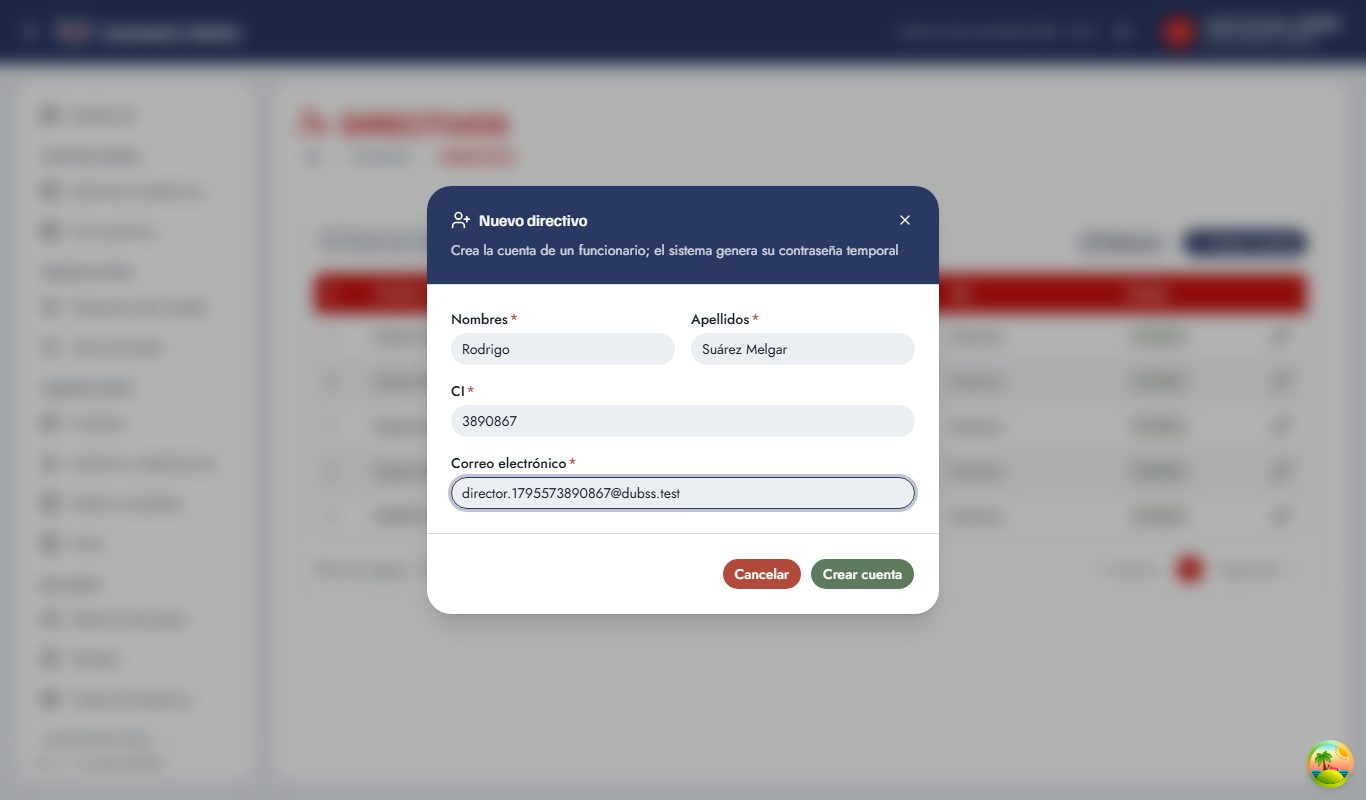
\includegraphics[width=0.93\linewidth,height=4.8cm,keepaspectratio]{images/197_CN_CU-14_A_formulario.jpg}}\vspace{2pt}\par\vspace{3pt}\fcolorbox{gray}{white}{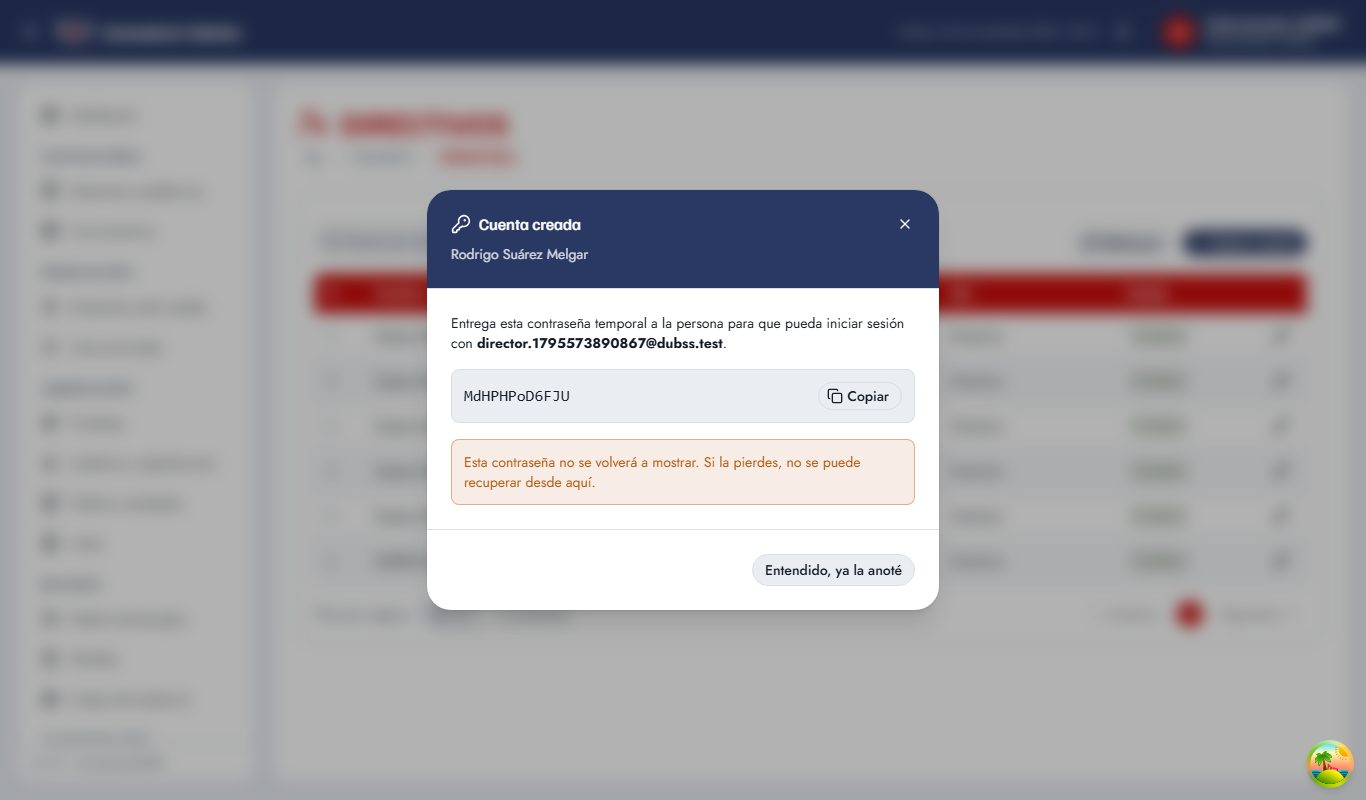
\includegraphics[width=0.93\linewidth,height=4.8cm,keepaspectratio]{images/198_CN_CU-14_A_final.jpg}}\vspace{2pt}\par\vspace{3pt}\fcolorbox{gray}{white}{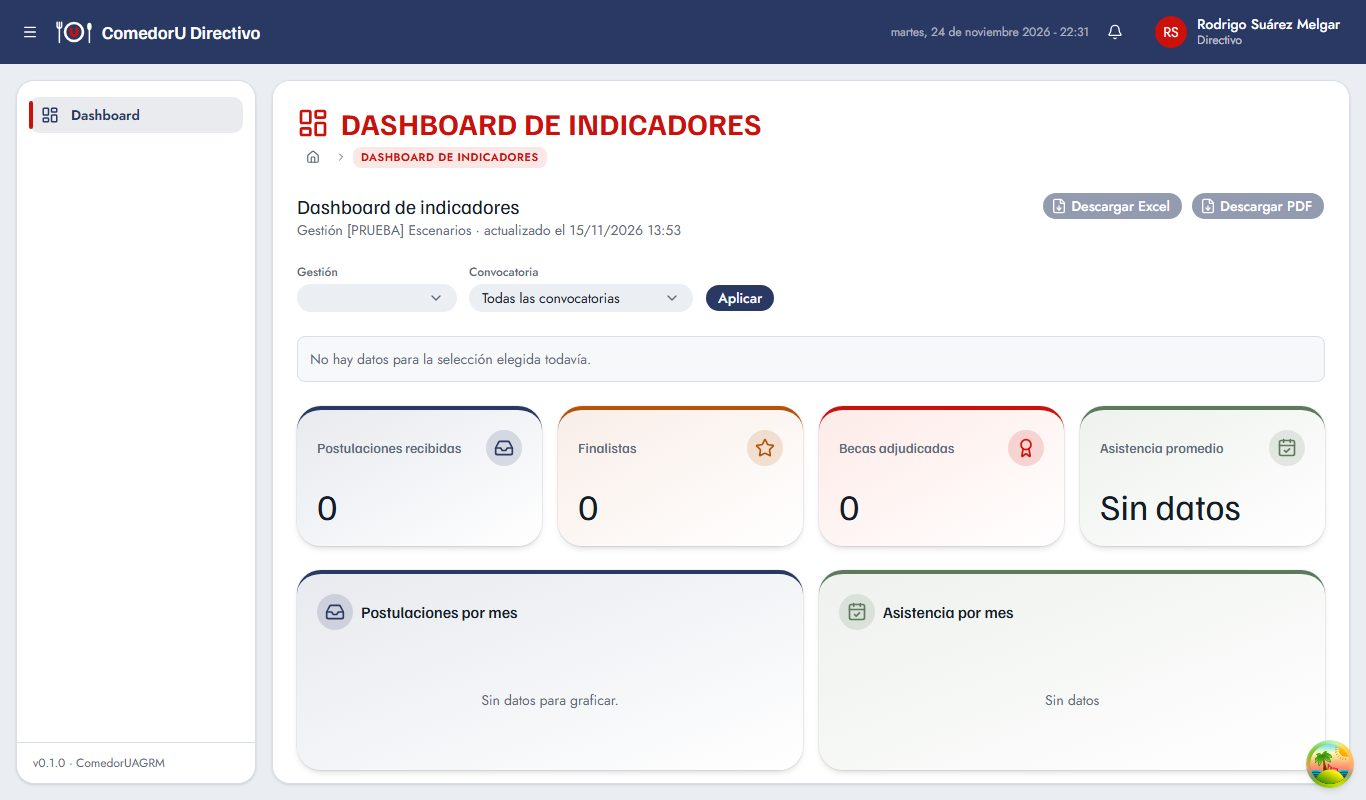
\includegraphics[width=0.93\linewidth,height=4.8cm,keepaspectratio]{images/199_CN_CU-14_A_login_temporal.jpg}}\vspace{2pt}\end{minipage}} \\
Resultado de prueba & {\textcolor{green!45!black}{\textbf{CORRECTO}}} \\
\end{longtable}
\endgroup
\addtocounter{table}{-1}
\vspace{-0.5\baselineskip}

\refstepcounter{table}\label{tab:cn_cu14_b}
\addcontentsline{lot}{table}{\protect\numberline{\thetable}CU-14. Gestionar usuarios y roles (CI duplicado)}
\noindent\textbf{Tabla~\thetable}\par\nopagebreak
\noindent\textit{CU-14. Gestionar usuarios y roles (CI duplicado)}\par\nopagebreak
\begingroup\footnotesize\linespread{1}\selectfont
\setlength{\LTleft}{0pt}\setlength{\LTright}{\fill}
\begin{longtable}{>{\raggedright\arraybackslash}p{3.6cm} >{\raggedright\arraybackslash}p{11.4cm}}
\toprule
\textbf{Campo} & \textbf{Contenido} \\
\midrule
\endfirsthead
\toprule
\textbf{Campo} & \textbf{Contenido} \\
\midrule
\endhead
\midrule
\multicolumn{2}{r}{\textit{Continúa en la siguiente página}} \\
\endfoot
\bottomrule
\multicolumn{2}{l}{\textit{Nota.} Elaboración propia a partir de la ejecución de la prueba.} \\
\endlastfoot
Nombre del caso de prueba & {CU-14. Gestionar usuarios y roles (CI duplicado)} \\
Descripción & {El sistema impide crear una cuenta con un CI que ya existe.} \\
Precondición & {Existe el directivo con CI 0000002.} \\
Datos de entrada & {CI «0000002», nombres «Otro», apellidos «Duplicado», correo nuevo.} \\
Condición de ejecución & {No aplica} \\
Captura de imagen inicial & {\begin{minipage}[t]{\linewidth}\strut\par\vspace{3pt}\fcolorbox{gray}{white}{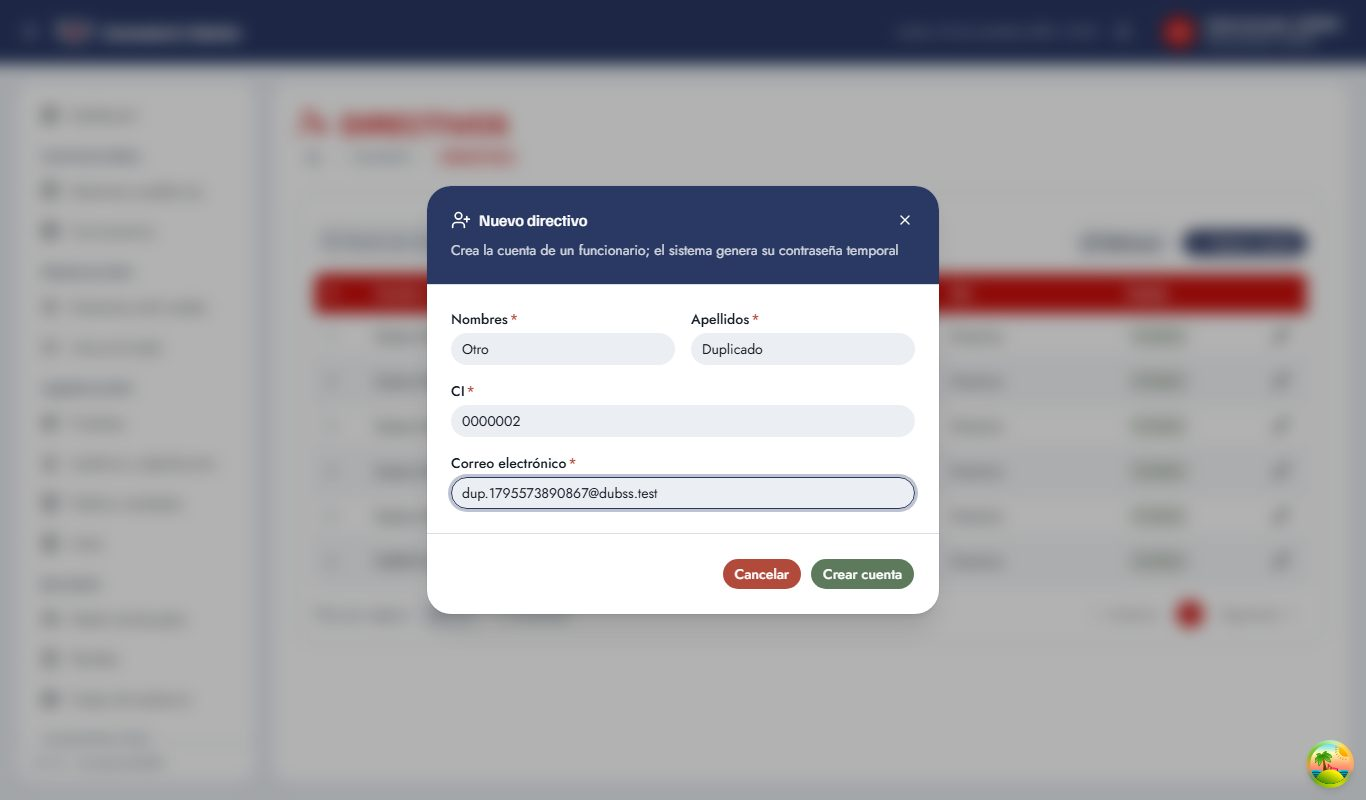
\includegraphics[width=0.93\linewidth,height=4.8cm,keepaspectratio]{images/200_CN_CU-14_B_inicial.jpg}}\vspace{2pt}\end{minipage}} \\
Pasos & {1. Abrir «Nueva cuenta» en \texttt{/\allowbreak{}usuarios/\allowbreak{}directivos}.\newline 2. Escribir el CI repetido y los demás datos.\newline 3. Pulsar «Crear cuenta».} \\
Resultado esperado & {No se crea la cuenta y se indica que el CI ya existe.} \\
Resultado obtenido & {El campo CI quedó marcado con «Ya existe una cuenta con ese CI» y el formulario siguió abierto.} \\
Captura de imagen final & {\begin{minipage}[t]{\linewidth}\strut\par\vspace{3pt}\fcolorbox{gray}{white}{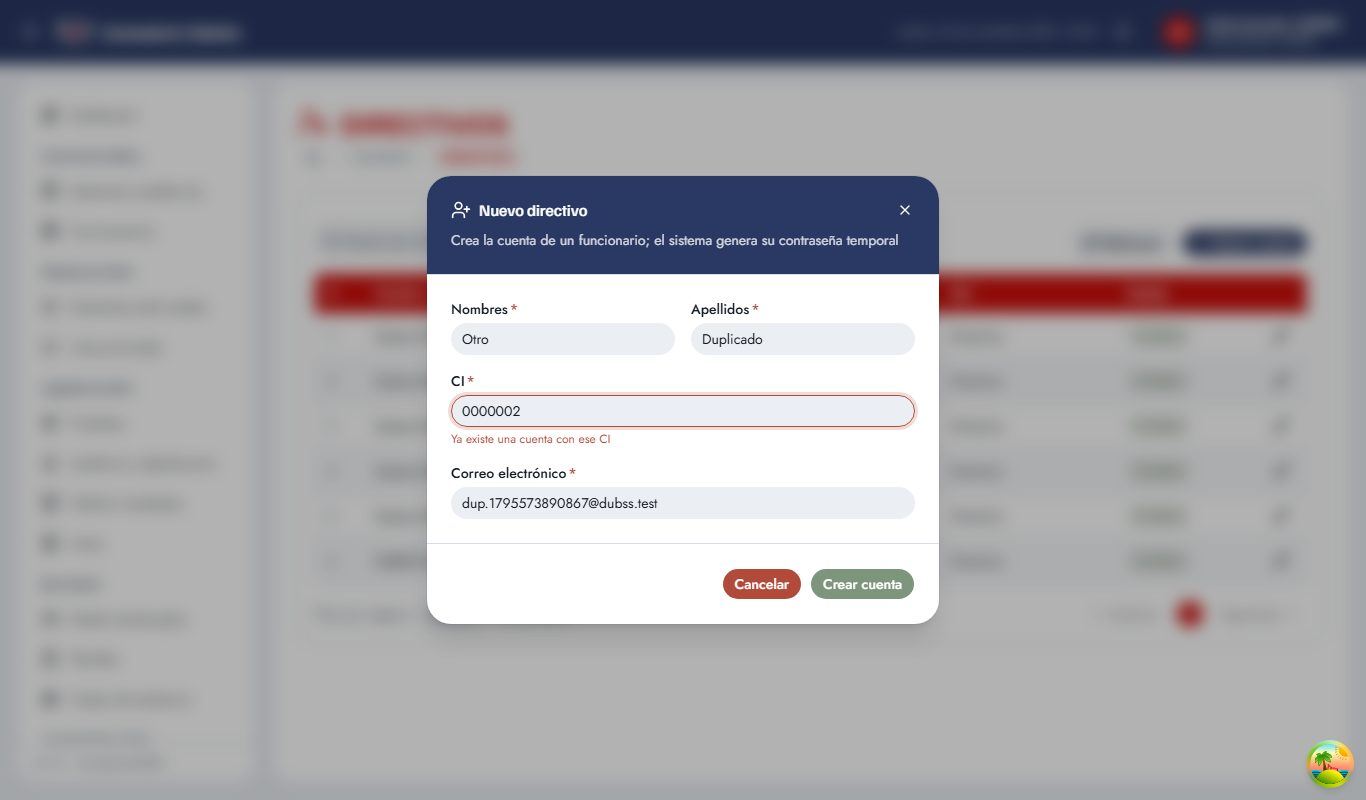
\includegraphics[width=0.93\linewidth,height=4.8cm,keepaspectratio]{images/201_CN_CU-14_B_final.jpg}}\vspace{2pt}\end{minipage}} \\
Resultado de prueba & {\textcolor{green!45!black}{\textbf{CORRECTO}}} \\
\end{longtable}
\endgroup
\addtocounter{table}{-1}
\vspace{-0.5\baselineskip}

\refstepcounter{table}\label{tab:cn_cu14_c}
\addcontentsline{lot}{table}{\protect\numberline{\thetable}CU-14. Gestionar usuarios y roles (desactivar cuenta)}
\noindent\textbf{Tabla~\thetable}\par\nopagebreak
\noindent\textit{CU-14. Gestionar usuarios y roles (desactivar cuenta)}\par\nopagebreak
\begingroup\footnotesize\linespread{1}\selectfont
\setlength{\LTleft}{0pt}\setlength{\LTright}{\fill}
\begin{longtable}{>{\raggedright\arraybackslash}p{3.6cm} >{\raggedright\arraybackslash}p{11.4cm}}
\toprule
\textbf{Campo} & \textbf{Contenido} \\
\midrule
\endfirsthead
\toprule
\textbf{Campo} & \textbf{Contenido} \\
\midrule
\endhead
\midrule
\multicolumn{2}{r}{\textit{Continúa en la siguiente página}} \\
\endfoot
\bottomrule
\multicolumn{2}{l}{\textit{Nota.} Elaboración propia a partir de la ejecución de la prueba.} \\
\endlastfoot
Nombre del caso de prueba & {CU-14. Gestionar usuarios y roles (desactivar cuenta)} \\
Descripción & {El administrador desactiva una cuenta; esa persona pierde el acceso.} \\
Precondición & {Cuenta creada en el caso A, activa.} \\
Datos de entrada & {Cuenta de «Rodrigo Suárez Melgar»; después, su correo y la contraseña temporal.} \\
Condición de ejecución & {No aplica} \\
Captura de imagen inicial & {\begin{minipage}[t]{\linewidth}\strut\par\vspace{3pt}\fcolorbox{gray}{white}{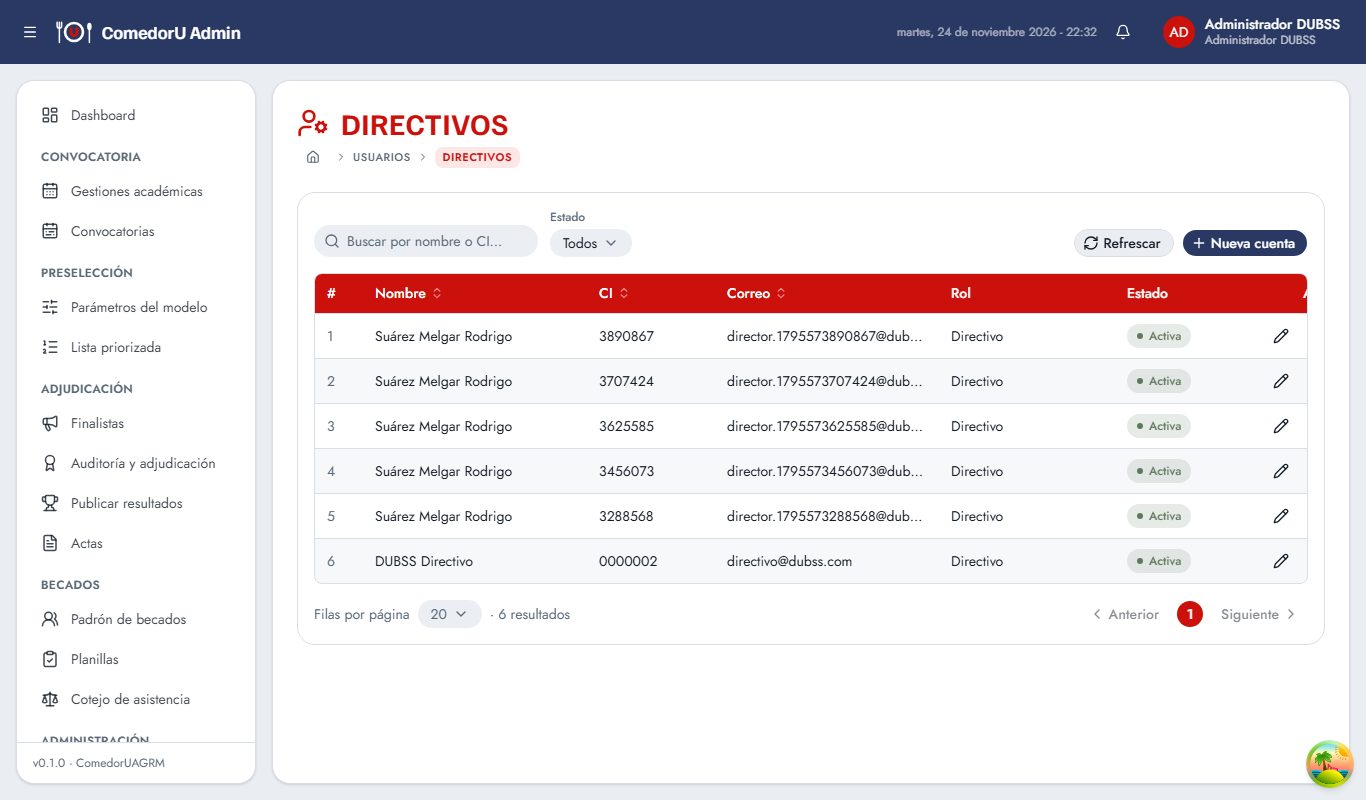
\includegraphics[width=0.93\linewidth,height=4.8cm,keepaspectratio]{images/202_CN_CU-14_C_inicial.jpg}}\vspace{2pt}\end{minipage}} \\
Pasos & {1. En \texttt{/\allowbreak{}usuarios/\allowbreak{}directivos} pulsar «Desactivar» en la fila de la cuenta.\newline 2. Confirmar en la ventana «¿Desactivar cuenta?».\newline 3. Cerrar la sesión e intentar iniciar sesión con esa cuenta.} \\
Resultado esperado & {La cuenta queda «Desactivada» y el inicio de sesión se rechaza.} \\
Resultado obtenido & {La fila pasó a estado «Desactivada». Al intentar entrar se mostró «Tu cuenta está desactivada.» y se permaneció en \texttt{/\allowbreak{}login}.} \\
Captura de imagen final & {\begin{minipage}[t]{\linewidth}\strut\par\vspace{3pt}\fcolorbox{gray}{white}{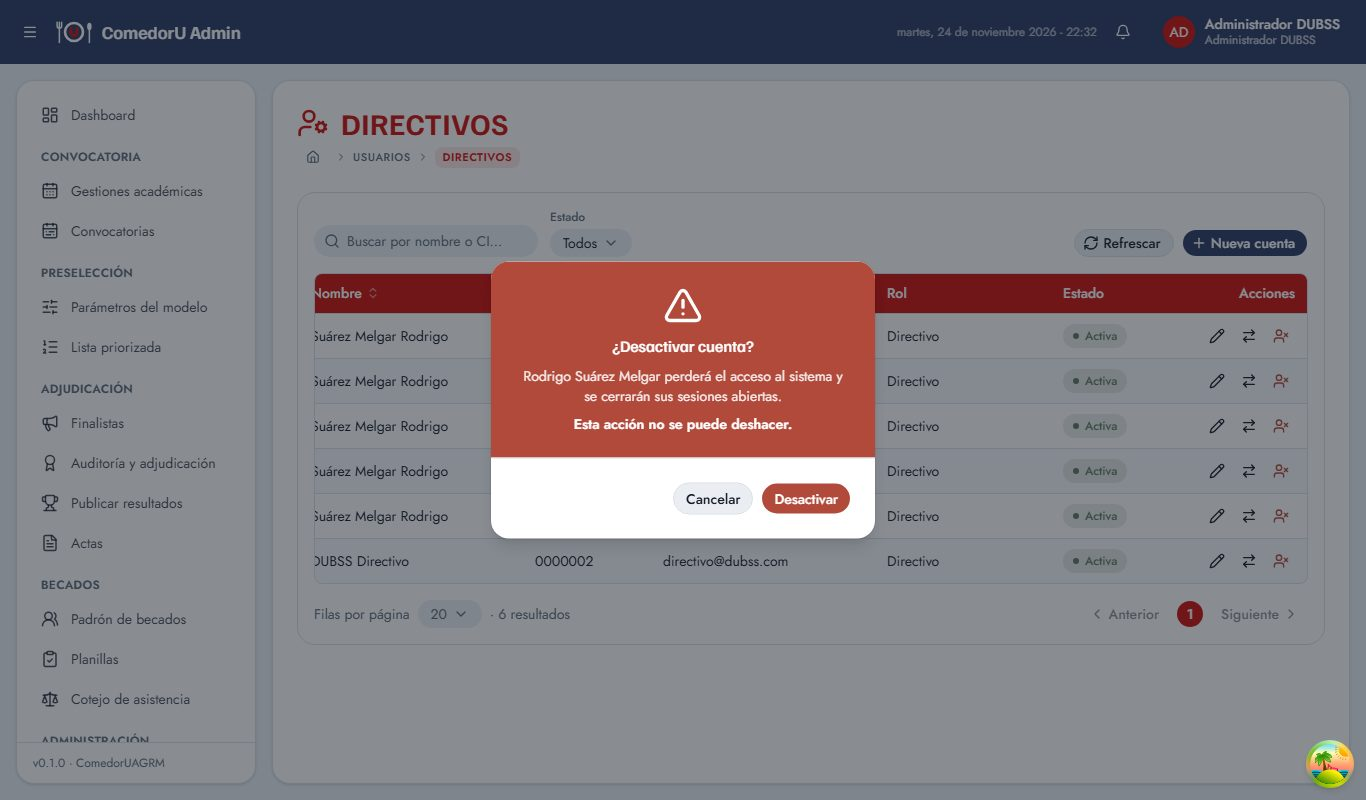
\includegraphics[width=0.93\linewidth,height=4.8cm,keepaspectratio]{images/203_CN_CU-14_C_confirmacion.jpg}}\vspace{2pt}\par\vspace{3pt}\fcolorbox{gray}{white}{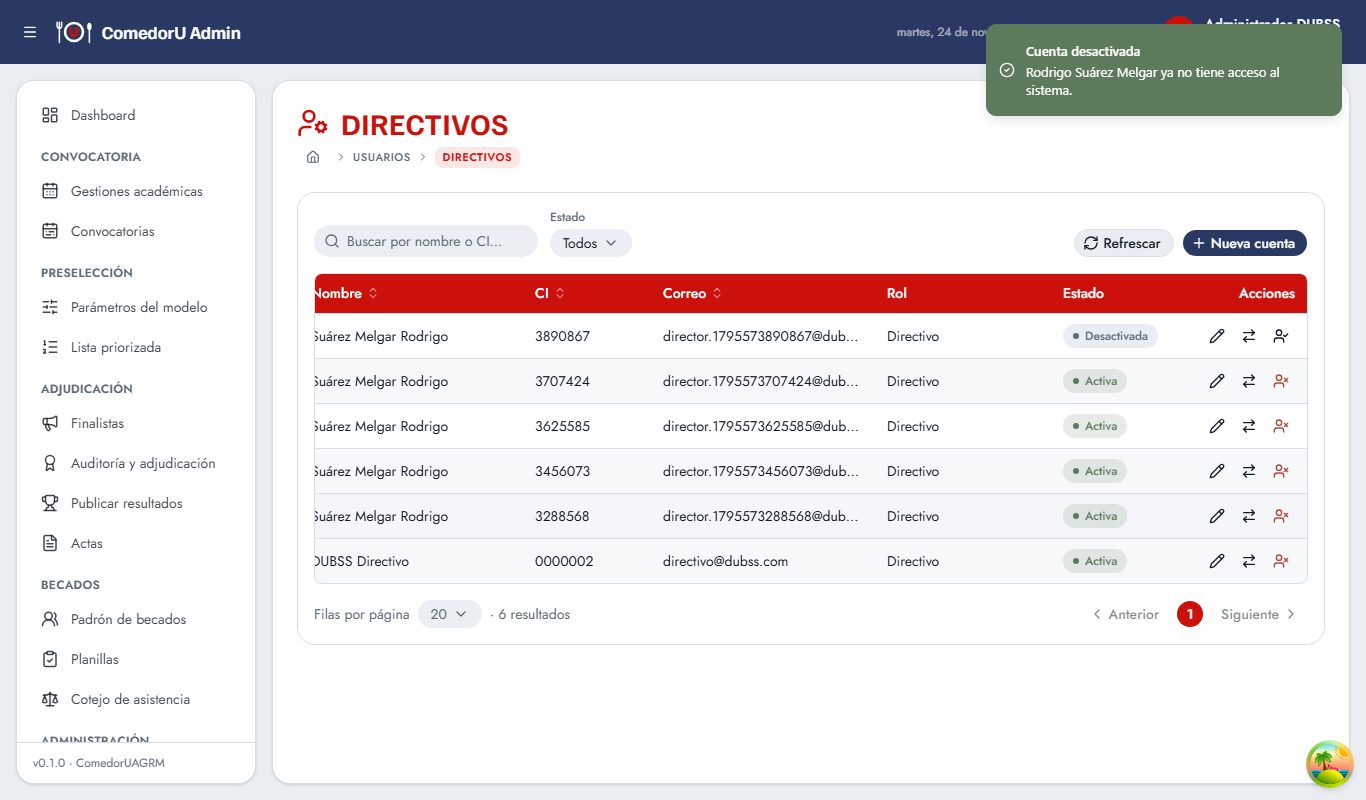
\includegraphics[width=0.93\linewidth,height=4.8cm,keepaspectratio]{images/204_CN_CU-14_C_final.jpg}}\vspace{2pt}\par\vspace{3pt}\fcolorbox{gray}{white}{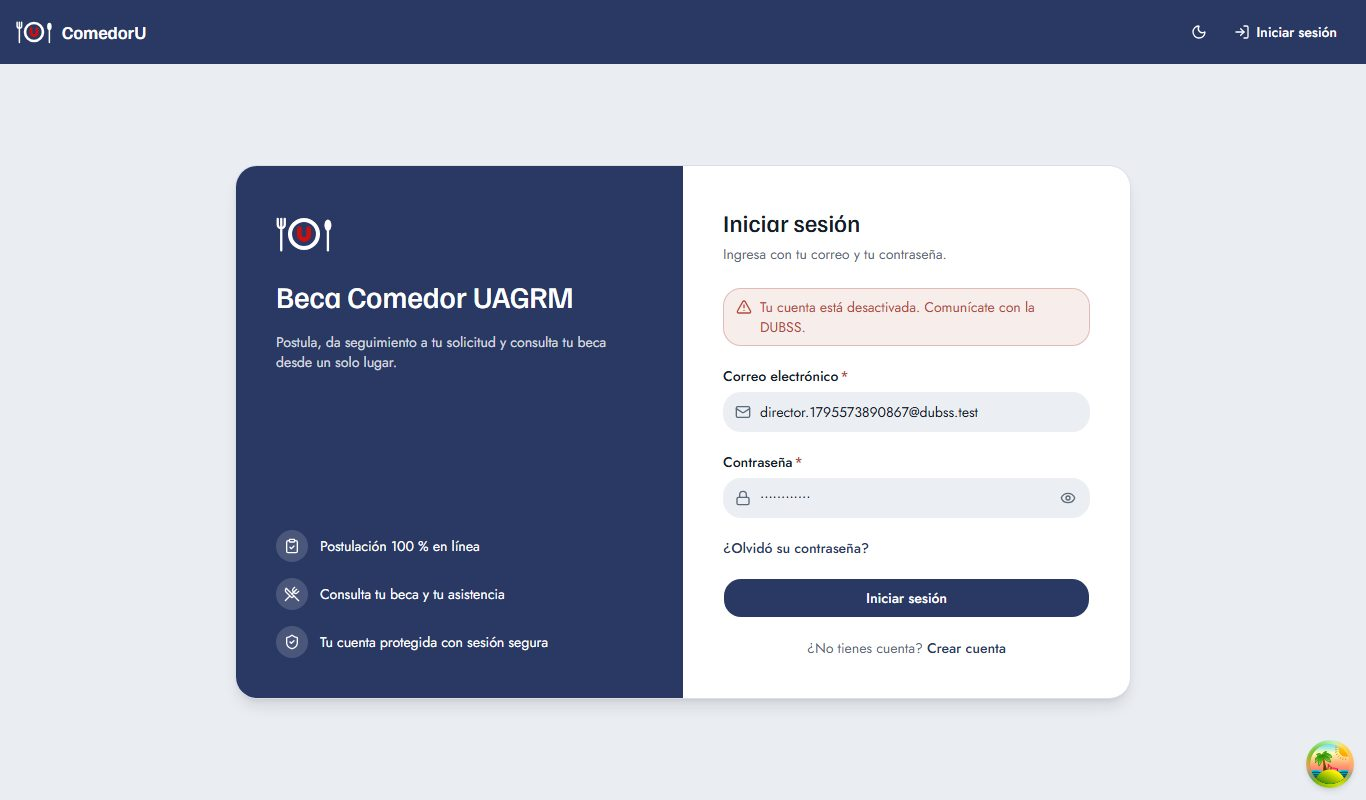
\includegraphics[width=0.93\linewidth,height=4.8cm,keepaspectratio]{images/205_CN_CU-14_C_login_desactivada.jpg}}\vspace{2pt}\end{minipage}} \\
Resultado de prueba & {\textcolor{green!45!black}{\textbf{CORRECTO}}} \\
\end{longtable}
\endgroup
\addtocounter{table}{-1}
\vspace{-0.5\baselineskip}

\paragraph{CU-15. Recuperar contraseña y gestionar perfil.}\label{sec:cn_cu15} 

\refstepcounter{table}\label{tab:cn_cu15_a}
\addcontentsline{lot}{table}{\protect\numberline{\thetable}CU-15. Recuperar contraseña y gestionar perfil (recuperación)}
\noindent\textbf{Tabla~\thetable}\par\nopagebreak
\noindent\textit{CU-15. Recuperar contraseña y gestionar perfil (recuperación)}\par\nopagebreak
\begingroup\footnotesize\linespread{1}\selectfont
\setlength{\LTleft}{0pt}\setlength{\LTright}{\fill}
\begin{longtable}{>{\raggedright\arraybackslash}p{3.6cm} >{\raggedright\arraybackslash}p{11.4cm}}
\toprule
\textbf{Campo} & \textbf{Contenido} \\
\midrule
\endfirsthead
\toprule
\textbf{Campo} & \textbf{Contenido} \\
\midrule
\endhead
\midrule
\multicolumn{2}{r}{\textit{Continúa en la siguiente página}} \\
\endfoot
\bottomrule
\multicolumn{2}{l}{\textit{Nota.} Elaboración propia a partir de la ejecución de la prueba.} \\
\endlastfoot
Nombre del caso de prueba & {CU-15. Recuperar contraseña y gestionar perfil (recuperación)} \\
Descripción & {El usuario pide un enlace temporal, lo recibe por correo, define una contraseña nueva y entra con ella; el enlace sirve una sola vez.} \\
Precondición & {Cuenta de postulante creada para la prueba (registro previo). Mailpit activo en \texttt{http:/\allowbreak{}/\allowbreak{}localhost:8025}.} \\
Datos de entrada & {Correo de la cuenta, contraseña nueva «NuevaClave456» y su confirmación.} \\
Condición de ejecución & {No aplica} \\
Captura de imagen inicial & {\begin{minipage}[t]{\linewidth}\strut\par\vspace{3pt}\fcolorbox{gray}{white}{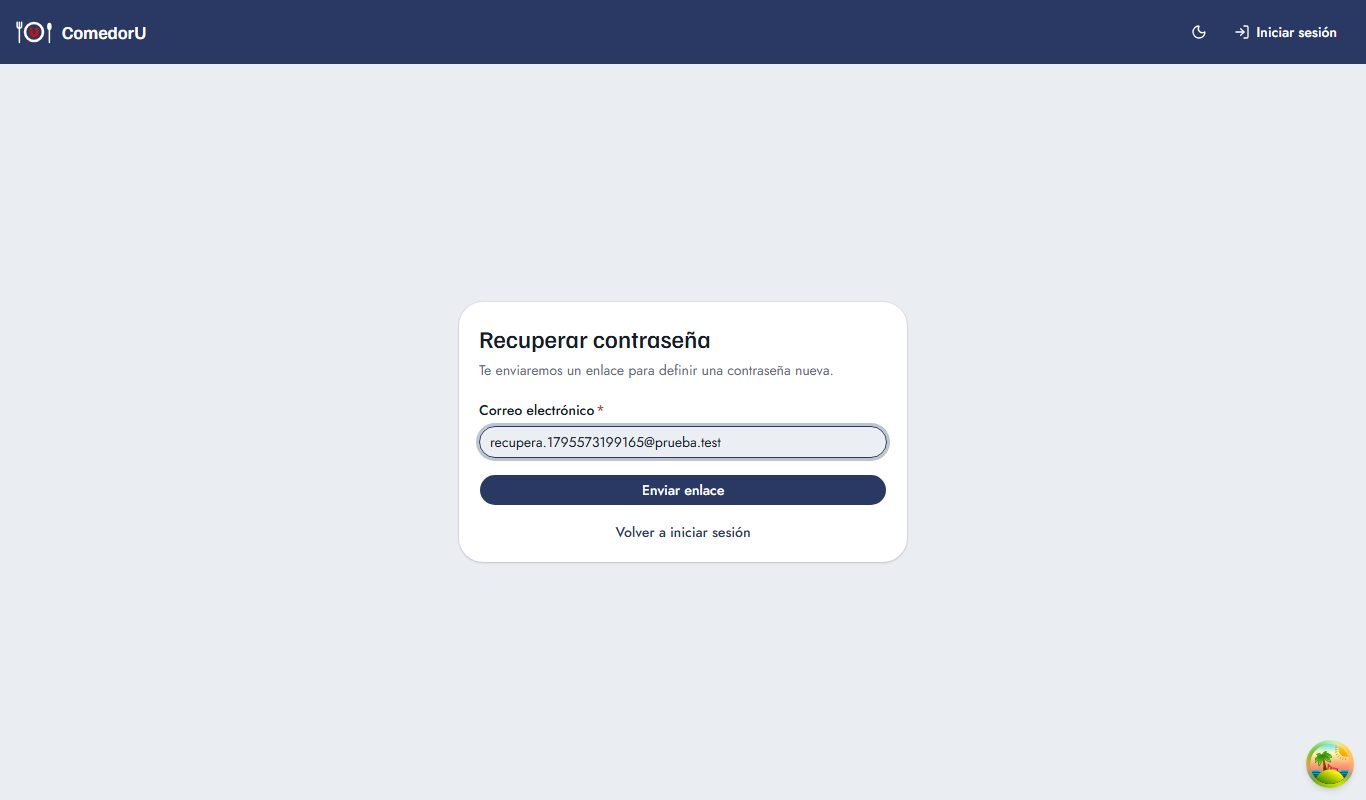
\includegraphics[width=0.93\linewidth,height=4.8cm,keepaspectratio]{images/206_CN_CU-15_A_inicial.jpg}}\vspace{2pt}\end{minipage}} \\
Pasos & {1. Abrir \texttt{/\allowbreak{}recuperar-\allowbreak{}contrasena}, escribir el correo y enviar.\newline 2. Abrir el correo recibido en Mailpit y copiar el enlace.\newline 3. Abrir el enlace, escribir y confirmar la contraseña nueva y pulsar «Guardar contraseña».\newline 4. Iniciar sesión con la contraseña nueva.} \\
Resultado esperado & {El sistema responde con un aviso neutro, envía el correo con el enlace, guarda la contraseña nueva y permite entrar con ella.} \\
Resultado obtenido & {Aviso: «Si la cuenta existe, enviamos un enlace al correo indicado. Vence en 60 minutos.». Mailpit recibió «Restablece tu contraseña de ComedorU». Tras guardar, la aplicación fue a \texttt{/\allowbreak{}login} y el inicio de sesión con la contraseña nueva llevó a \texttt{/\allowbreak{}panel}.} \\
Captura de imagen final & {\begin{minipage}[t]{\linewidth}\strut\par\vspace{3pt}\fcolorbox{gray}{white}{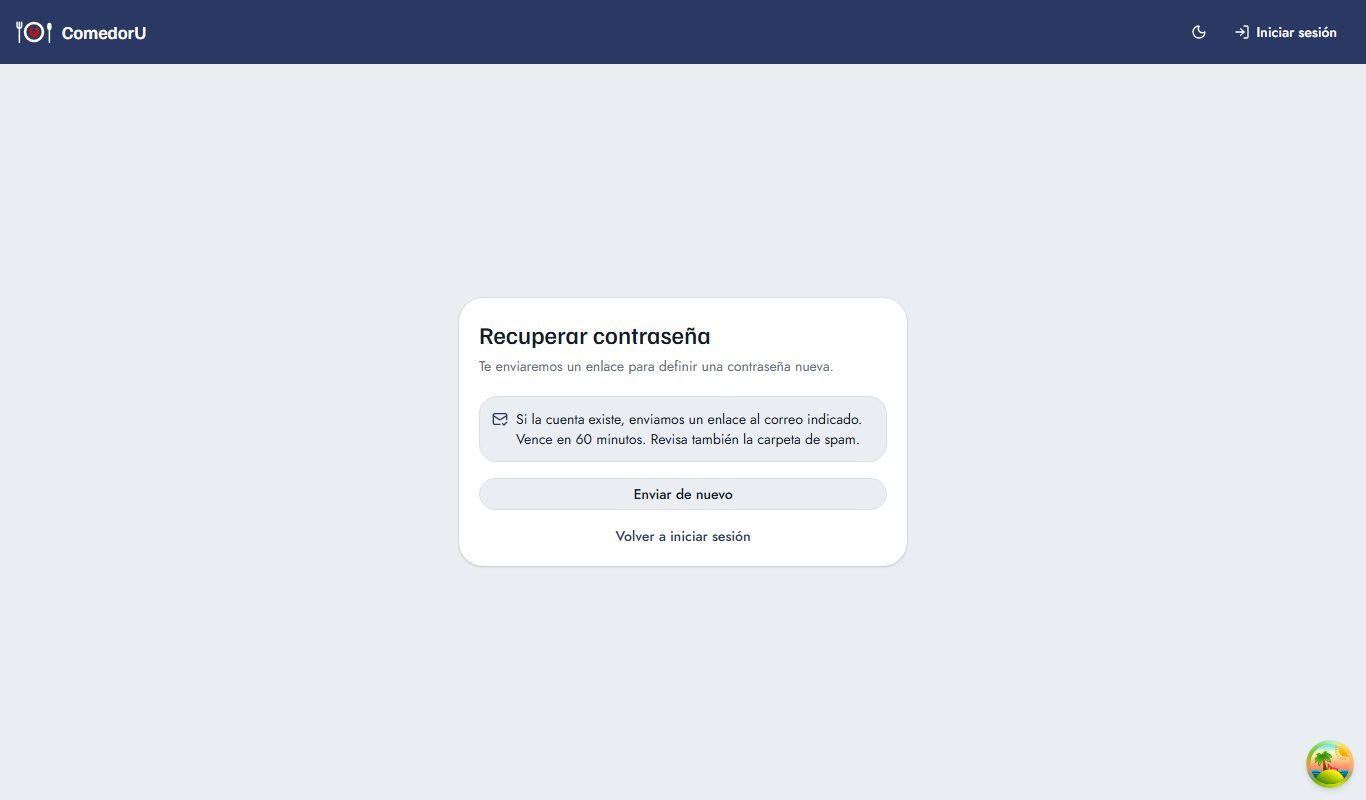
\includegraphics[width=0.93\linewidth,height=4.8cm,keepaspectratio]{images/207_CN_CU-15_A_aviso_neutro.jpg}}\vspace{2pt}\par\vspace{3pt}\fcolorbox{gray}{white}{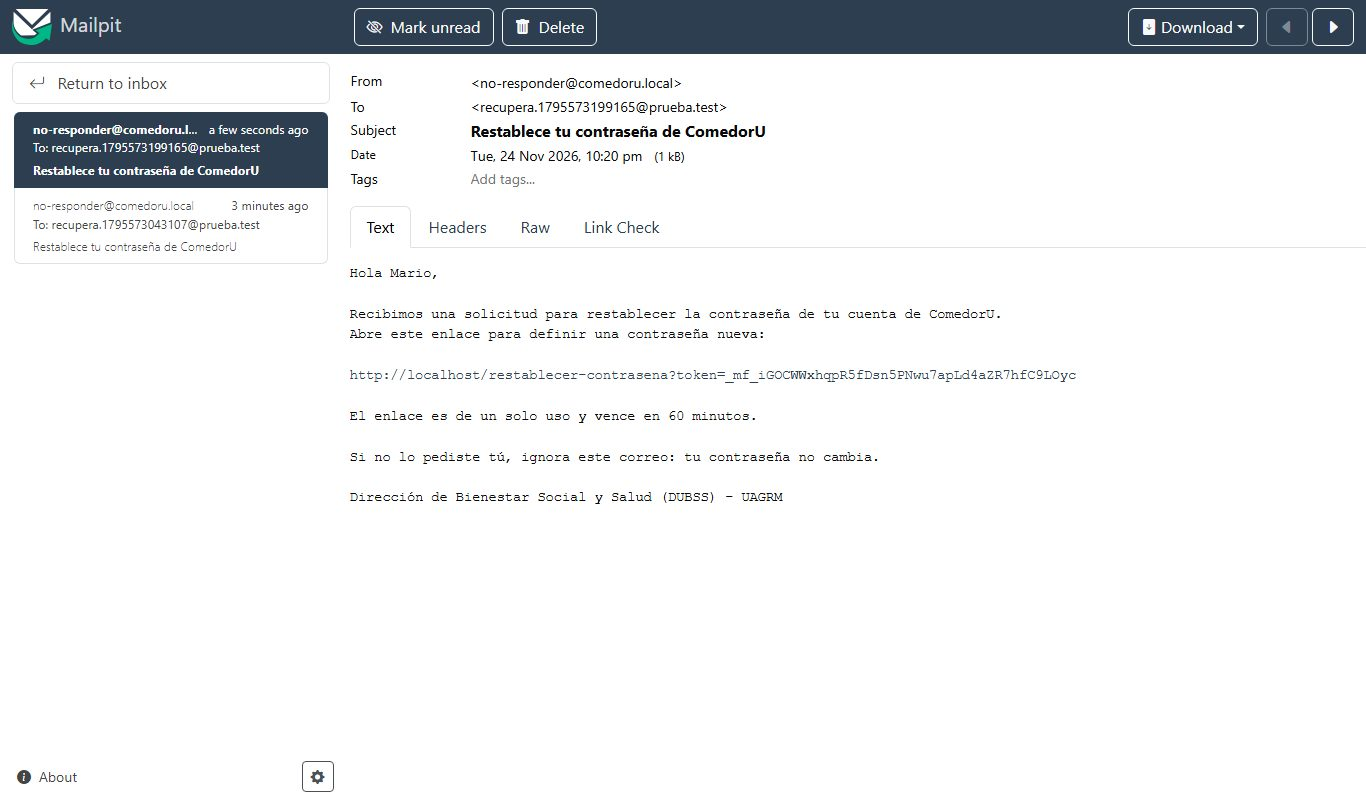
\includegraphics[width=0.93\linewidth,height=4.8cm,keepaspectratio]{images/208_CN_CU-15_A_correo_mailpit.jpg}}\vspace{2pt}\par\vspace{3pt}\fcolorbox{gray}{white}{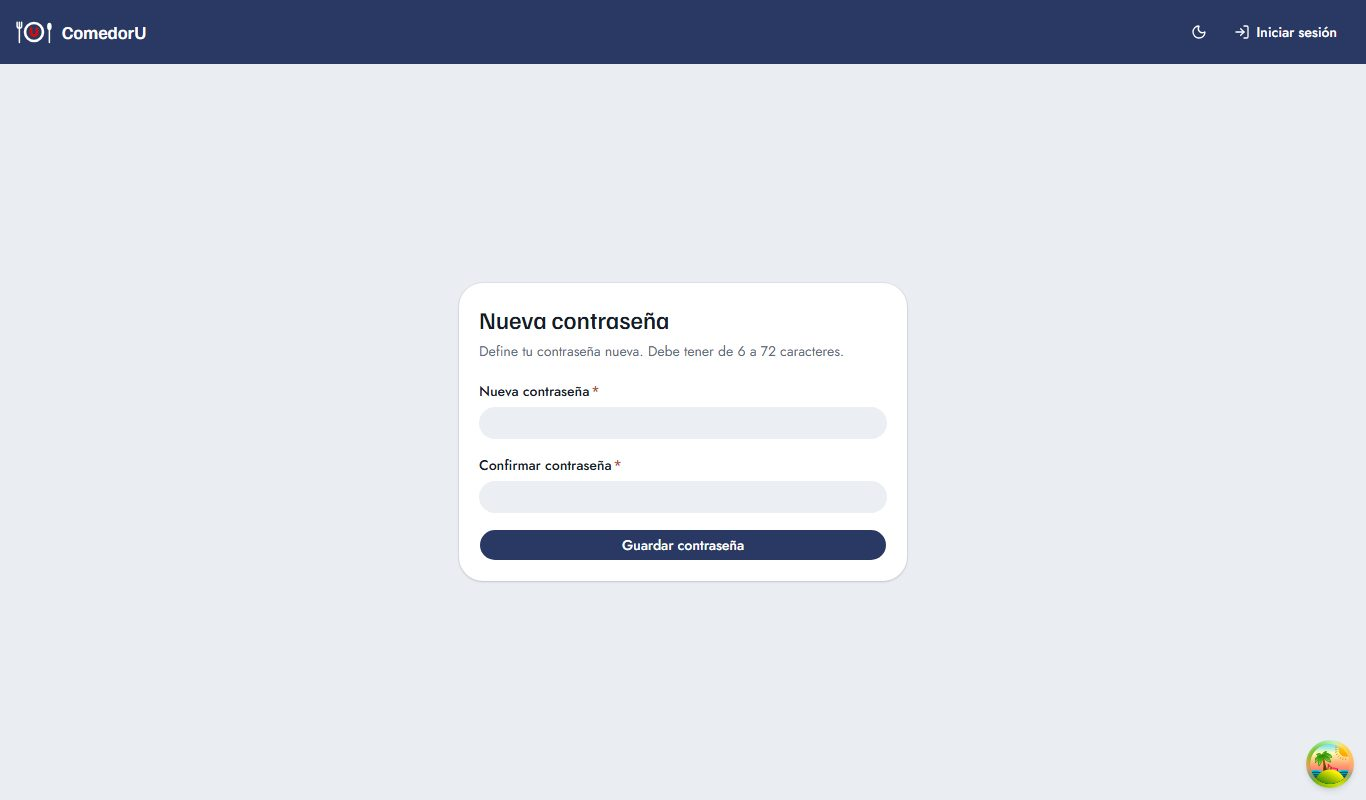
\includegraphics[width=0.93\linewidth,height=4.8cm,keepaspectratio]{images/209_CN_CU-15_A_formulario_restablecer.jpg}}\vspace{2pt}\par\vspace{3pt}\fcolorbox{gray}{white}{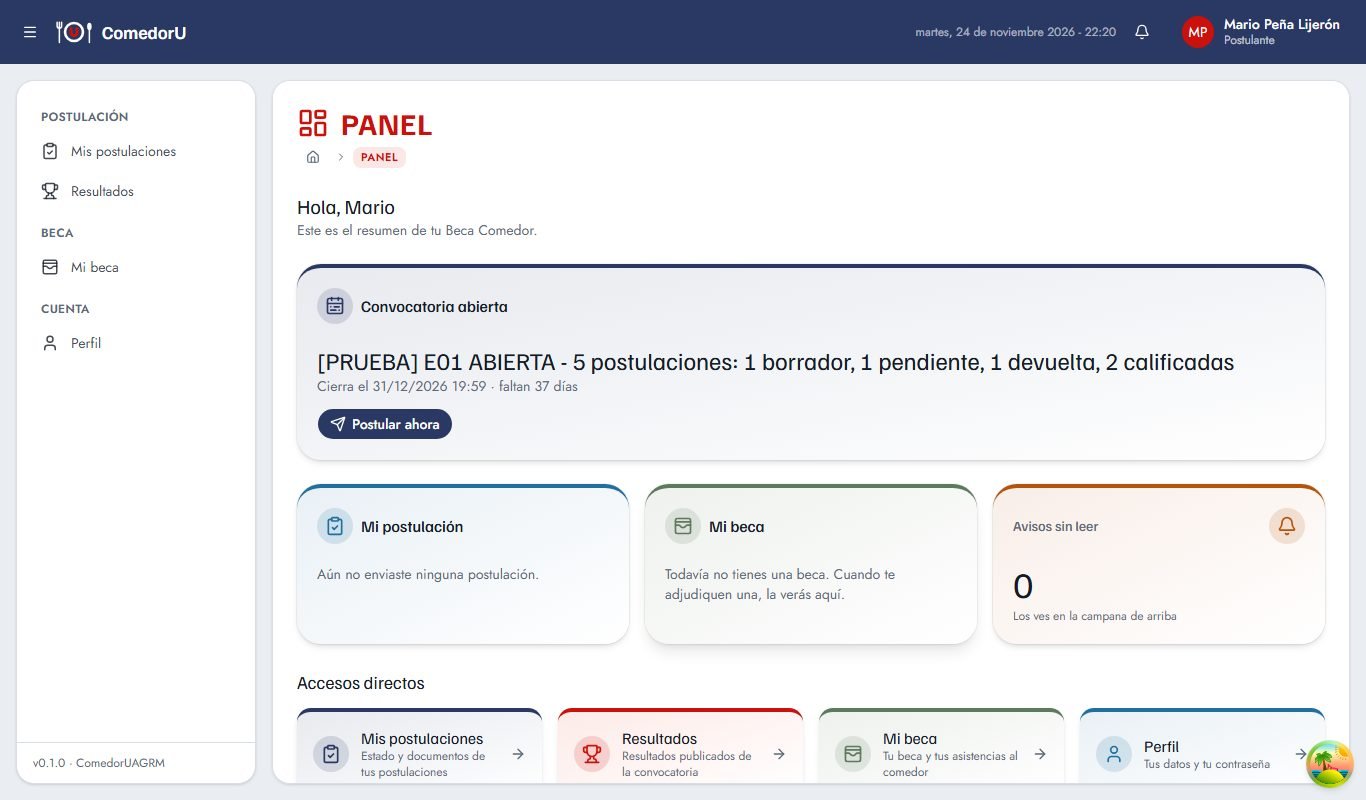
\includegraphics[width=0.93\linewidth,height=4.8cm,keepaspectratio]{images/210_CN_CU-15_A_login_nueva.jpg}}\vspace{2pt}\par\vspace{3pt}\fcolorbox{gray}{white}{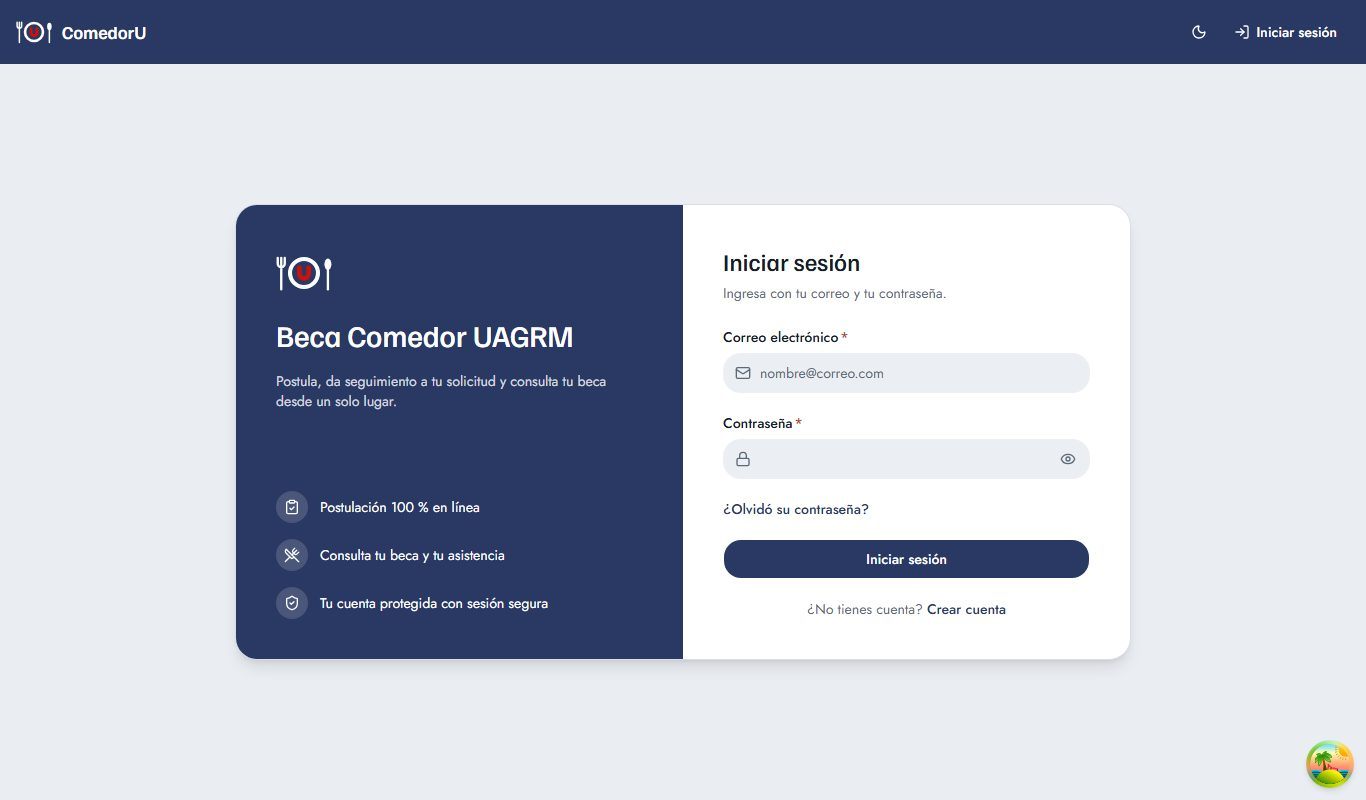
\includegraphics[width=0.93\linewidth,height=4.8cm,keepaspectratio]{images/211_CN_CU-15_A_final.jpg}}\vspace{2pt}\end{minipage}} \\
Resultado de prueba & {\textcolor{green!45!black}{\textbf{CORRECTO}}} \\
\end{longtable}
\endgroup
\addtocounter{table}{-1}
\vspace{-0.5\baselineskip}

\refstepcounter{table}\label{tab:cn_cu15_b}
\addcontentsline{lot}{table}{\protect\numberline{\thetable}CU-15. Recuperar contraseña y gestionar perfil (enlace de un solo uso)}
\noindent\textbf{Tabla~\thetable}\par\nopagebreak
\noindent\textit{CU-15. Recuperar contraseña y gestionar perfil (enlace de un solo uso)}\par\nopagebreak
\begingroup\footnotesize\linespread{1}\selectfont
\setlength{\LTleft}{0pt}\setlength{\LTright}{\fill}
\begin{longtable}{>{\raggedright\arraybackslash}p{3.6cm} >{\raggedright\arraybackslash}p{11.4cm}}
\toprule
\textbf{Campo} & \textbf{Contenido} \\
\midrule
\endfirsthead
\toprule
\textbf{Campo} & \textbf{Contenido} \\
\midrule
\endhead
\midrule
\multicolumn{2}{r}{\textit{Continúa en la siguiente página}} \\
\endfoot
\bottomrule
\multicolumn{2}{l}{\textit{Nota.} Elaboración propia a partir de la ejecución de la prueba.} \\
\endlastfoot
Nombre del caso de prueba & {CU-15. Recuperar contraseña y gestionar perfil (enlace de un solo uso)} \\
Descripción & {Un enlace ya usado no debe permitir cambiar la contraseña otra vez.} \\
Precondición & {El enlace del caso A ya fue usado.} \\
Datos de entrada & {El mismo enlace y la contraseña «OtraClave789».} \\
Condición de ejecución & {No aplica} \\
Captura de imagen inicial & {No aplica: la prueba comprueba un estado y no tiene pantalla previa distinta de la final.} \\
Pasos & {1. Abrir de nuevo el enlace del correo.\newline 2. Escribir una contraseña y su confirmación y pulsar «Guardar contraseña».} \\
Resultado esperado & {El sistema indica que el enlace ya no sirve.} \\
Resultado obtenido & {Se mostró «El enlace ya no sirve. Venció, ya se usó o pediste uno más reciente.» con la opción «Solicitar un enlace nuevo».} \\
Captura de imagen final & {\begin{minipage}[t]{\linewidth}\strut\par\vspace{3pt}\fcolorbox{gray}{white}{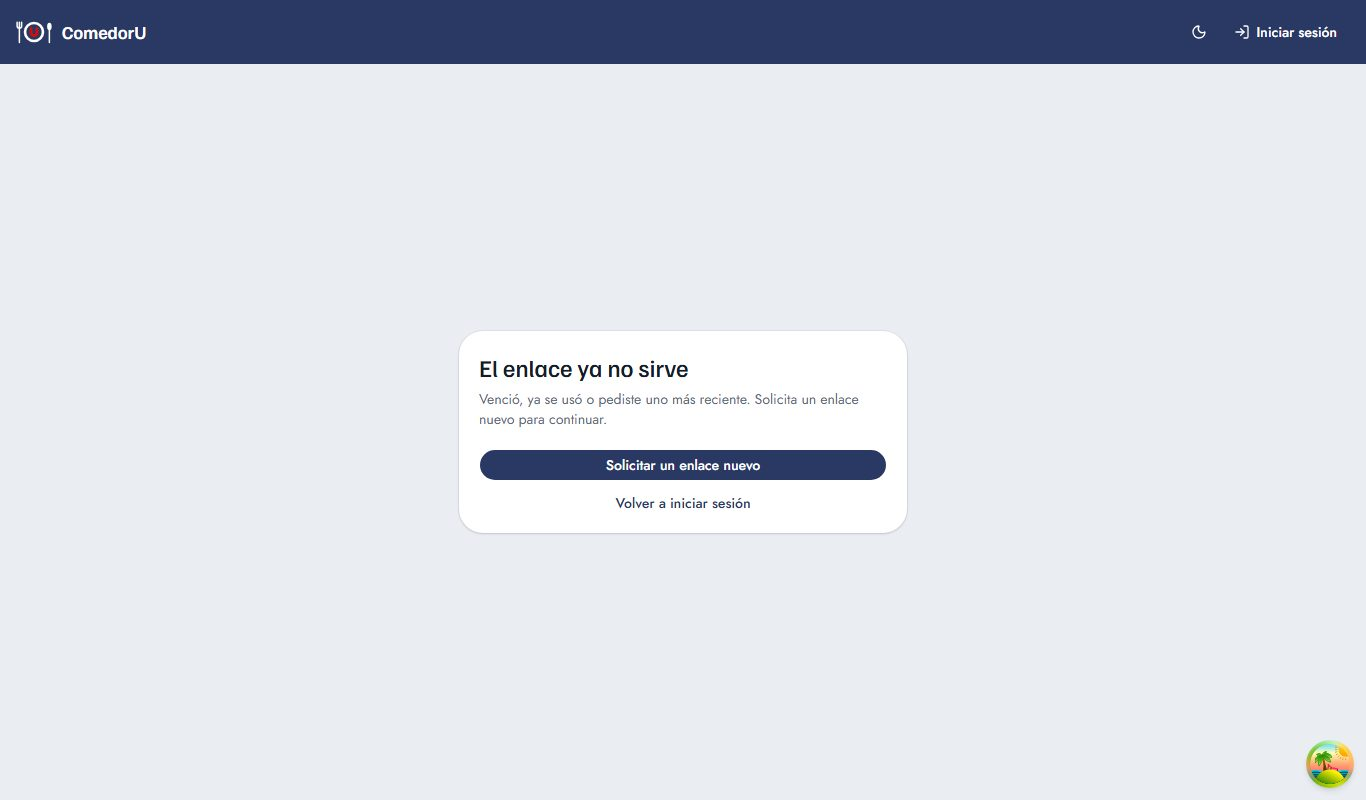
\includegraphics[width=0.93\linewidth,height=4.8cm,keepaspectratio]{images/212_CN_CU-15_B_enlace_reutilizado.jpg}}\vspace{2pt}\end{minipage}} \\
Resultado de prueba & {\textcolor{green!45!black}{\textbf{CORRECTO}}} \\
\end{longtable}
\endgroup
\addtocounter{table}{-1}
\vspace{-0.5\baselineskip}

\refstepcounter{table}\label{tab:cn_cu15_c}
\addcontentsline{lot}{table}{\protect\numberline{\thetable}CU-15. Recuperar contraseña y gestionar perfil (cambio desde el perfil)}
\noindent\textbf{Tabla~\thetable}\par\nopagebreak
\noindent\textit{CU-15. Recuperar contraseña y gestionar perfil (cambio desde el perfil)}\par\nopagebreak
\begingroup\footnotesize\linespread{1}\selectfont
\setlength{\LTleft}{0pt}\setlength{\LTright}{\fill}
\begin{longtable}{>{\raggedright\arraybackslash}p{3.6cm} >{\raggedright\arraybackslash}p{11.4cm}}
\toprule
\textbf{Campo} & \textbf{Contenido} \\
\midrule
\endfirsthead
\toprule
\textbf{Campo} & \textbf{Contenido} \\
\midrule
\endhead
\midrule
\multicolumn{2}{r}{\textit{Continúa en la siguiente página}} \\
\endfoot
\bottomrule
\multicolumn{2}{l}{\textit{Nota.} Elaboración propia a partir de la ejecución de la prueba.} \\
\endlastfoot
Nombre del caso de prueba & {CU-15. Recuperar contraseña y gestionar perfil (cambio desde el perfil)} \\
Descripción & {Desde \texttt{/\allowbreak{}perfil} el usuario cambia su contraseña confirmando la actual.} \\
Precondición & {Postulante con sesión abierta (contraseña actual «Clave123»).} \\
Datos de entrada & {Contraseña actual incorrecta «EstaNoEs1», luego la correcta «Clave123»; nueva «Nueva12345» y su confirmación.} \\
Condición de ejecución & {No aplica} \\
Captura de imagen inicial & {\begin{minipage}[t]{\linewidth}\strut\par\vspace{3pt}\fcolorbox{gray}{white}{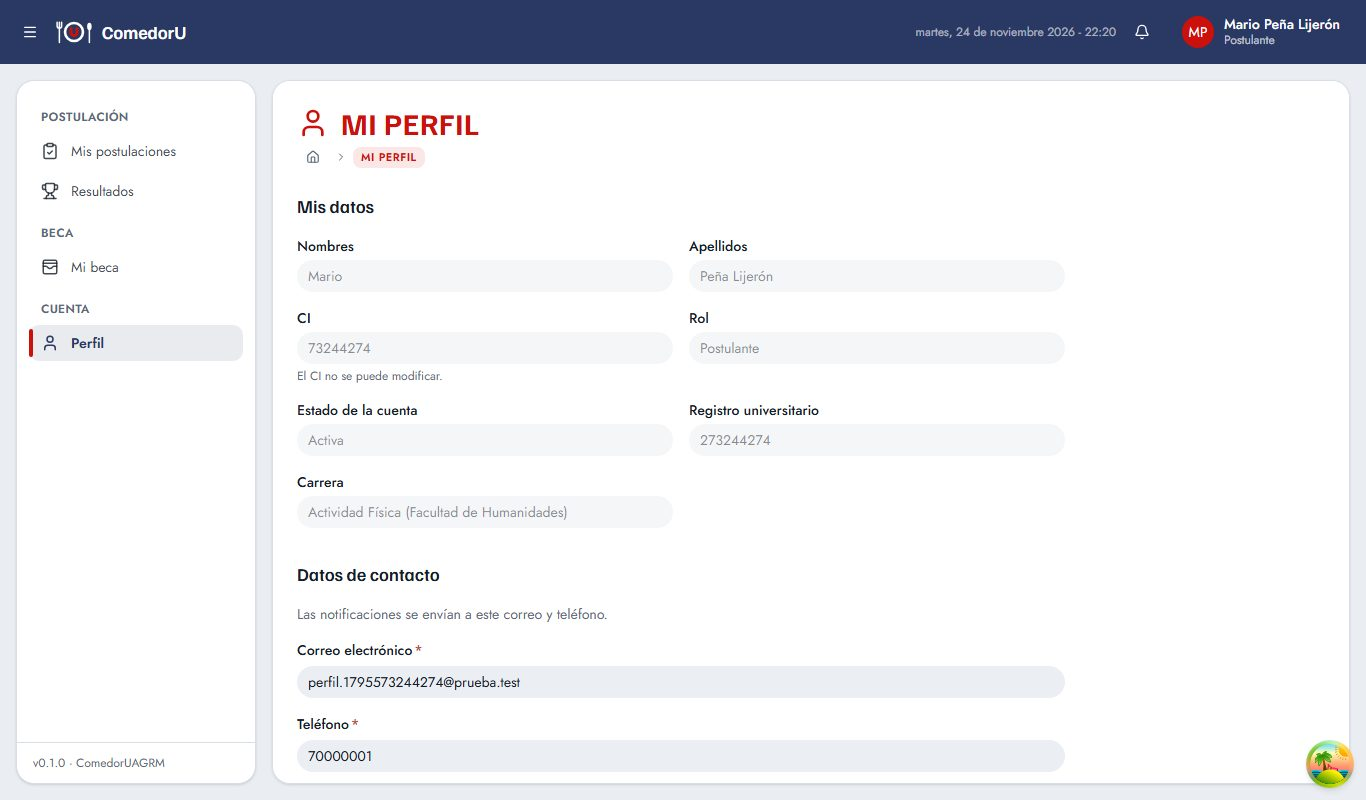
\includegraphics[width=0.93\linewidth,height=4.8cm,keepaspectratio]{images/213_CN_CU-15_C_inicial.jpg}}\vspace{2pt}\end{minipage}} \\
Pasos & {1. Abrir \texttt{/\allowbreak{}perfil}.\newline 2. Escribir una contraseña actual incorrecta, la nueva y su confirmación y pulsar «Cambiar contraseña».\newline 3. Corregir la contraseña actual y pulsar de nuevo «Cambiar contraseña».} \\
Resultado esperado & {Con la actual incorrecta se rechaza el cambio; con la correcta se actualiza y se avisa que las demás sesiones se cierran.} \\
Resultado obtenido & {Con la actual incorrecta apareció «La contraseña actual es incorrecta.» bajo el campo. Con la correcta apareció «Contraseña actualizada. Cerramos tu sesión en los demás dispositivos.».} \\
Captura de imagen final & {\begin{minipage}[t]{\linewidth}\strut\par\vspace{3pt}\fcolorbox{gray}{white}{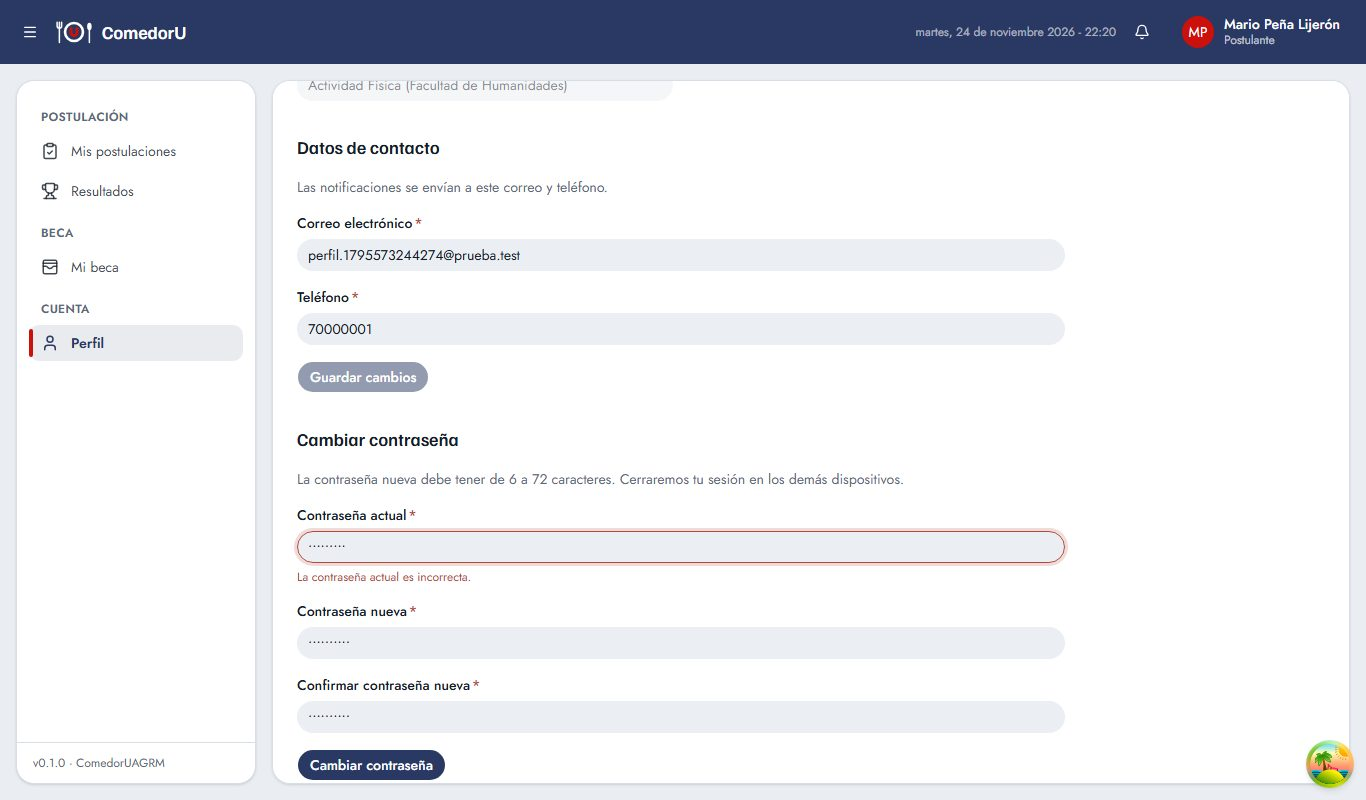
\includegraphics[width=0.93\linewidth,height=4.8cm,keepaspectratio]{images/214_CN_CU-15_C_final.jpg}}\vspace{2pt}\par\vspace{3pt}\fcolorbox{gray}{white}{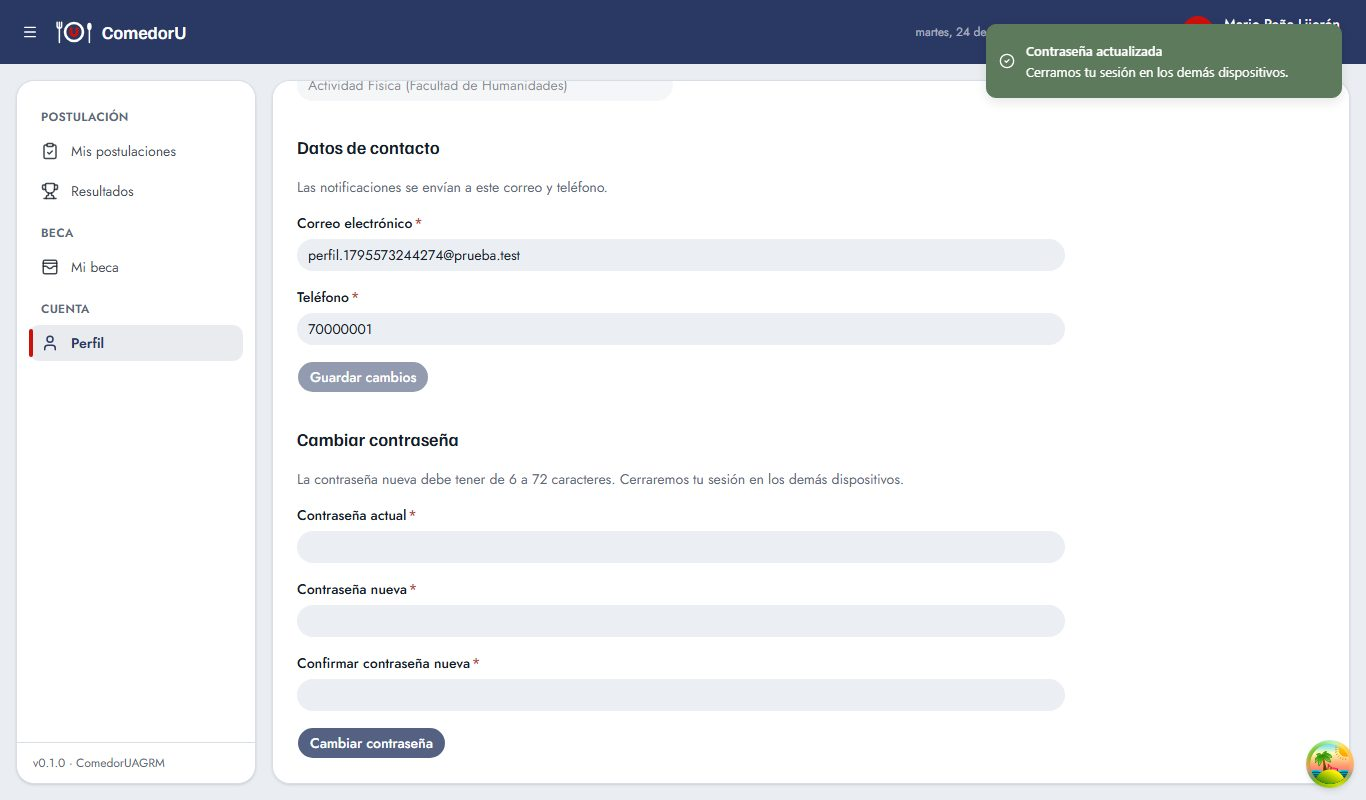
\includegraphics[width=0.93\linewidth,height=4.8cm,keepaspectratio]{images/215_CN_CU-15_C_cambio_correcto.jpg}}\vspace{2pt}\end{minipage}} \\
Resultado de prueba & {\textcolor{green!45!black}{\textbf{CORRECTO}}} \\
\end{longtable}
\endgroup
\addtocounter{table}{-1}
\vspace{-0.5\baselineskip}

\paragraph{CU-19. Devolver postulación para corrección.}\label{sec:cn_cu19} 

\refstepcounter{table}\label{tab:cn_cu19_a}
\addcontentsline{lot}{table}{\protect\numberline{\thetable}CU-19. Devolver postulación para corrección (devolución)}
\noindent\textbf{Tabla~\thetable}\par\nopagebreak
\noindent\textit{CU-19. Devolver postulación para corrección (devolución)}\par\nopagebreak
\begingroup\footnotesize\linespread{1}\selectfont
\setlength{\LTleft}{0pt}\setlength{\LTright}{\fill}
\begin{longtable}{>{\raggedright\arraybackslash}p{3.6cm} >{\raggedright\arraybackslash}p{11.4cm}}
\toprule
\textbf{Campo} & \textbf{Contenido} \\
\midrule
\endfirsthead
\toprule
\textbf{Campo} & \textbf{Contenido} \\
\midrule
\endhead
\midrule
\multicolumn{2}{r}{\textit{Continúa en la siguiente página}} \\
\endfoot
\bottomrule
\multicolumn{2}{l}{\textit{Nota.} Elaboración propia a partir de la ejecución de la prueba.} \\
\endlastfoot
Nombre del caso de prueba & {CU-19. Devolver postulación para corrección (devolución)} \\
Descripción & {El administrador devuelve al postulante una postulación calificada con auditoría, indicando el motivo.} \\
Precondición & {Sesión del administrador. Finalista 2 (Ana Zambrana Heredia) de «[PRUEBA] E04», calificada y con auditoría «Observado».} \\
Datos de entrada & {Motivo «Falta la fotocopia legible del certificado de ingresos; vuelva a presentarla.»} \\
Condición de ejecución & {El motivo es obligatorio (máximo 500 caracteres).} \\
Captura de imagen inicial & {\begin{minipage}[t]{\linewidth}\strut\par\vspace{3pt}\fcolorbox{gray}{white}{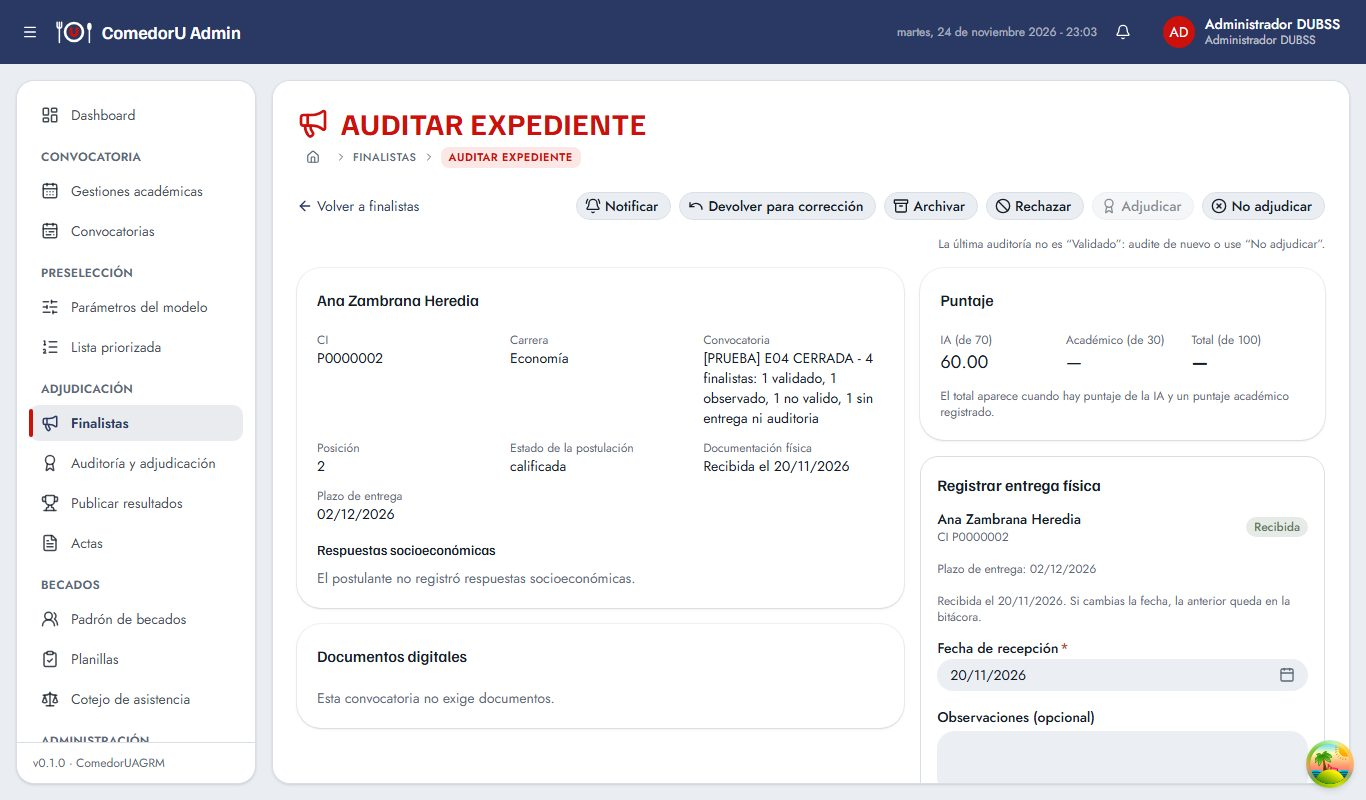
\includegraphics[width=0.93\linewidth,height=4.8cm,keepaspectratio]{images/216_CN_CU-19_A_inicial.jpg}}\vspace{2pt}\end{minipage}} \\
Pasos & {1. Abrir el expediente del finalista 2 de E04.\newline 2. Pulsar «Devolver para corrección».\newline 3. Escribir el motivo.\newline 4. Pulsar «Devolver».} \\
Resultado esperado & {El estado de la postulación pasa a «devuelta».} \\
Resultado obtenido & {La ventana indicó «Se avisará al postulante por la bandeja, el push y el correo». Tras confirmar, el expediente mostró «Estado de la postulación devuelta».} \\
Captura de imagen final & {\begin{minipage}[t]{\linewidth}\strut\par\vspace{3pt}\fcolorbox{gray}{white}{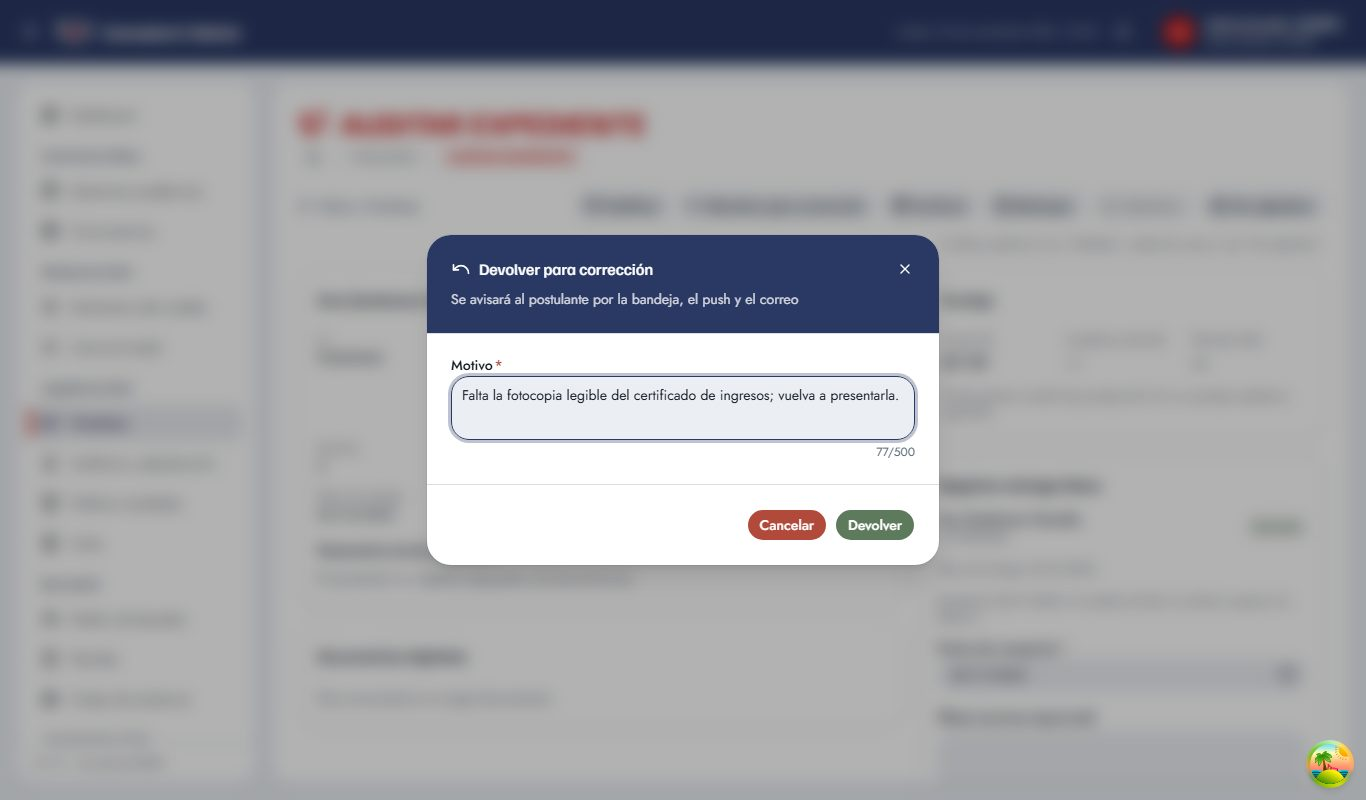
\includegraphics[width=0.93\linewidth,height=4.8cm,keepaspectratio]{images/217_CN_CU-19_A_motivo.jpg}}\vspace{2pt}\par\vspace{3pt}\fcolorbox{gray}{white}{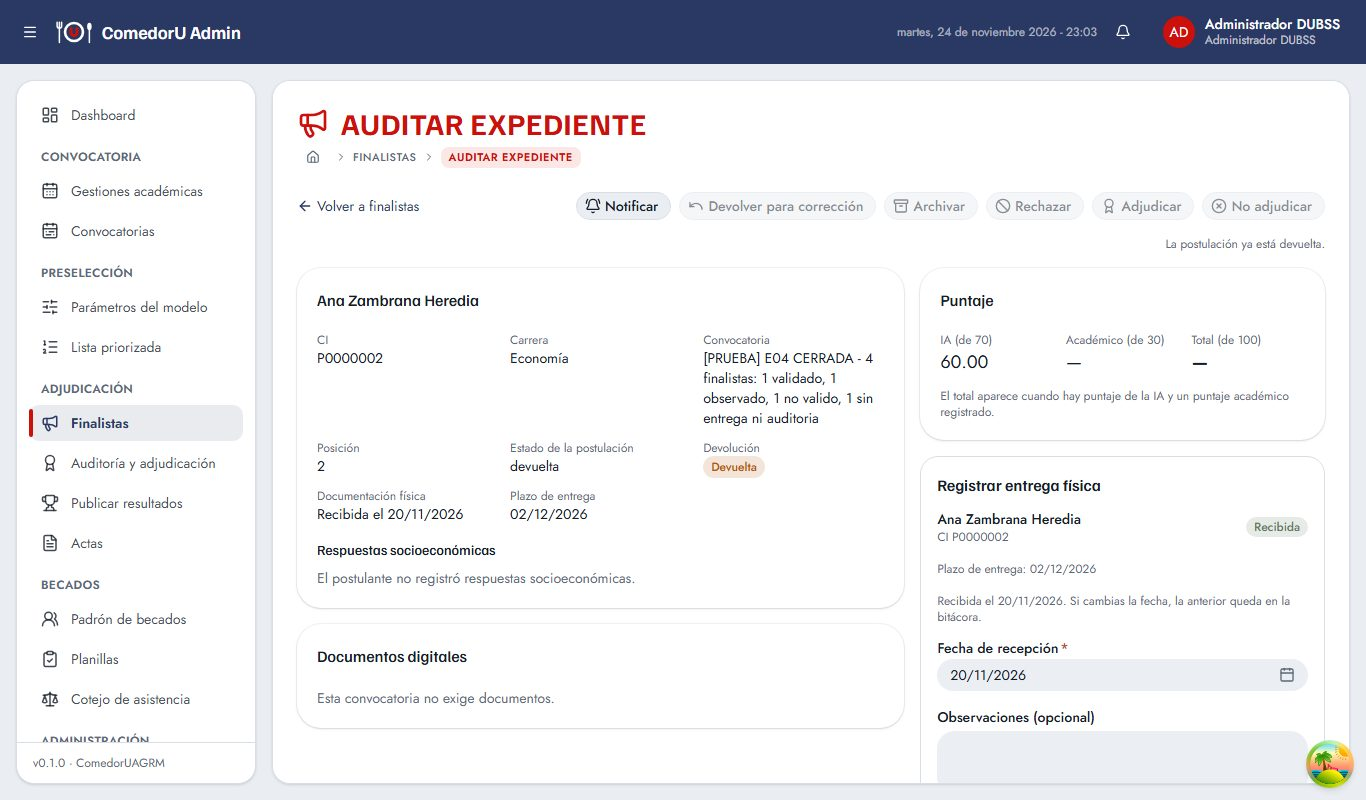
\includegraphics[width=0.93\linewidth,height=4.8cm,keepaspectratio]{images/218_CN_CU-19_A_final.jpg}}\vspace{2pt}\end{minipage}} \\
Resultado de prueba & {\textcolor{green!45!black}{\textbf{CORRECTO}}} \\
\end{longtable}
\endgroup
\addtocounter{table}{-1}
\vspace{-0.5\baselineskip}

\refstepcounter{table}\label{tab:cn_cu19_b}
\addcontentsline{lot}{table}{\protect\numberline{\thetable}CU-19. Devolver postulación para corrección (motivo vacío)}
\noindent\textbf{Tabla~\thetable}\par\nopagebreak
\noindent\textit{CU-19. Devolver postulación para corrección (motivo vacío)}\par\nopagebreak
\begingroup\footnotesize\linespread{1}\selectfont
\setlength{\LTleft}{0pt}\setlength{\LTright}{\fill}
\begin{longtable}{>{\raggedright\arraybackslash}p{3.6cm} >{\raggedright\arraybackslash}p{11.4cm}}
\toprule
\textbf{Campo} & \textbf{Contenido} \\
\midrule
\endfirsthead
\toprule
\textbf{Campo} & \textbf{Contenido} \\
\midrule
\endhead
\midrule
\multicolumn{2}{r}{\textit{Continúa en la siguiente página}} \\
\endfoot
\bottomrule
\multicolumn{2}{l}{\textit{Nota.} Elaboración propia a partir de la ejecución de la prueba.} \\
\endlastfoot
Nombre del caso de prueba & {CU-19. Devolver postulación para corrección (motivo vacío)} \\
Descripción & {El sistema exige el motivo de la devolución.} \\
Precondición & {Finalista 3 de E04 con auditoría.} \\
Datos de entrada & {Motivo vacío.} \\
Condición de ejecución & {No aplica} \\
Captura de imagen inicial & {\begin{minipage}[t]{\linewidth}\strut\par\vspace{3pt}\fcolorbox{gray}{white}{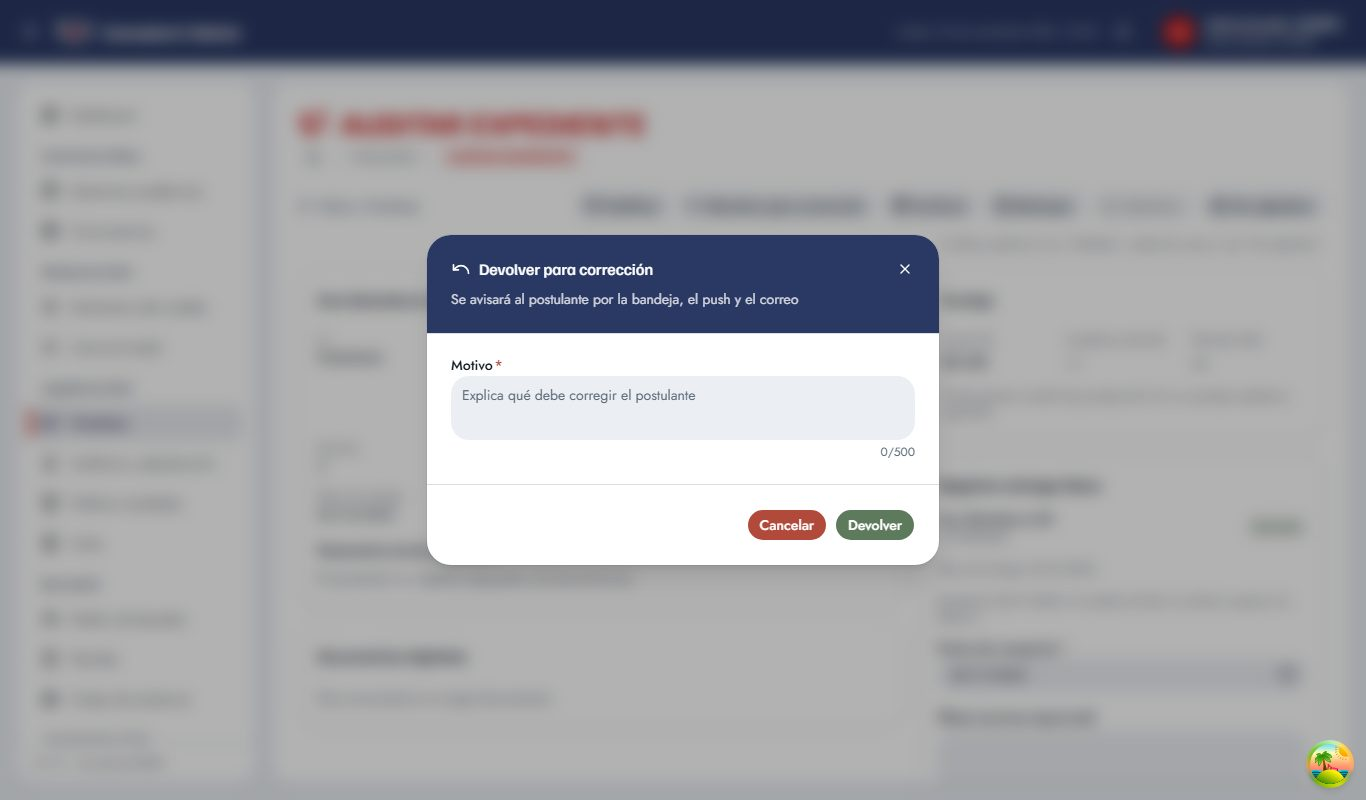
\includegraphics[width=0.93\linewidth,height=4.8cm,keepaspectratio]{images/219_CN_CU-19_B_inicial.jpg}}\vspace{2pt}\end{minipage}} \\
Pasos & {1. Abrir el expediente y pulsar «Devolver para corrección».\newline 2. Dejar vacío el motivo y pulsar «Devolver».} \\
Resultado esperado & {No se devuelve y se muestra que el motivo es obligatorio.} \\
Resultado obtenido & {La ventana siguió abierta con el mensaje «El motivo es obligatorio».} \\
Captura de imagen final & {\begin{minipage}[t]{\linewidth}\strut\par\vspace{3pt}\fcolorbox{gray}{white}{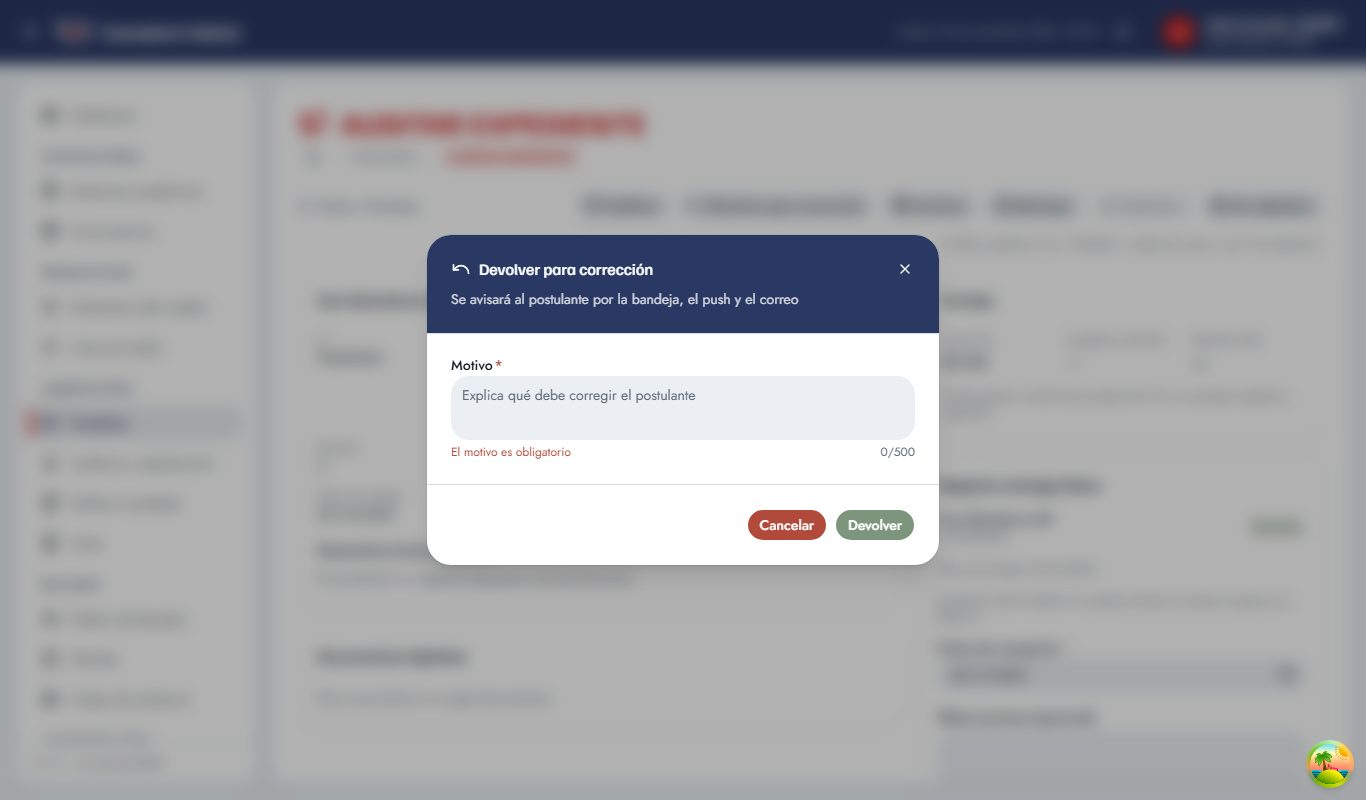
\includegraphics[width=0.93\linewidth,height=4.8cm,keepaspectratio]{images/220_CN_CU-19_B_final.jpg}}\vspace{2pt}\end{minipage}} \\
Resultado de prueba & {\textcolor{green!45!black}{\textbf{CORRECTO}}} \\
\end{longtable}
\endgroup
\addtocounter{table}{-1}
\vspace{-0.5\baselineskip}

\paragraph{CU-20. Archivar o rechazar postulación.}\label{sec:cn_cu20} 

\refstepcounter{table}\label{tab:cn_cu20_a}
\addcontentsline{lot}{table}{\protect\numberline{\thetable}CU-20. Archivar o rechazar postulación (archivar)}
\noindent\textbf{Tabla~\thetable}\par\nopagebreak
\noindent\textit{CU-20. Archivar o rechazar postulación (archivar)}\par\nopagebreak
\begingroup\footnotesize\linespread{1}\selectfont
\setlength{\LTleft}{0pt}\setlength{\LTright}{\fill}
\begin{longtable}{>{\raggedright\arraybackslash}p{3.6cm} >{\raggedright\arraybackslash}p{11.4cm}}
\toprule
\textbf{Campo} & \textbf{Contenido} \\
\midrule
\endfirsthead
\toprule
\textbf{Campo} & \textbf{Contenido} \\
\midrule
\endhead
\midrule
\multicolumn{2}{r}{\textit{Continúa en la siguiente página}} \\
\endfoot
\bottomrule
\multicolumn{2}{l}{\textit{Nota.} Elaboración propia a partir de la ejecución de la prueba.} \\
\endlastfoot
Nombre del caso de prueba & {CU-20. Archivar o rechazar postulación (archivar)} \\
Descripción & {El administrador archiva una postulación calificada indicando el motivo; la decisión es definitiva para la gestión.} \\
Precondición & {Finalista 3 (Ana Salvatierra Gil) de «[PRUEBA] E04», calificada, con resultados sin publicar.} \\
Datos de entrada & {Motivo «El postulante no cumple el requisito de matrícula vigente.»} \\
Condición de ejecución & {Motivo obligatorio (máximo 500); la convocatoria no debe tener resultados publicados.} \\
Captura de imagen inicial & {\begin{minipage}[t]{\linewidth}\strut\par\vspace{3pt}\fcolorbox{gray}{white}{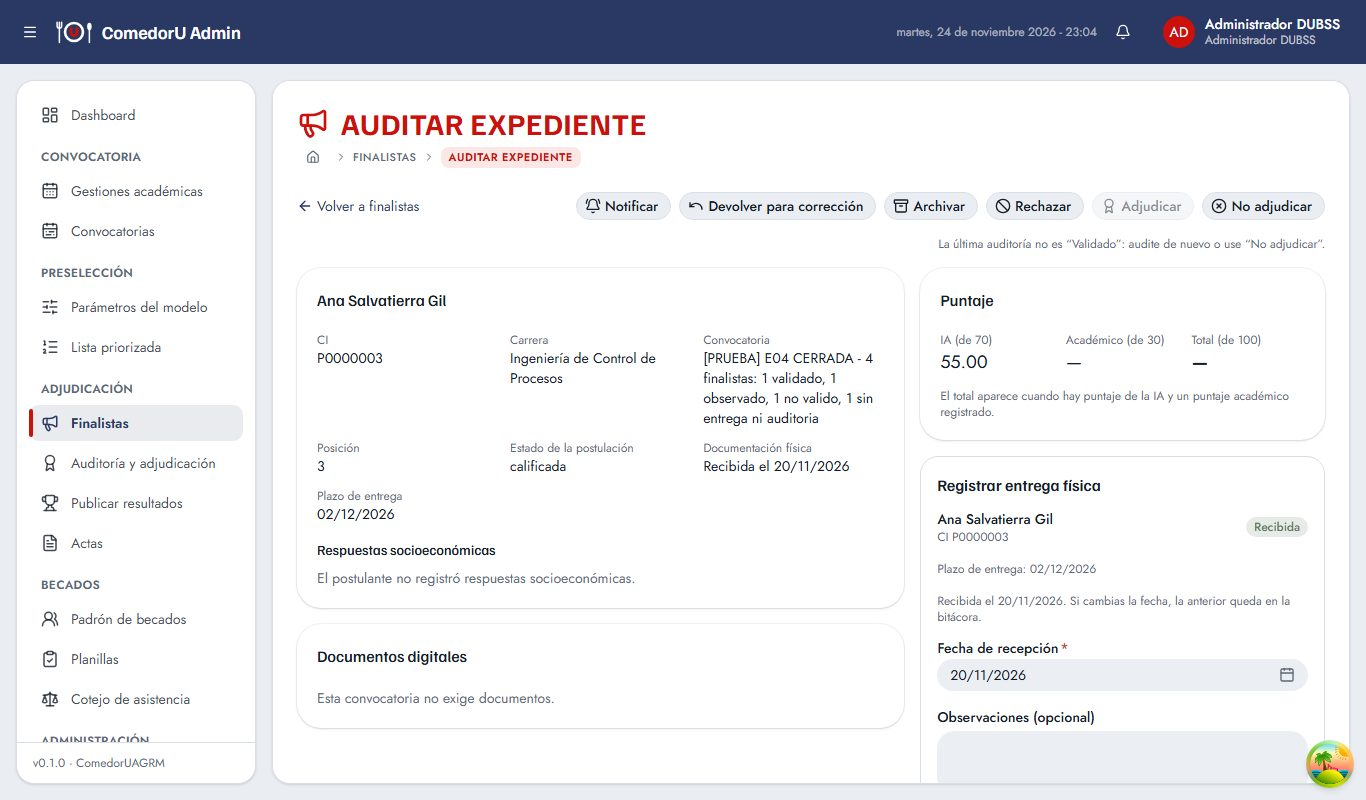
\includegraphics[width=0.93\linewidth,height=4.8cm,keepaspectratio]{images/221_CN_CU-20_A_inicial.jpg}}\vspace{2pt}\end{minipage}} \\
Pasos & {1. Abrir el expediente del finalista 3 de E04.\newline 2. Pulsar «Archivar».\newline 3. Escribir el motivo.\newline 4. Pulsar «Archivar» en la ventana.} \\
Resultado esperado & {La postulación queda «archivada».} \\
Resultado obtenido & {La ventana advirtió que la decisión es definitiva. Tras confirmar, el expediente mostró «Estado de la postulación archivada».} \\
Captura de imagen final & {\begin{minipage}[t]{\linewidth}\strut\par\vspace{3pt}\fcolorbox{gray}{white}{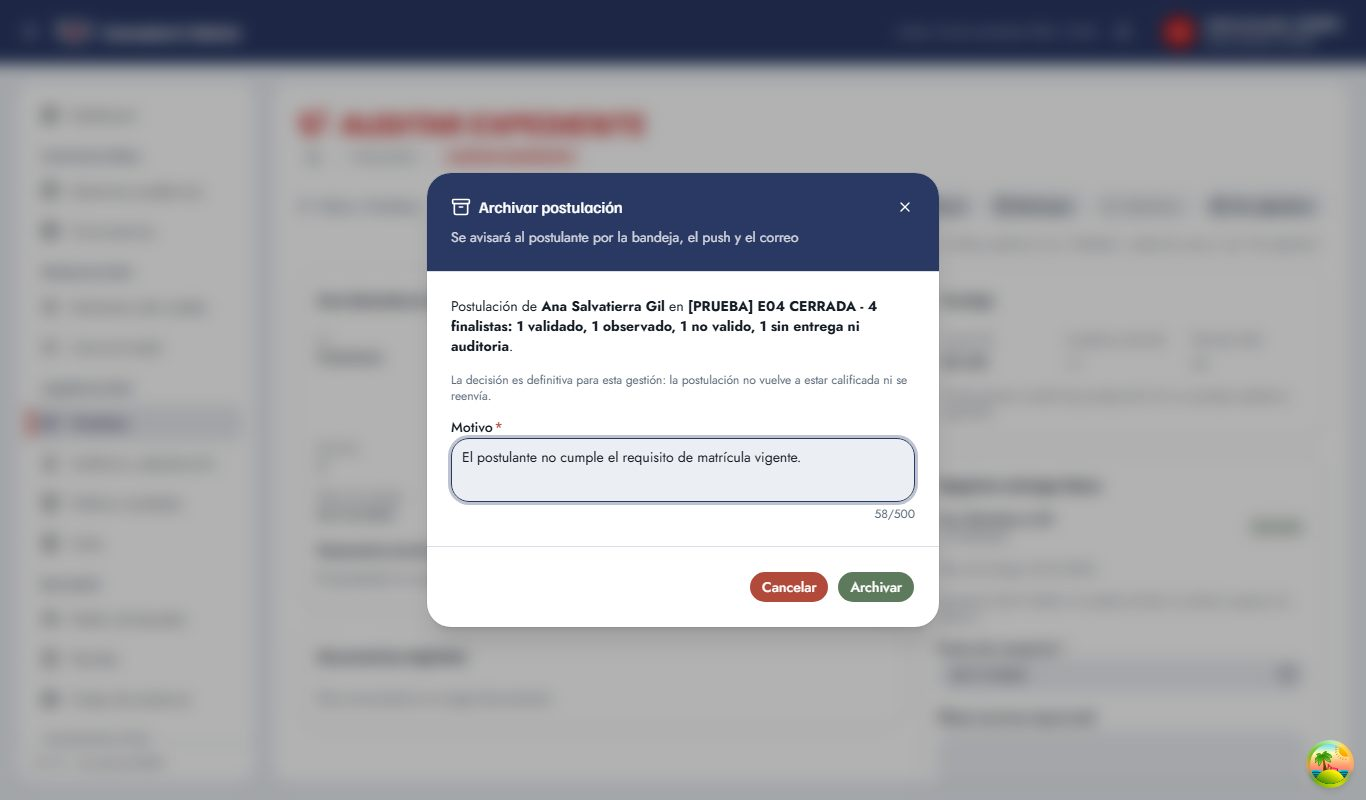
\includegraphics[width=0.93\linewidth,height=4.8cm,keepaspectratio]{images/222_CN_CU-20_A_motivo.jpg}}\vspace{2pt}\par\vspace{3pt}\fcolorbox{gray}{white}{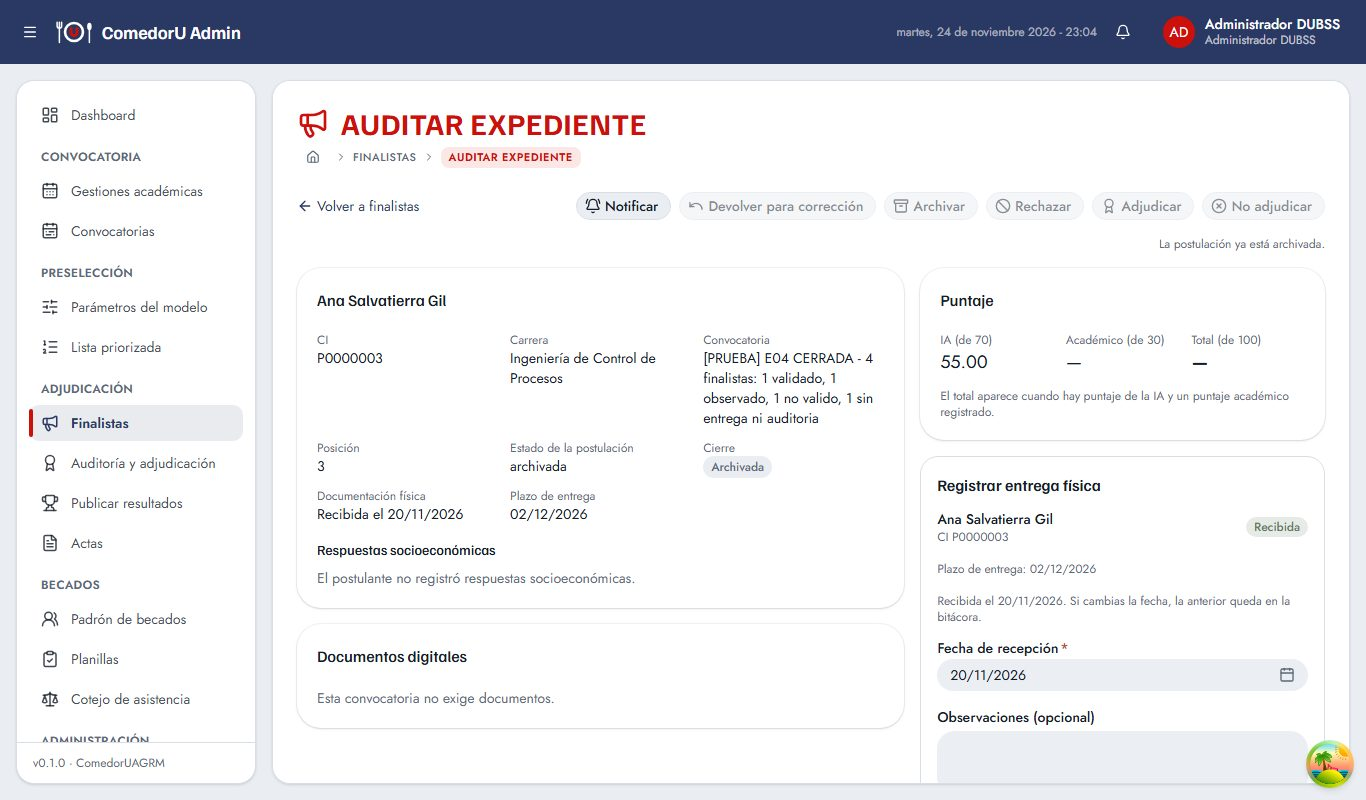
\includegraphics[width=0.93\linewidth,height=4.8cm,keepaspectratio]{images/223_CN_CU-20_A_final.jpg}}\vspace{2pt}\end{minipage}} \\
Resultado de prueba & {\textcolor{green!45!black}{\textbf{CORRECTO}}} \\
\end{longtable}
\endgroup
\addtocounter{table}{-1}
\vspace{-0.5\baselineskip}

\refstepcounter{table}\label{tab:cn_cu20_b}
\addcontentsline{lot}{table}{\protect\numberline{\thetable}CU-20. Archivar o rechazar postulación (motivo vacío)}
\noindent\textbf{Tabla~\thetable}\par\nopagebreak
\noindent\textit{CU-20. Archivar o rechazar postulación (motivo vacío)}\par\nopagebreak
\begingroup\footnotesize\linespread{1}\selectfont
\setlength{\LTleft}{0pt}\setlength{\LTright}{\fill}
\begin{longtable}{>{\raggedright\arraybackslash}p{3.6cm} >{\raggedright\arraybackslash}p{11.4cm}}
\toprule
\textbf{Campo} & \textbf{Contenido} \\
\midrule
\endfirsthead
\toprule
\textbf{Campo} & \textbf{Contenido} \\
\midrule
\endhead
\midrule
\multicolumn{2}{r}{\textit{Continúa en la siguiente página}} \\
\endfoot
\bottomrule
\multicolumn{2}{l}{\textit{Nota.} Elaboración propia a partir de la ejecución de la prueba.} \\
\endlastfoot
Nombre del caso de prueba & {CU-20. Archivar o rechazar postulación (motivo vacío)} \\
Descripción & {El sistema exige el motivo.} \\
Precondición & {Finalista 4 (Mario Cuéllar Soliz) de E04.} \\
Datos de entrada & {Motivo vacío.} \\
Condición de ejecución & {No aplica} \\
Captura de imagen inicial & {\begin{minipage}[t]{\linewidth}\strut\par\vspace{3pt}\fcolorbox{gray}{white}{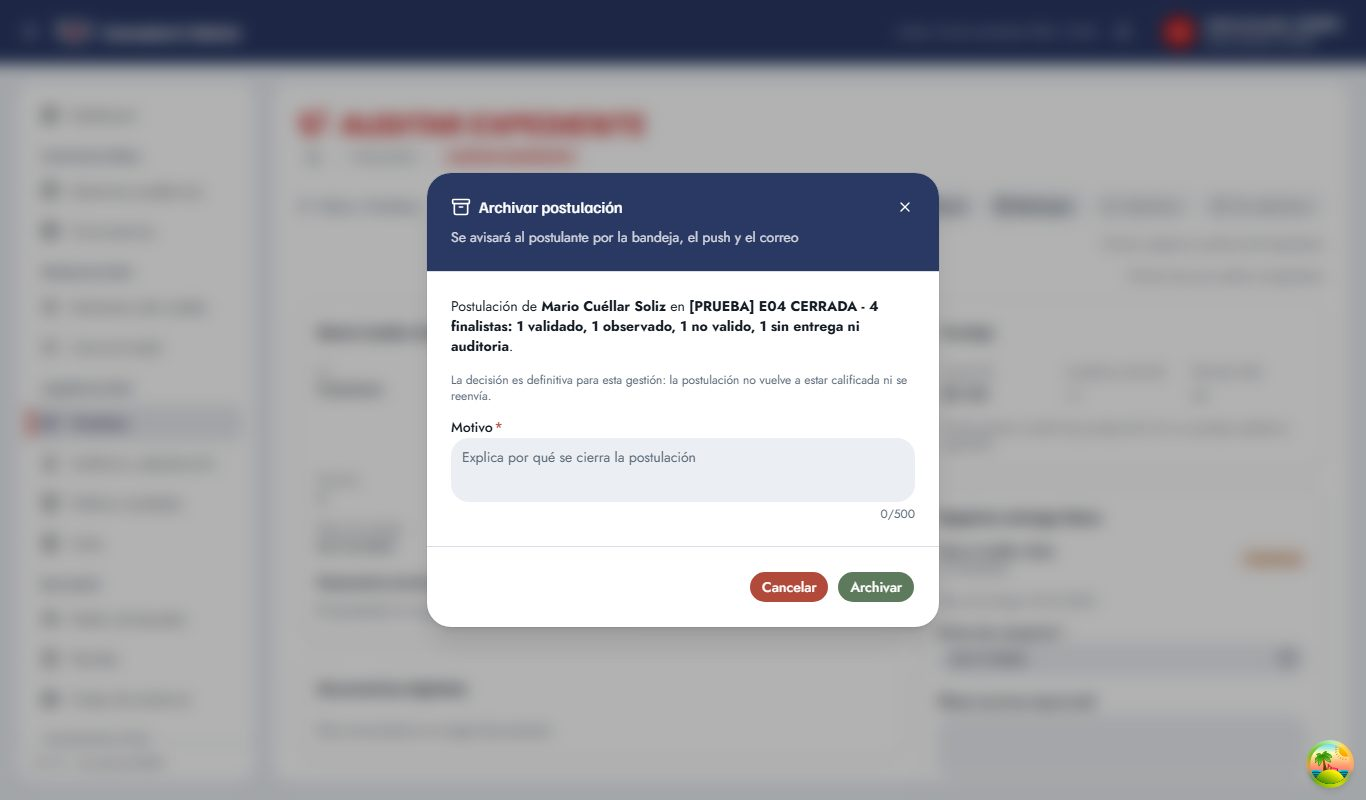
\includegraphics[width=0.93\linewidth,height=4.8cm,keepaspectratio]{images/224_CN_CU-20_B_inicial.jpg}}\vspace{2pt}\end{minipage}} \\
Pasos & {1. Abrir el expediente y pulsar «Archivar».\newline 2. Pulsar «Archivar» sin escribir el motivo.} \\
Resultado esperado & {No se archiva y se muestra que el motivo es obligatorio.} \\
Resultado obtenido & {La ventana siguió abierta con «El motivo es obligatorio».} \\
Captura de imagen final & {\begin{minipage}[t]{\linewidth}\strut\par\vspace{3pt}\fcolorbox{gray}{white}{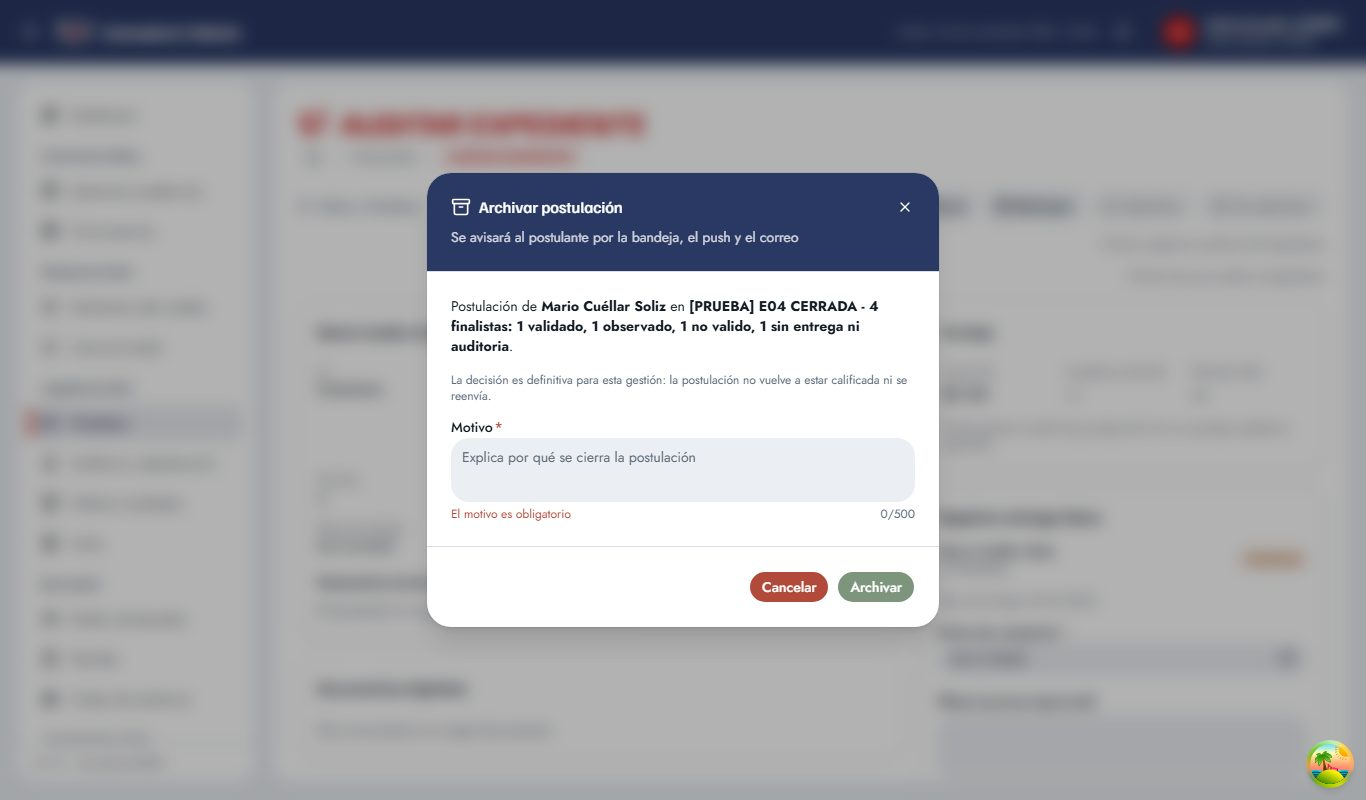
\includegraphics[width=0.93\linewidth,height=4.8cm,keepaspectratio]{images/225_CN_CU-20_B_final.jpg}}\vspace{2pt}\end{minipage}} \\
Resultado de prueba & {\textcolor{green!45!black}{\textbf{CORRECTO}}} \\
\end{longtable}
\endgroup
\addtocounter{table}{-1}
\vspace{-0.5\baselineskip}

\paragraph{CU-21. Notificar finalistas y publicar comunicados.}\label{sec:cn_cu21} 

\refstepcounter{table}\label{tab:cn_cu21_a}
\addcontentsline{lot}{table}{\protect\numberline{\thetable}CU-21. Notificar finalistas y publicar comunicados (notificación)}
\noindent\textbf{Tabla~\thetable}\par\nopagebreak
\noindent\textit{CU-21. Notificar finalistas y publicar comunicados (notificación)}\par\nopagebreak
\begingroup\footnotesize\linespread{1}\selectfont
\setlength{\LTleft}{0pt}\setlength{\LTright}{\fill}
\begin{longtable}{>{\raggedright\arraybackslash}p{3.6cm} >{\raggedright\arraybackslash}p{11.4cm}}
\toprule
\textbf{Campo} & \textbf{Contenido} \\
\midrule
\endfirsthead
\toprule
\textbf{Campo} & \textbf{Contenido} \\
\midrule
\endhead
\midrule
\multicolumn{2}{r}{\textit{Continúa en la siguiente página}} \\
\endfoot
\bottomrule
\multicolumn{2}{l}{\textit{Nota.} Elaboración propia a partir de la ejecución de la prueba.} \\
\endlastfoot
Nombre del caso de prueba & {CU-21. Notificar finalistas y publicar comunicados (notificación)} \\
Descripción & {El administrador avisa a un finalista el plazo, lugar y documentos de entrega; el aviso llega por bandeja, push y correo.} \\
Precondición & {Sesión del administrador. Convocatoria sembrada «[PRUEBA] E03» con 4 finalistas sin notificar.} \\
Datos de entrada & {Finalista 1 (Elena Suárez Molina), plazo 15/12/2026, lugar y horario «Oficina de la DUBSS, planta baja, de 08:00 a 12:00», documentos «Fotocopia de carnet, certificado de ingresos y boleta de luz».} \\
Condición de ejecución & {El plazo debe ser posterior a la fecha de hoy.} \\
Captura de imagen inicial & {\begin{minipage}[t]{\linewidth}\strut\par\vspace{3pt}\fcolorbox{gray}{white}{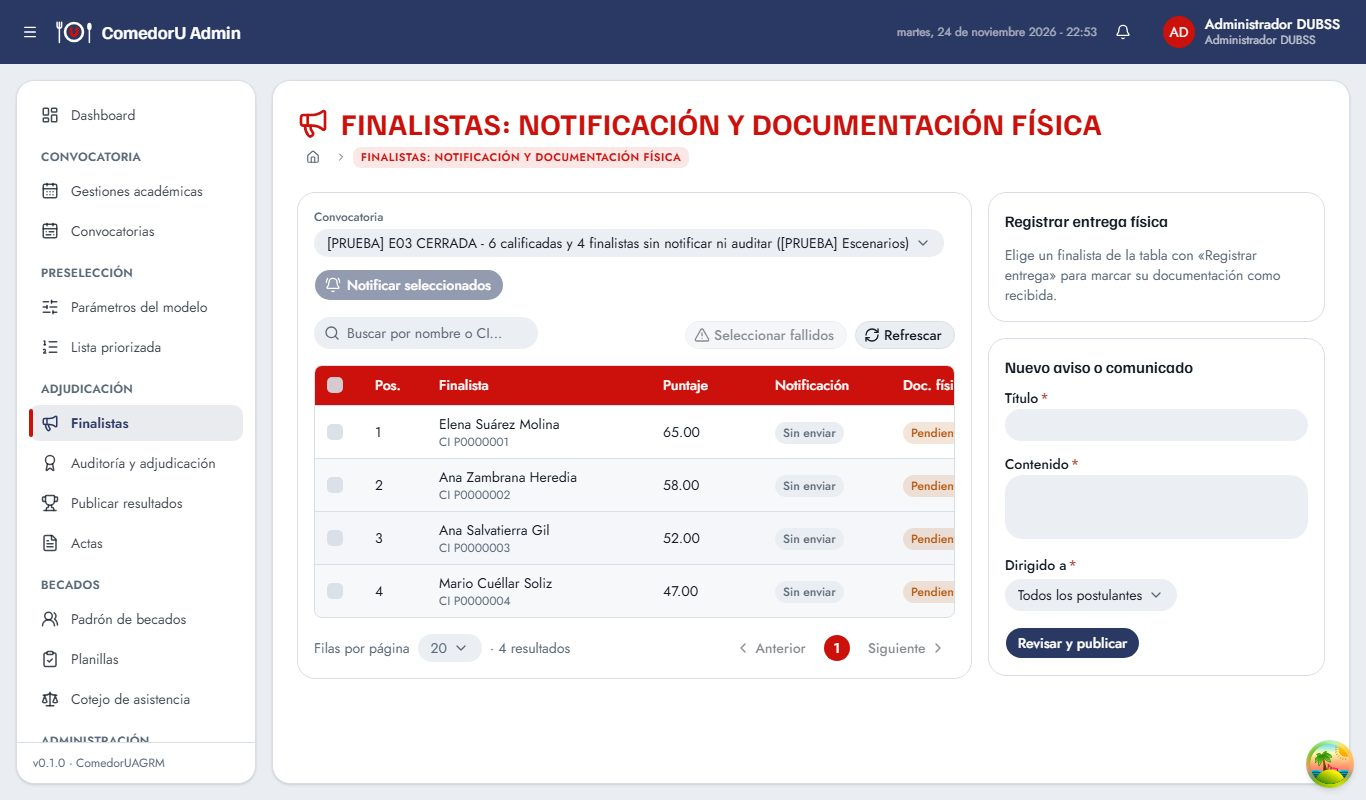
\includegraphics[width=0.93\linewidth,height=4.8cm,keepaspectratio]{images/226_CN_CU-21_A_inicial.jpg}}\vspace{2pt}\end{minipage}} \\
Pasos & {1. Abrir «Finalistas» y elegir la convocatoria E03.\newline 2. Marcar a Elena y pulsar «Notificar seleccionados».\newline 3. Elegir el plazo en el calendario y completar lugar y documentos; pulsar «Enviar aviso».\newline 4. Pulsar «Confirmar envío» en la ventana de confirmación.} \\
Resultado esperado & {El sistema informa el envío, el finalista pasa a «Enviada» y el correo llega a su bandeja.} \\
Resultado obtenido & {La ventana «Resultado del envío» dijo «Se está enviando el aviso a 1 finalista». En la tabla Elena quedó en «Enviada» y Mailpit recibió «Entrega de documentación física - Beca Comedor» para \texttt{postulante.\allowbreak{}0000001@\allowbreak{}prueba.\allowbreak{}local}.} \\
Captura de imagen final & {\begin{minipage}[t]{\linewidth}\strut\par\vspace{3pt}\fcolorbox{gray}{white}{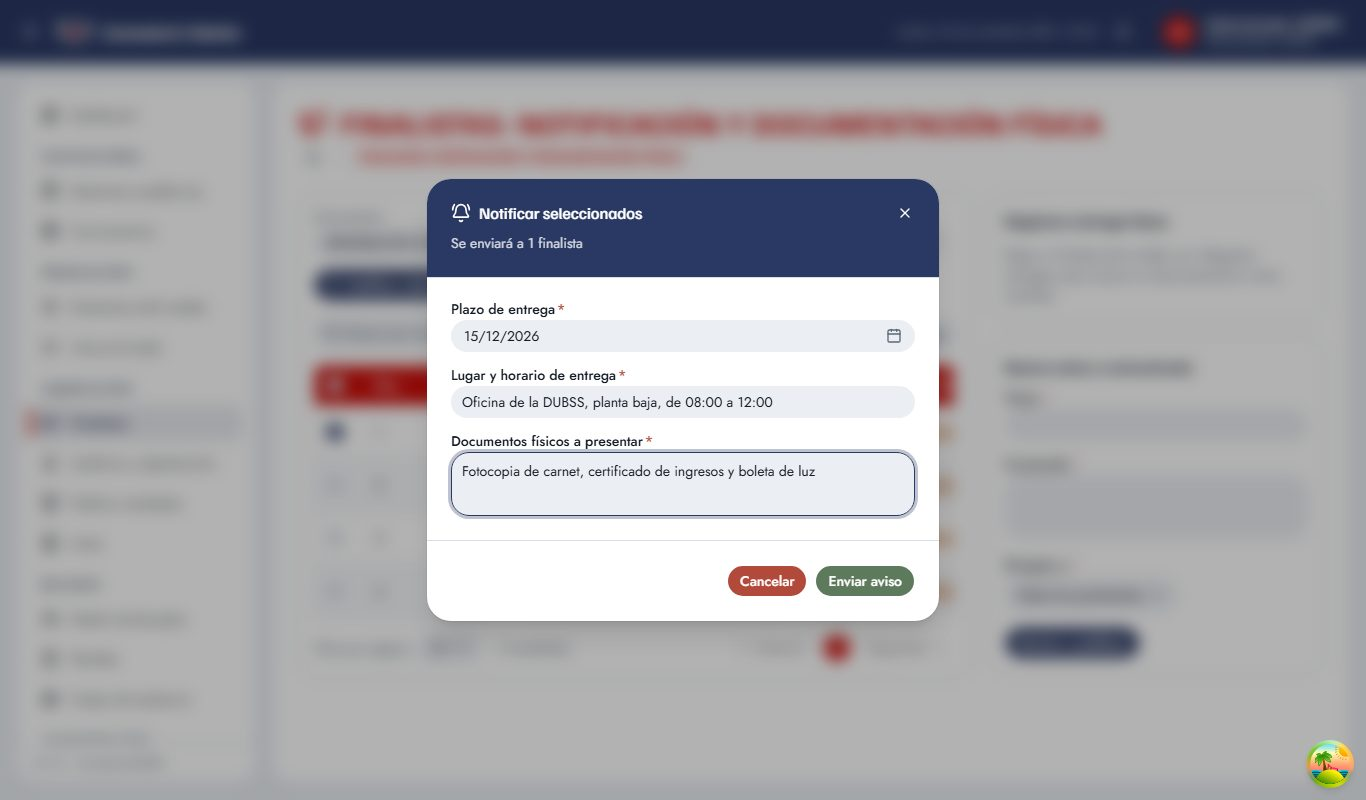
\includegraphics[width=0.93\linewidth,height=4.8cm,keepaspectratio]{images/227_CN_CU-21_A_formulario.jpg}}\vspace{2pt}\par\vspace{3pt}\fcolorbox{gray}{white}{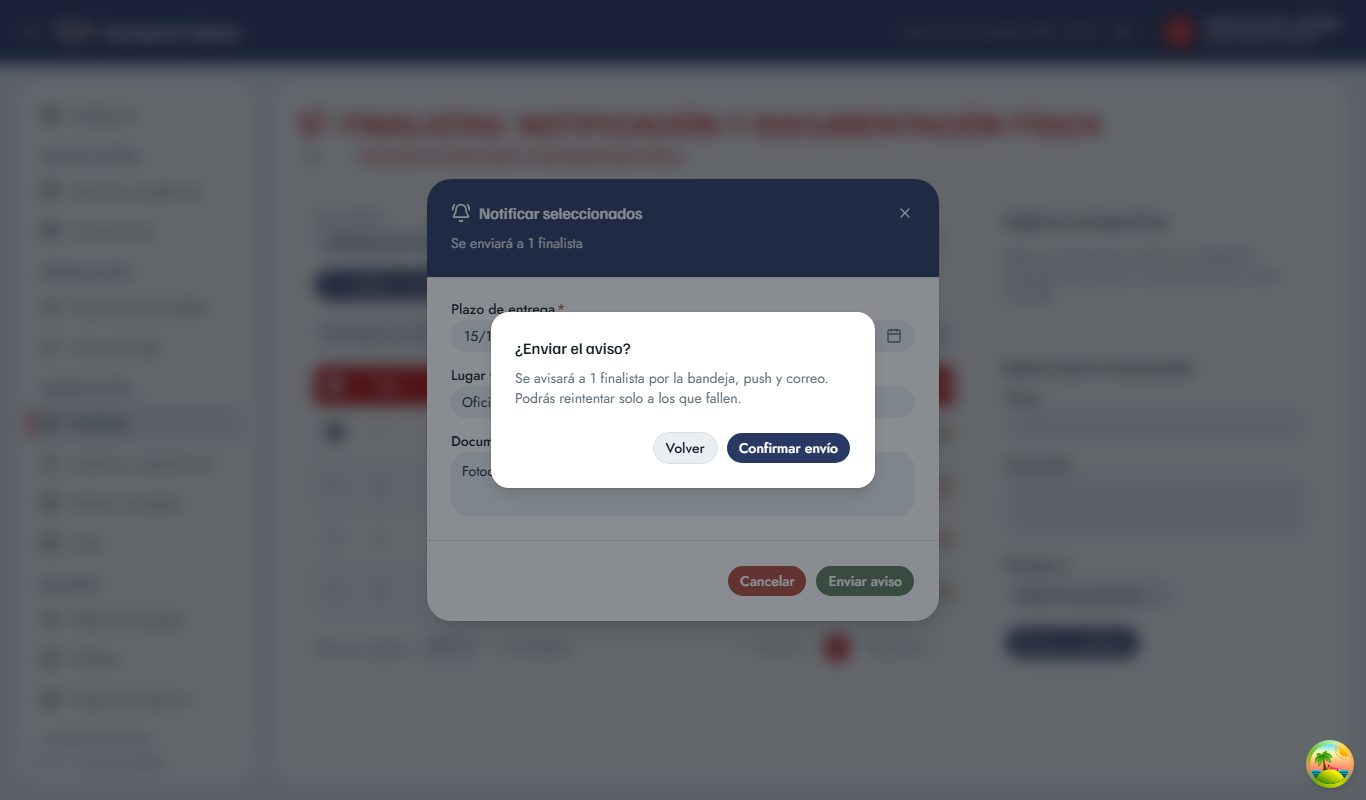
\includegraphics[width=0.93\linewidth,height=4.8cm,keepaspectratio]{images/228_CN_CU-21_A_confirmacion.jpg}}\vspace{2pt}\par\vspace{3pt}\fcolorbox{gray}{white}{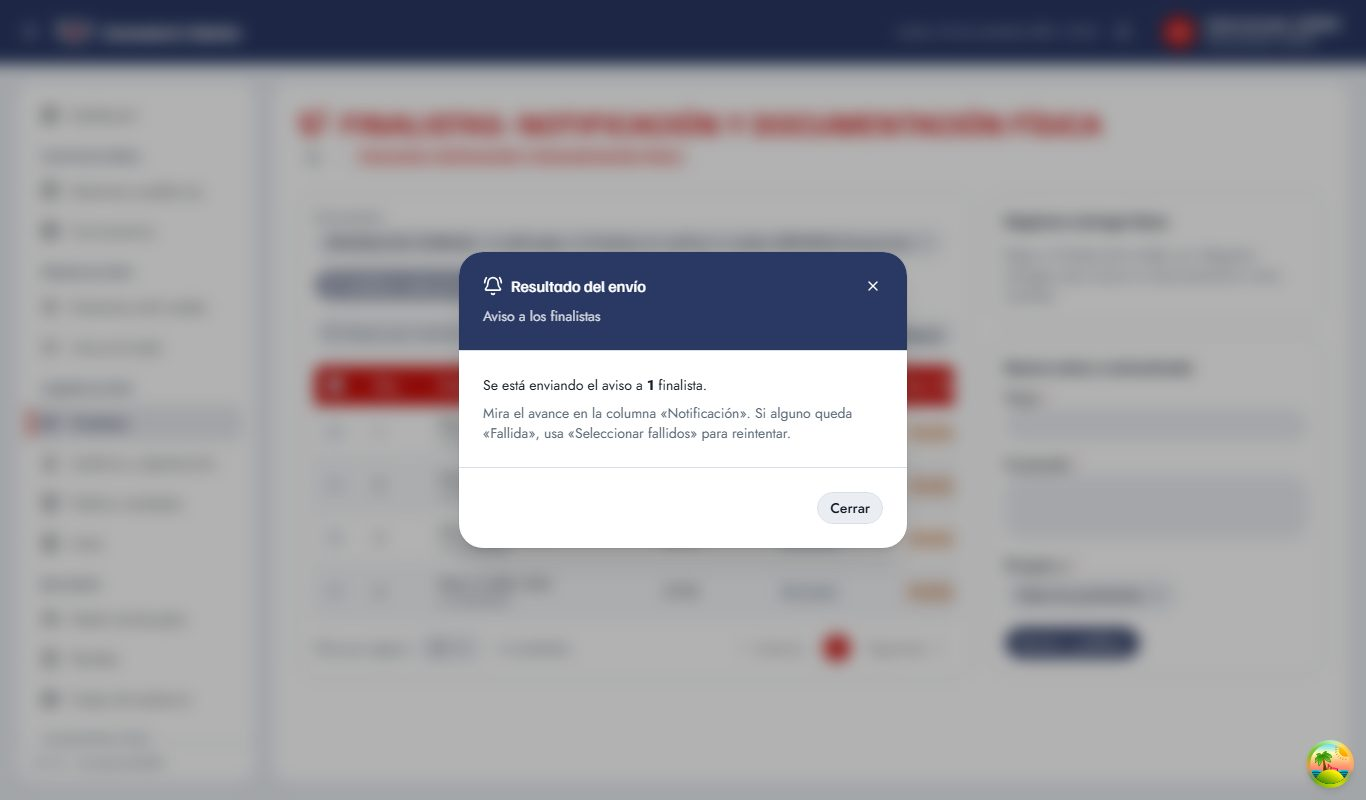
\includegraphics[width=0.93\linewidth,height=4.8cm,keepaspectratio]{images/229_CN_CU-21_A_final.jpg}}\vspace{2pt}\par\vspace{3pt}\fcolorbox{gray}{white}{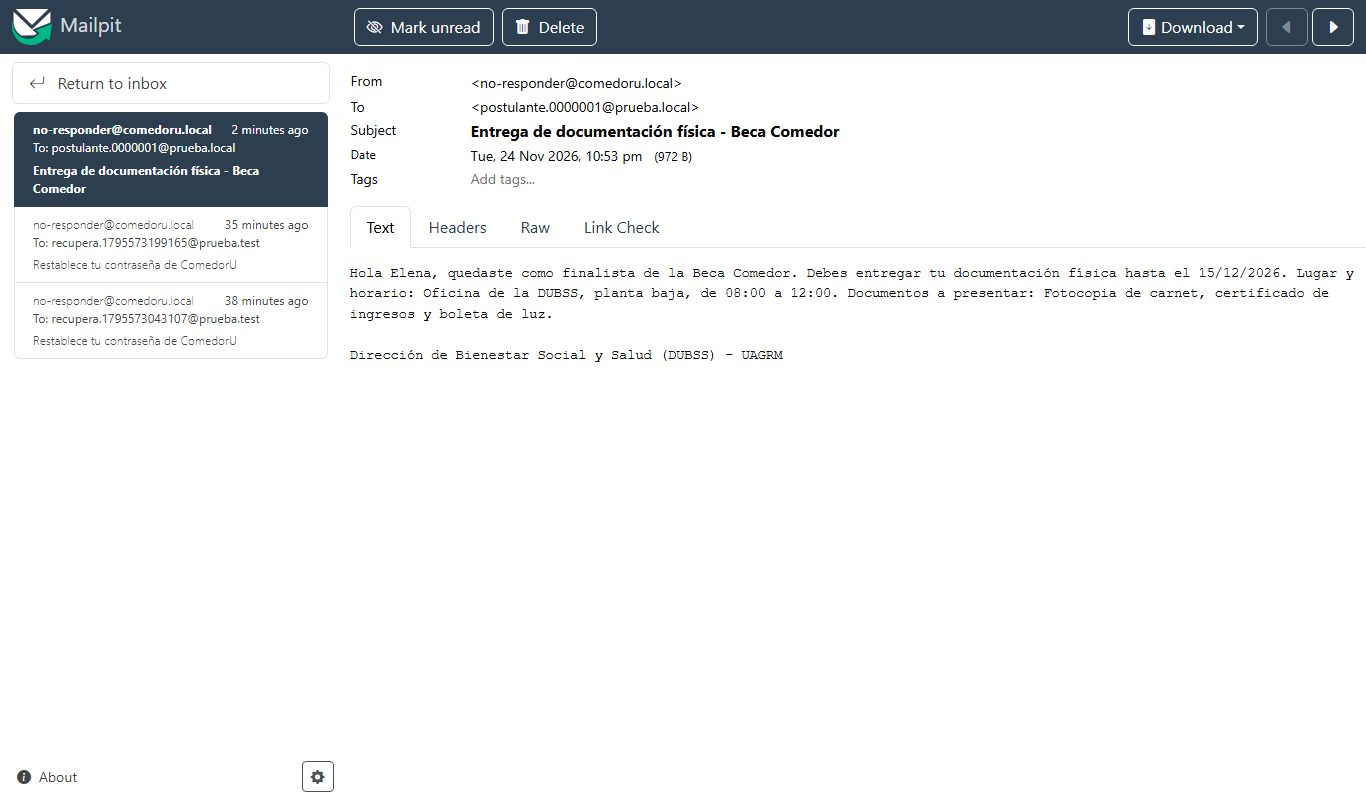
\includegraphics[width=0.93\linewidth,height=4.8cm,keepaspectratio]{images/230_CN_CU-21_A_correo_mailpit.jpg}}\vspace{2pt}\par\vspace{3pt}\fcolorbox{gray}{white}{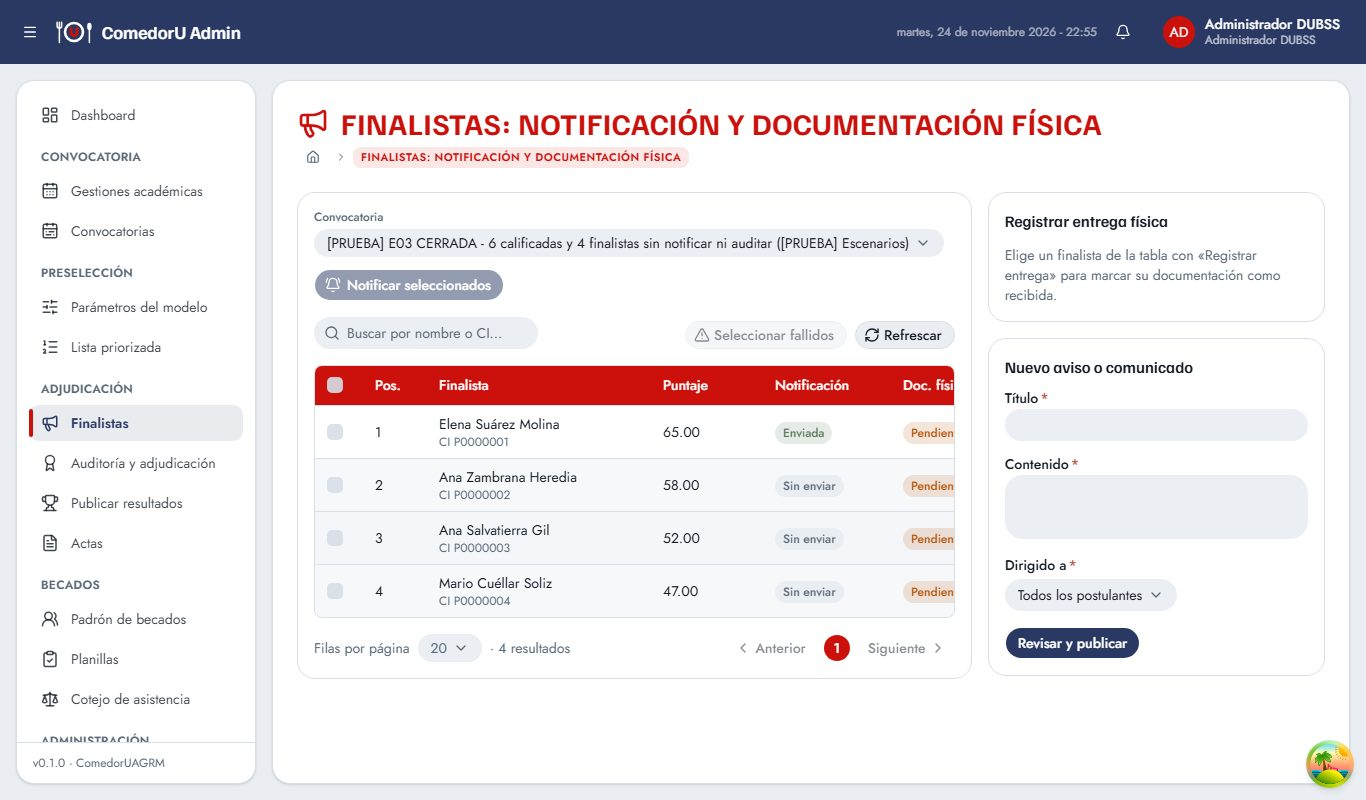
\includegraphics[width=0.93\linewidth,height=4.8cm,keepaspectratio]{images/231_CN_CU-21_A_final_tabla.jpg}}\vspace{2pt}\end{minipage}} \\
Resultado de prueba & {\textcolor{green!45!black}{\textbf{CORRECTO}}} \\
\end{longtable}
\endgroup
\addtocounter{table}{-1}
\vspace{-0.5\baselineskip}

\refstepcounter{table}\label{tab:cn_cu21_b}
\addcontentsline{lot}{table}{\protect\numberline{\thetable}CU-21. Notificar finalistas y publicar comunicados (plazo inválido)}
\noindent\textbf{Tabla~\thetable}\par\nopagebreak
\noindent\textit{CU-21. Notificar finalistas y publicar comunicados (plazo inválido)}\par\nopagebreak
\begingroup\footnotesize\linespread{1}\selectfont
\setlength{\LTleft}{0pt}\setlength{\LTright}{\fill}
\begin{longtable}{>{\raggedright\arraybackslash}p{3.6cm} >{\raggedright\arraybackslash}p{11.4cm}}
\toprule
\textbf{Campo} & \textbf{Contenido} \\
\midrule
\endfirsthead
\toprule
\textbf{Campo} & \textbf{Contenido} \\
\midrule
\endhead
\midrule
\multicolumn{2}{r}{\textit{Continúa en la siguiente página}} \\
\endfoot
\bottomrule
\multicolumn{2}{l}{\textit{Nota.} Elaboración propia a partir de la ejecución de la prueba.} \\
\endlastfoot
Nombre del caso de prueba & {CU-21. Notificar finalistas y publicar comunicados (plazo inválido)} \\
Descripción & {El sistema no deja enviar el aviso con un plazo vencido o vacío.} \\
Precondición & {Finalista 2 (Ana Zambrana Heredia) de E03 sin notificar.} \\
Datos de entrada & {Intento de elegir el 1/11/2026 (fecha pasada); lugar «Oficina de la DUBSS»; documentos «Carnet».} \\
Condición de ejecución & {No aplica} \\
Captura de imagen inicial & {\begin{minipage}[t]{\linewidth}\strut\par\vspace{3pt}\fcolorbox{gray}{white}{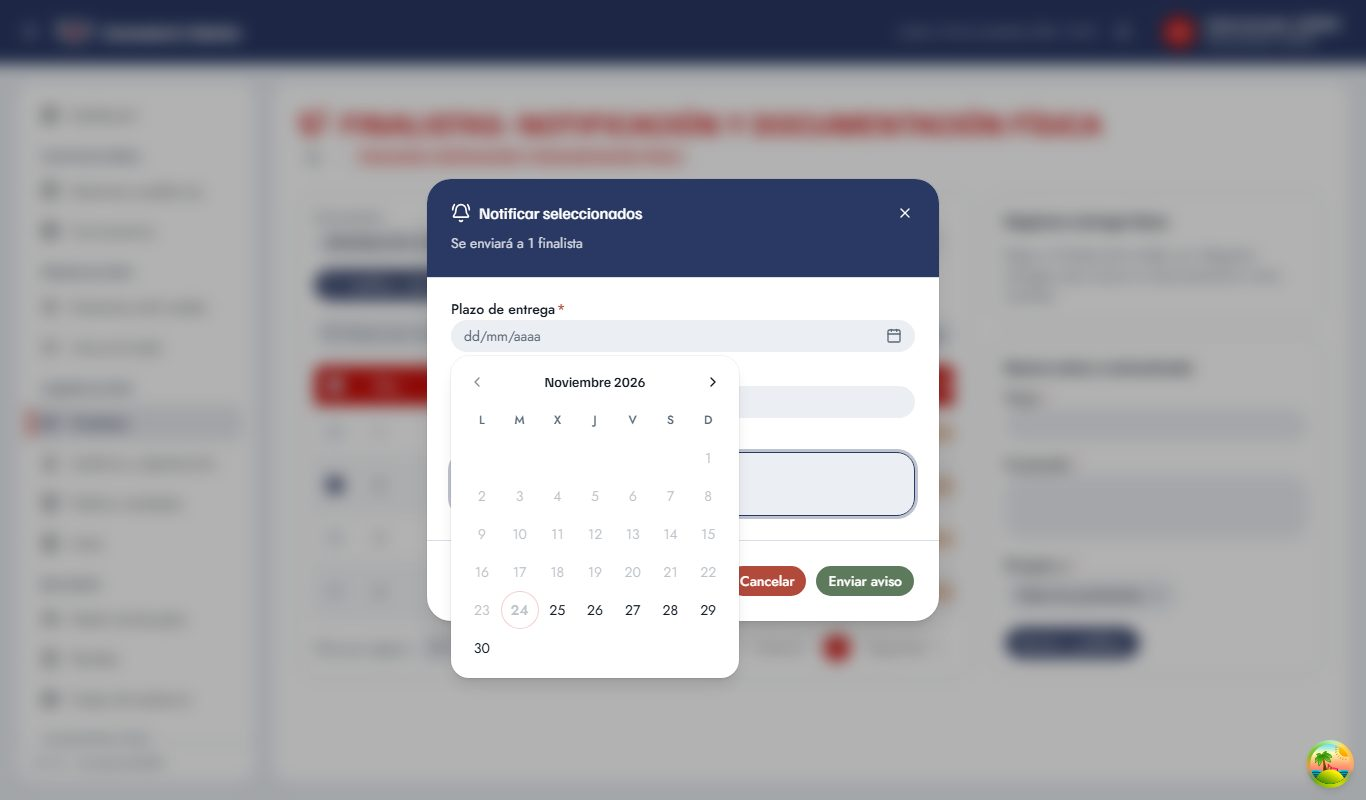
\includegraphics[width=0.93\linewidth,height=4.8cm,keepaspectratio]{images/232_CN_CU-21_B_inicial.jpg}}\vspace{2pt}\end{minipage}} \\
Pasos & {1. Marcar a Ana Zambrana y pulsar «Notificar seleccionados».\newline 2. Abrir el calendario del plazo e intentar elegir el 1 de noviembre.\newline 3. Completar lugar y documentos y pulsar «Enviar aviso».} \\
Resultado esperado & {No se puede elegir una fecha pasada y el envío se bloquea mostrando que el plazo es obligatorio.} \\
Resultado obtenido & {El calendario no permitió elegir el día pasado (día deshabilitado) y al enviar apareció «El plazo de entrega es obligatorio»; no se envió el aviso.} \\
Captura de imagen final & {\begin{minipage}[t]{\linewidth}\strut\par\vspace{3pt}\fcolorbox{gray}{white}{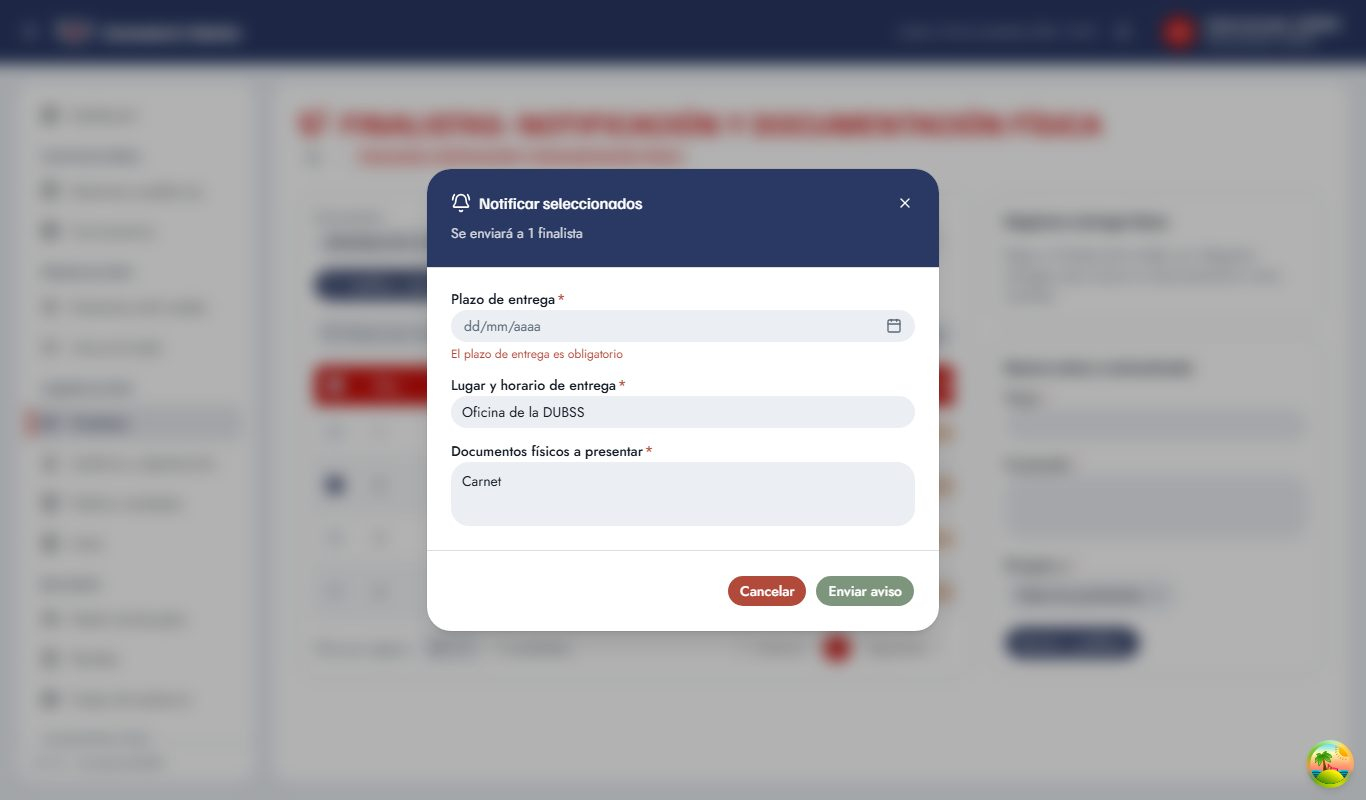
\includegraphics[width=0.93\linewidth,height=4.8cm,keepaspectratio]{images/233_CN_CU-21_B_final.jpg}}\vspace{2pt}\end{minipage}} \\
Resultado de prueba & {\textcolor{green!45!black}{\textbf{CORRECTO}}} \\
\end{longtable}
\endgroup
\addtocounter{table}{-1}
\vspace{-0.5\baselineskip}

\refstepcounter{table}\label{tab:cn_cu21_c}
\addcontentsline{lot}{table}{\protect\numberline{\thetable}CU-21. Notificar finalistas y publicar comunicados (comunicado)}
\noindent\textbf{Tabla~\thetable}\par\nopagebreak
\noindent\textit{CU-21. Notificar finalistas y publicar comunicados (comunicado)}\par\nopagebreak
\begingroup\footnotesize\linespread{1}\selectfont
\setlength{\LTleft}{0pt}\setlength{\LTright}{\fill}
\begin{longtable}{>{\raggedright\arraybackslash}p{3.6cm} >{\raggedright\arraybackslash}p{11.4cm}}
\toprule
\textbf{Campo} & \textbf{Contenido} \\
\midrule
\endfirsthead
\toprule
\textbf{Campo} & \textbf{Contenido} \\
\midrule
\endhead
\midrule
\multicolumn{2}{r}{\textit{Continúa en la siguiente página}} \\
\endfoot
\bottomrule
\multicolumn{2}{l}{\textit{Nota.} Elaboración propia a partir de la ejecución de la prueba.} \\
\endlastfoot
Nombre del caso de prueba & {CU-21. Notificar finalistas y publicar comunicados (comunicado)} \\
Descripción & {El administrador redacta un comunicado, revisa y lo publica a un grupo de destinatarios.} \\
Precondición & {Convocatoria E03 seleccionada (4 finalistas).} \\
Datos de entrada & {Título «Recordatorio de entrega de documentos», contenido «Recuerde presentar su documentación física antes del plazo indicado.», destinatarios «finalistas».} \\
Condición de ejecución & {No aplica} \\
Captura de imagen inicial & {\begin{minipage}[t]{\linewidth}\strut\par\vspace{3pt}\fcolorbox{gray}{white}{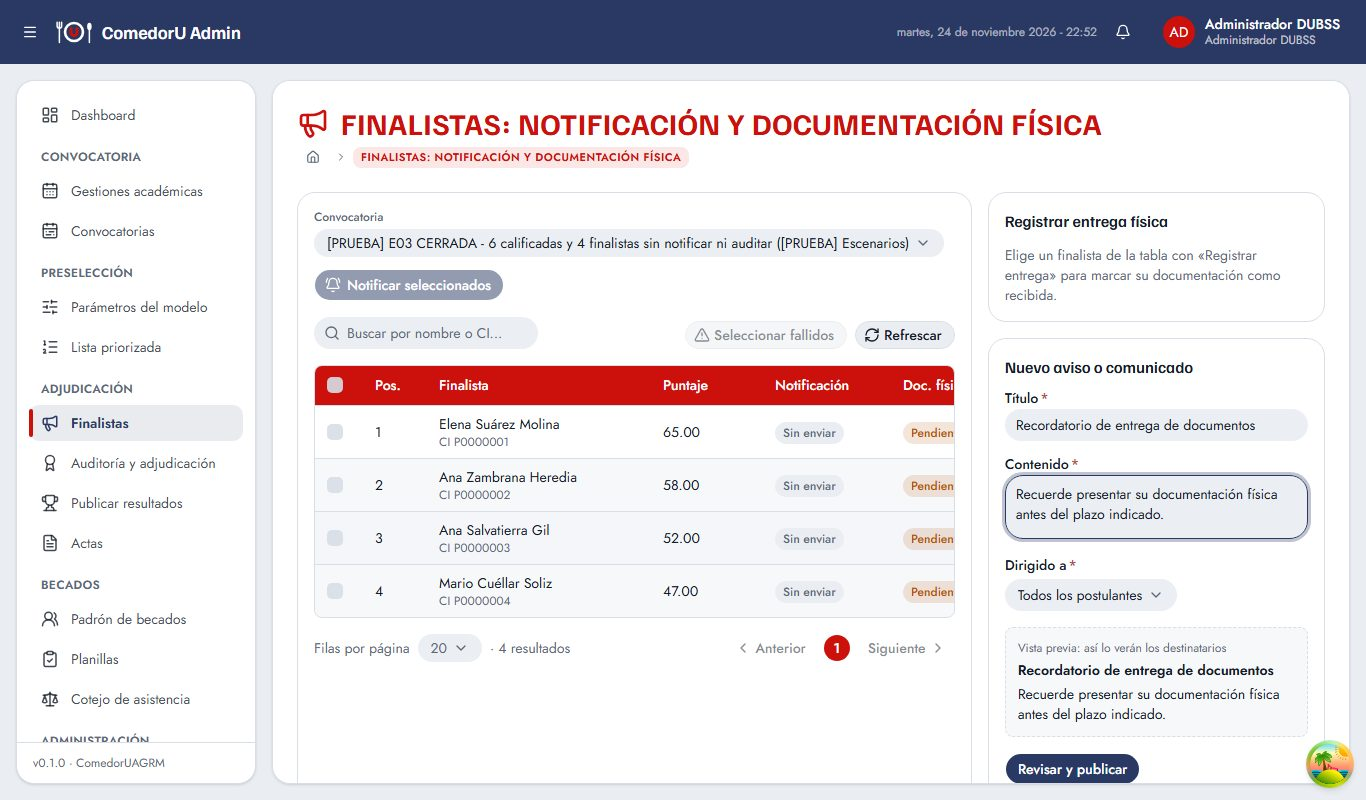
\includegraphics[width=0.93\linewidth,height=4.8cm,keepaspectratio]{images/234_CN_CU-21_C_inicial.jpg}}\vspace{2pt}\end{minipage}} \\
Pasos & {1. En «Nuevo aviso o comunicado» escribir el título y el contenido y elegir «finalistas».\newline 2. Pulsar «Revisar y publicar» y revisar la vista previa.\newline 3. Pulsar «Confirmar publicación».} \\
Resultado esperado & {El comunicado se publica y se informa a cuántos destinatarios llegó.} \\
Resultado obtenido & {La ventana preguntó «¿Publicar el comunicado? Se enviará a finalistas y no podrás editarlo ni borrarlo después.» y el resultado fue «Se envió a 4 destinatarios.».} \\
Captura de imagen final & {\begin{minipage}[t]{\linewidth}\strut\par\vspace{3pt}\fcolorbox{gray}{white}{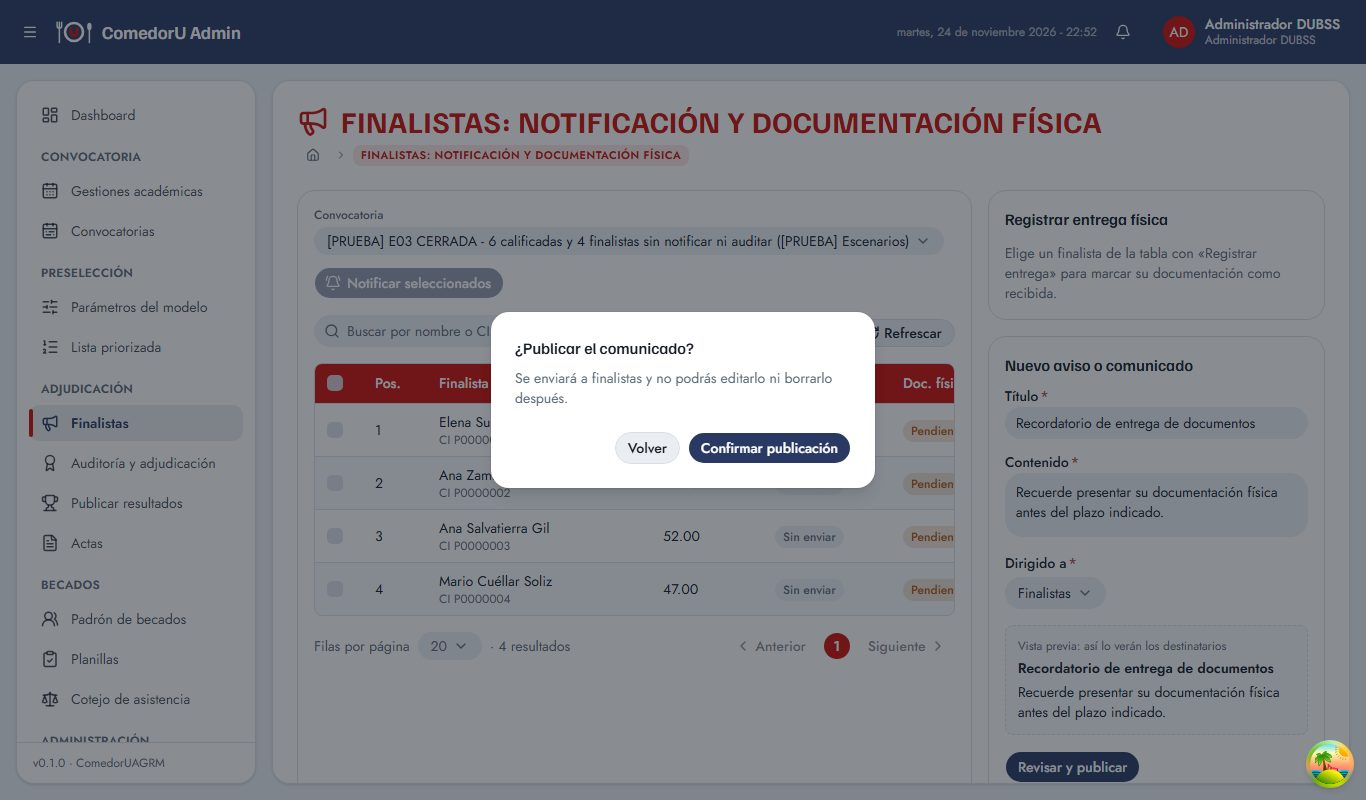
\includegraphics[width=0.93\linewidth,height=4.8cm,keepaspectratio]{images/235_CN_CU-21_C_vista_previa.jpg}}\vspace{2pt}\par\vspace{3pt}\fcolorbox{gray}{white}{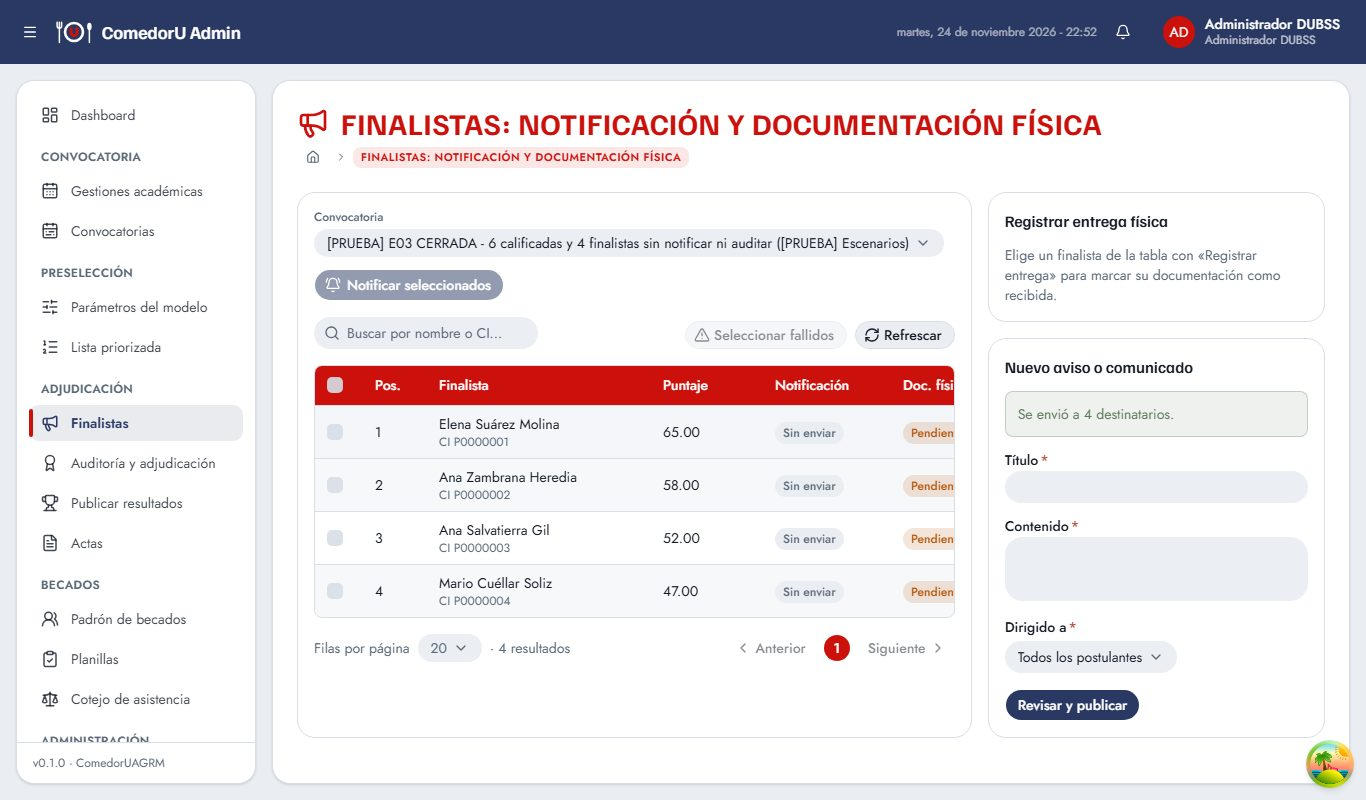
\includegraphics[width=0.93\linewidth,height=4.8cm,keepaspectratio]{images/236_CN_CU-21_C_final.jpg}}\vspace{2pt}\end{minipage}} \\
Resultado de prueba & {\textcolor{green!45!black}{\textbf{CORRECTO}}} \\
\end{longtable}
\endgroup
\addtocounter{table}{-1}
\vspace{-0.5\baselineskip}

\refstepcounter{table}\label{tab:cn_cu21_d}
\addcontentsline{lot}{table}{\protect\numberline{\thetable}CU-21. Notificar finalistas y publicar comunicados (sin destinatarios)}
\noindent\textbf{Tabla~\thetable}\par\nopagebreak
\noindent\textit{CU-21. Notificar finalistas y publicar comunicados (sin destinatarios)}\par\nopagebreak
\begingroup\footnotesize\linespread{1}\selectfont
\setlength{\LTleft}{0pt}\setlength{\LTright}{\fill}
\begin{longtable}{>{\raggedright\arraybackslash}p{3.6cm} >{\raggedright\arraybackslash}p{11.4cm}}
\toprule
\textbf{Campo} & \textbf{Contenido} \\
\midrule
\endfirsthead
\toprule
\textbf{Campo} & \textbf{Contenido} \\
\midrule
\endhead
\midrule
\multicolumn{2}{r}{\textit{Continúa en la siguiente página}} \\
\endfoot
\bottomrule
\multicolumn{2}{l}{\textit{Nota.} Elaboración propia a partir de la ejecución de la prueba.} \\
\endlastfoot
Nombre del caso de prueba & {CU-21. Notificar finalistas y publicar comunicados (sin destinatarios)} \\
Descripción & {El sistema avisa cuando el grupo elegido no tiene destinatarios.} \\
Precondición & {Convocatoria seleccionada por defecto «[PRUEBA] Convocatoria sin postulaciones» (sin finalistas).} \\
Datos de entrada & {Título y contenido de prueba, destinatarios «finalistas».} \\
Condición de ejecución & {No aplica} \\
Captura de imagen inicial & {\begin{minipage}[t]{\linewidth}\strut\par\vspace{3pt}\fcolorbox{gray}{white}{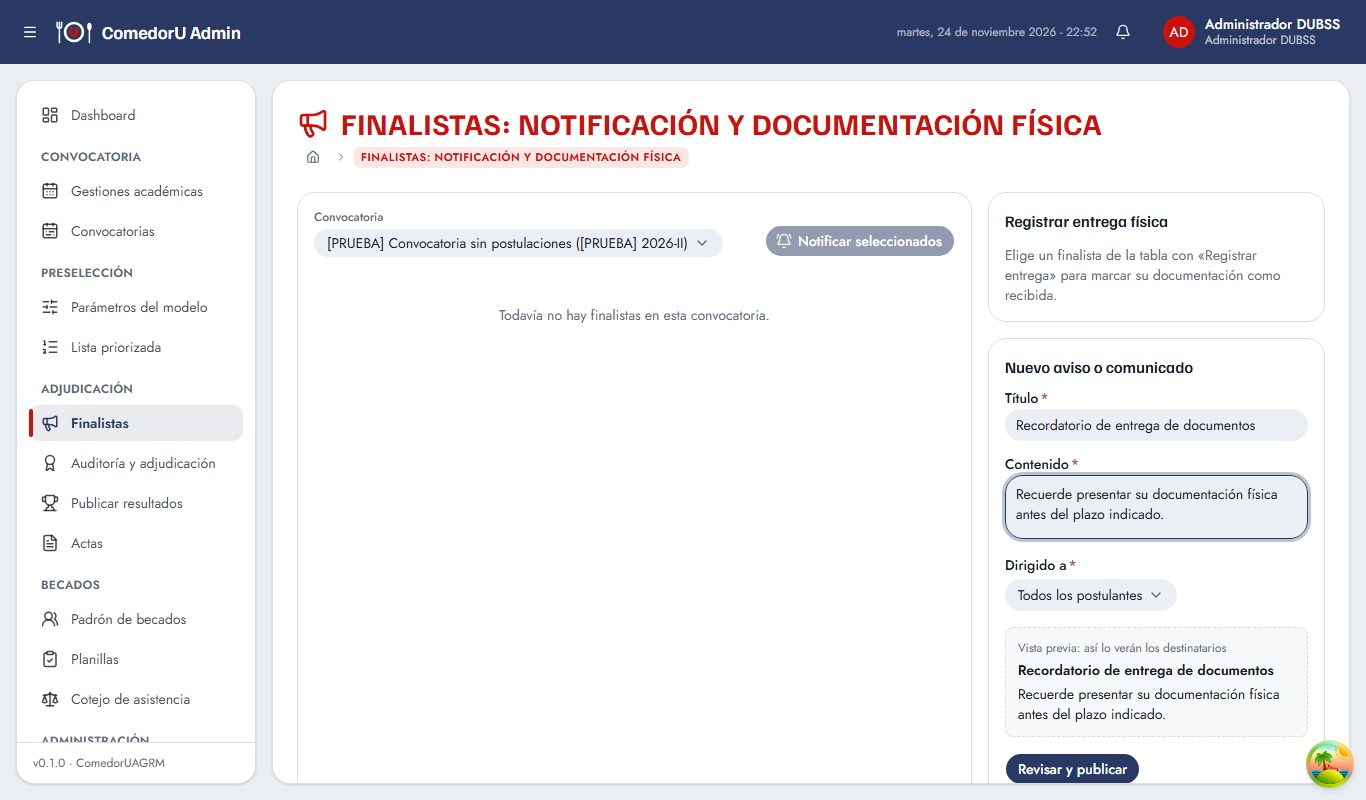
\includegraphics[width=0.93\linewidth,height=4.8cm,keepaspectratio]{images/237_CN_CU-21_D_inicial.jpg}}\vspace{2pt}\end{minipage}} \\
Pasos & {1. Escribir título y contenido y elegir «finalistas».\newline 2. Pulsar «Revisar y publicar» y luego «Confirmar publicación».} \\
Resultado esperado & {No se publica y se informa que no hay destinatarios.} \\
Resultado obtenido & {Se mostró «No hay destinatarios para ese comunicado.».} \\
Captura de imagen final & {\begin{minipage}[t]{\linewidth}\strut\par\vspace{3pt}\fcolorbox{gray}{white}{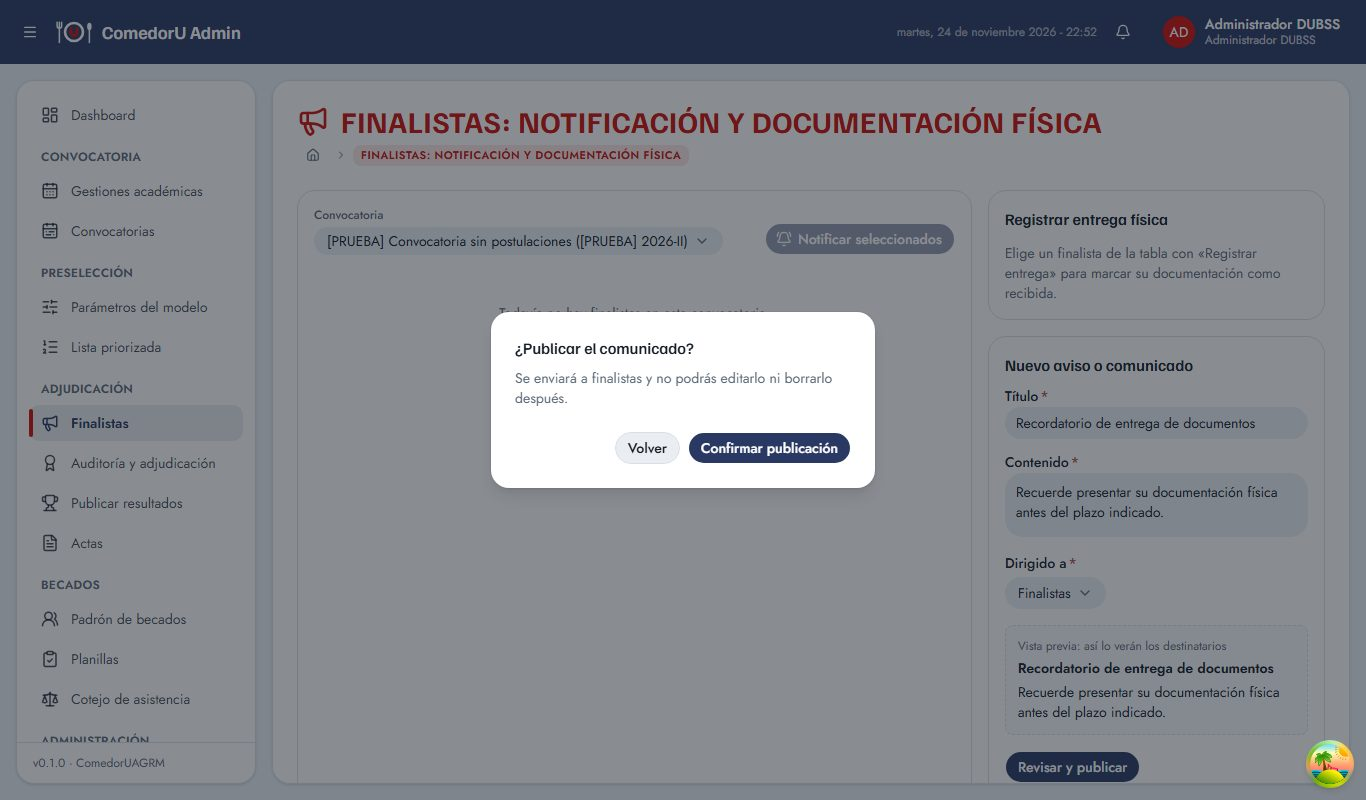
\includegraphics[width=0.93\linewidth,height=4.8cm,keepaspectratio]{images/238_CN_CU-21_D_vista_previa.jpg}}\vspace{2pt}\par\vspace{3pt}\fcolorbox{gray}{white}{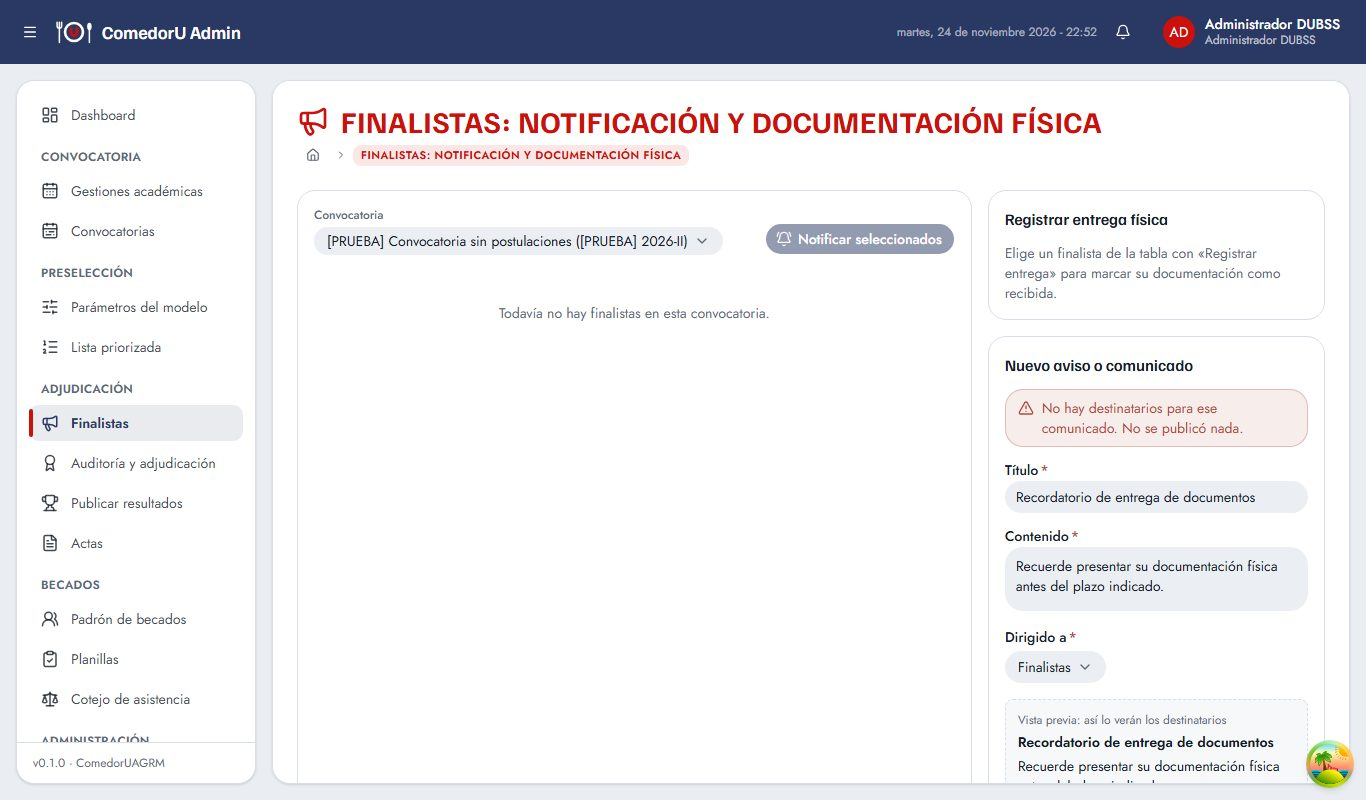
\includegraphics[width=0.93\linewidth,height=4.8cm,keepaspectratio]{images/239_CN_CU-21_D_final.jpg}}\vspace{2pt}\end{minipage}} \\
Resultado de prueba & {\textcolor{green!45!black}{\textbf{CORRECTO}}} \\
\end{longtable}
\endgroup
\addtocounter{table}{-1}
\vspace{-0.5\baselineskip}

\paragraph{CU-22. Publicar resultados de adjudicación.}\label{sec:cn_cu22} 

\refstepcounter{table}\label{tab:cn_cu22_a}
\addcontentsline{lot}{table}{\protect\numberline{\thetable}CU-22. Publicar resultados de adjudicación (publicación)}
\noindent\textbf{Tabla~\thetable}\par\nopagebreak
\noindent\textit{CU-22. Publicar resultados de adjudicación (publicación)}\par\nopagebreak
\begingroup\footnotesize\linespread{1}\selectfont
\setlength{\LTleft}{0pt}\setlength{\LTright}{\fill}
\begin{longtable}{>{\raggedright\arraybackslash}p{3.6cm} >{\raggedright\arraybackslash}p{11.4cm}}
\toprule
\textbf{Campo} & \textbf{Contenido} \\
\midrule
\endfirsthead
\toprule
\textbf{Campo} & \textbf{Contenido} \\
\midrule
\endhead
\midrule
\multicolumn{2}{r}{\textit{Continúa en la siguiente página}} \\
\endfoot
\bottomrule
\multicolumn{2}{l}{\textit{Nota.} Elaboración propia a partir de la ejecución de la prueba.} \\
\endlastfoot
Nombre del caso de prueba & {CU-22. Publicar resultados de adjudicación (publicación)} \\
Descripción & {El administrador publica las decisiones de una convocatoria cerrada y se avisa a los finalistas.} \\
Precondición & {Convocatoria sembrada «[PRUEBA] E05»: cerrada, 2 adjudicados, 1 no adjudicado, sin decisiones pendientes.} \\
Datos de entrada & {Convocatoria E05.} \\
Condición de ejecución & {La convocatoria debe estar cerrada y sin decisiones pendientes; la publicación no se puede deshacer.} \\
Captura de imagen inicial & {\begin{minipage}[t]{\linewidth}\strut\par\vspace{3pt}\fcolorbox{gray}{white}{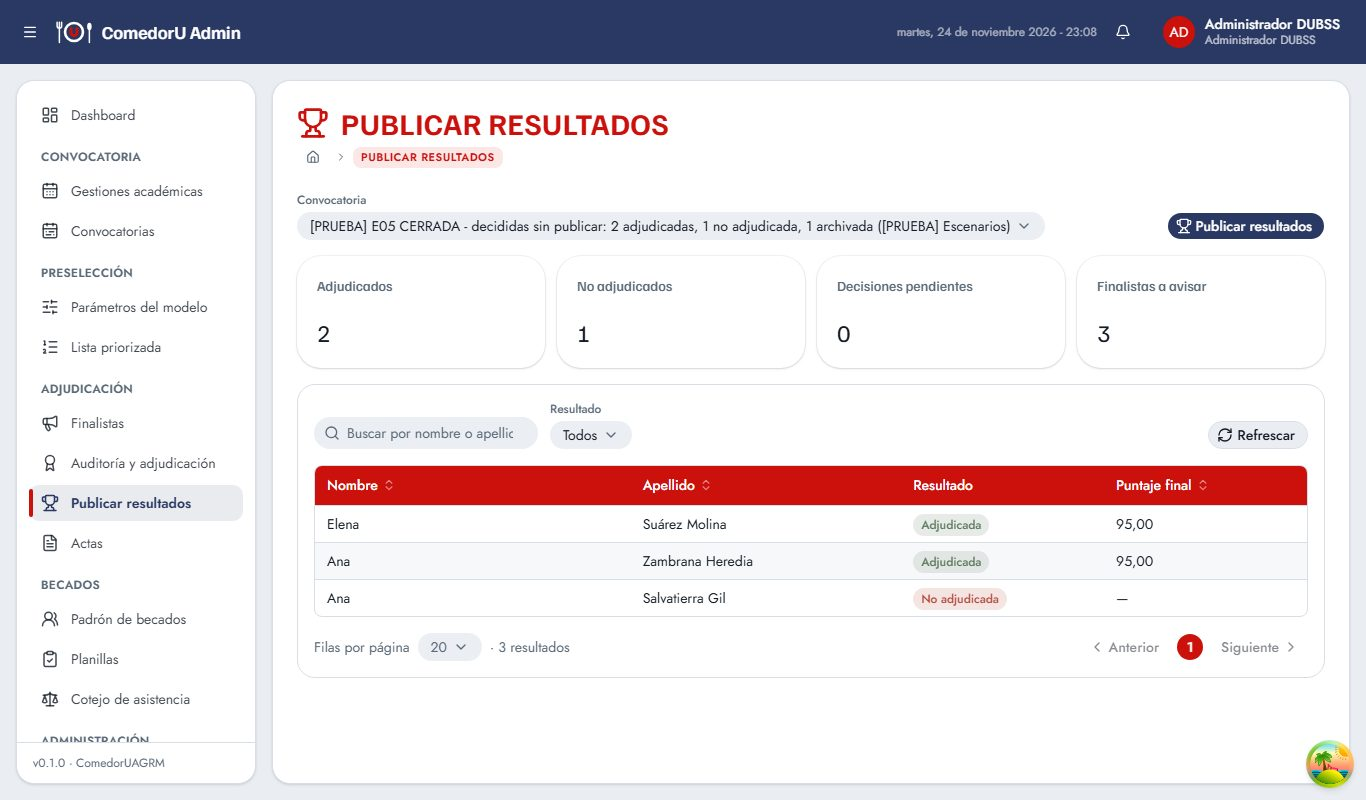
\includegraphics[width=0.93\linewidth,height=4.8cm,keepaspectratio]{images/240_CN_CU-22_A_inicial.jpg}}\vspace{2pt}\end{minipage}} \\
Pasos & {1. Abrir «Publicar resultados» y elegir E05.\newline 2. Pulsar «Publicar resultados».\newline 3. Confirmar con «Publicar» en la ventana.} \\
Resultado esperado & {Se publican los resultados y se envía un aviso a cada finalista con decisión.} \\
Resultado obtenido & {La ventana indicó «hay 2 adjudicados y 1 no adjudicados. Se avisará a 3 finalistas…». Tras publicar apareció «publicados el 24/11/2026, 11:08 p. m.» y Mailpit recibió tres correos «Beca Comedor: resultado de tu postulación» (postulante.0000001, 0000002 y 0000003).} \\
Captura de imagen final & {\begin{minipage}[t]{\linewidth}\strut\par\vspace{3pt}\fcolorbox{gray}{white}{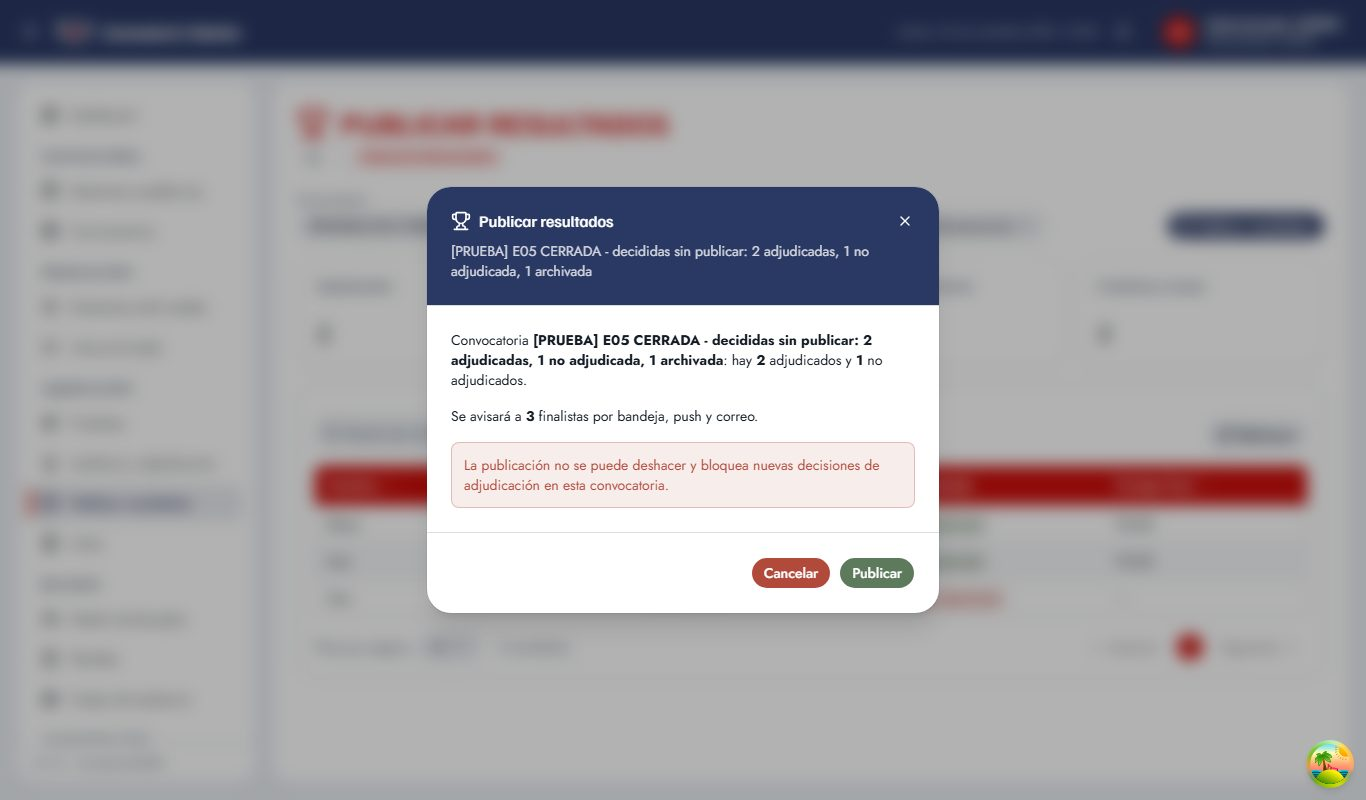
\includegraphics[width=0.93\linewidth,height=4.8cm,keepaspectratio]{images/241_CN_CU-22_A_confirmacion.jpg}}\vspace{2pt}\par\vspace{3pt}\fcolorbox{gray}{white}{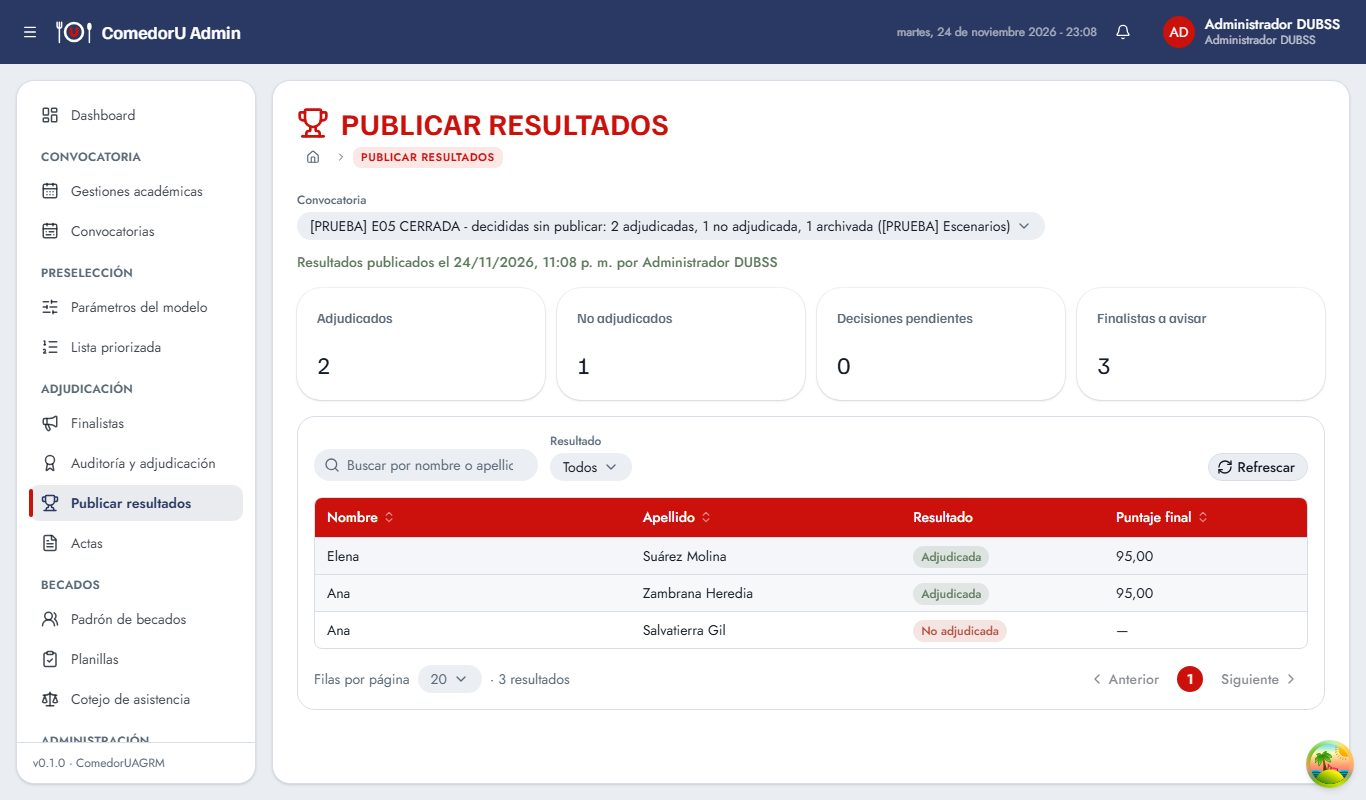
\includegraphics[width=0.93\linewidth,height=4.8cm,keepaspectratio]{images/242_CN_CU-22_A_final.jpg}}\vspace{2pt}\end{minipage}} \\
Resultado de prueba & {\textcolor{green!45!black}{\textbf{CORRECTO}}} \\
\end{longtable}
\endgroup
\addtocounter{table}{-1}
\vspace{-0.5\baselineskip}

\refstepcounter{table}\label{tab:cn_cu22_b}
\addcontentsline{lot}{table}{\protect\numberline{\thetable}CU-22. Publicar resultados de adjudicación (decisiones pendientes)}
\noindent\textbf{Tabla~\thetable}\par\nopagebreak
\noindent\textit{CU-22. Publicar resultados de adjudicación (decisiones pendientes)}\par\nopagebreak
\begingroup\footnotesize\linespread{1}\selectfont
\setlength{\LTleft}{0pt}\setlength{\LTright}{\fill}
\begin{longtable}{>{\raggedright\arraybackslash}p{3.6cm} >{\raggedright\arraybackslash}p{11.4cm}}
\toprule
\textbf{Campo} & \textbf{Contenido} \\
\midrule
\endfirsthead
\toprule
\textbf{Campo} & \textbf{Contenido} \\
\midrule
\endhead
\midrule
\multicolumn{2}{r}{\textit{Continúa en la siguiente página}} \\
\endfoot
\bottomrule
\multicolumn{2}{l}{\textit{Nota.} Elaboración propia a partir de la ejecución de la prueba.} \\
\endlastfoot
Nombre del caso de prueba & {CU-22. Publicar resultados de adjudicación (decisiones pendientes)} \\
Descripción & {No se publica una convocatoria con finalistas sin decidir.} \\
Precondición & {Convocatoria «[PRUEBA] Con pendientes» con 1 finalista sin decisión.} \\
Datos de entrada & {Convocatoria «Con pendientes».} \\
Condición de ejecución & {No aplica} \\
Captura de imagen inicial & {\begin{minipage}[t]{\linewidth}\strut\par\vspace{3pt}\fcolorbox{gray}{white}{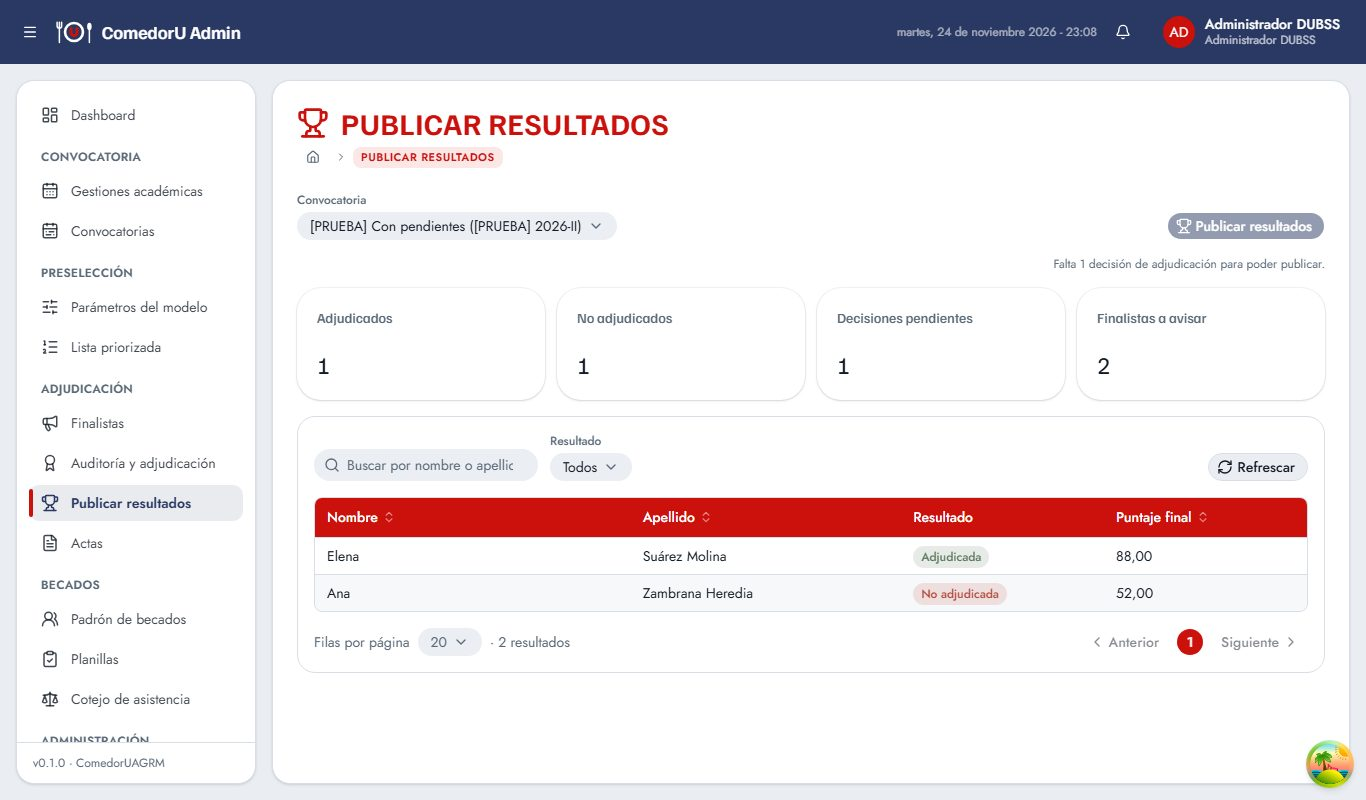
\includegraphics[width=0.93\linewidth,height=4.8cm,keepaspectratio]{images/243_CN_CU-22_B_inicial.jpg}}\vspace{2pt}\end{minipage}} \\
Pasos & {1. Abrir «Publicar resultados» y elegir «Con pendientes».\newline 2. Intentar pulsar «Publicar resultados».} \\
Resultado esperado & {El botón está deshabilitado y se indica cuántas decisiones faltan.} \\
Resultado obtenido & {Se mostró «Falta 1 decisión de adjudicación para poder publicar.» y el botón estaba deshabilitado.} \\
Captura de imagen final & {\begin{minipage}[t]{\linewidth}\strut\par\vspace{3pt}\fcolorbox{gray}{white}{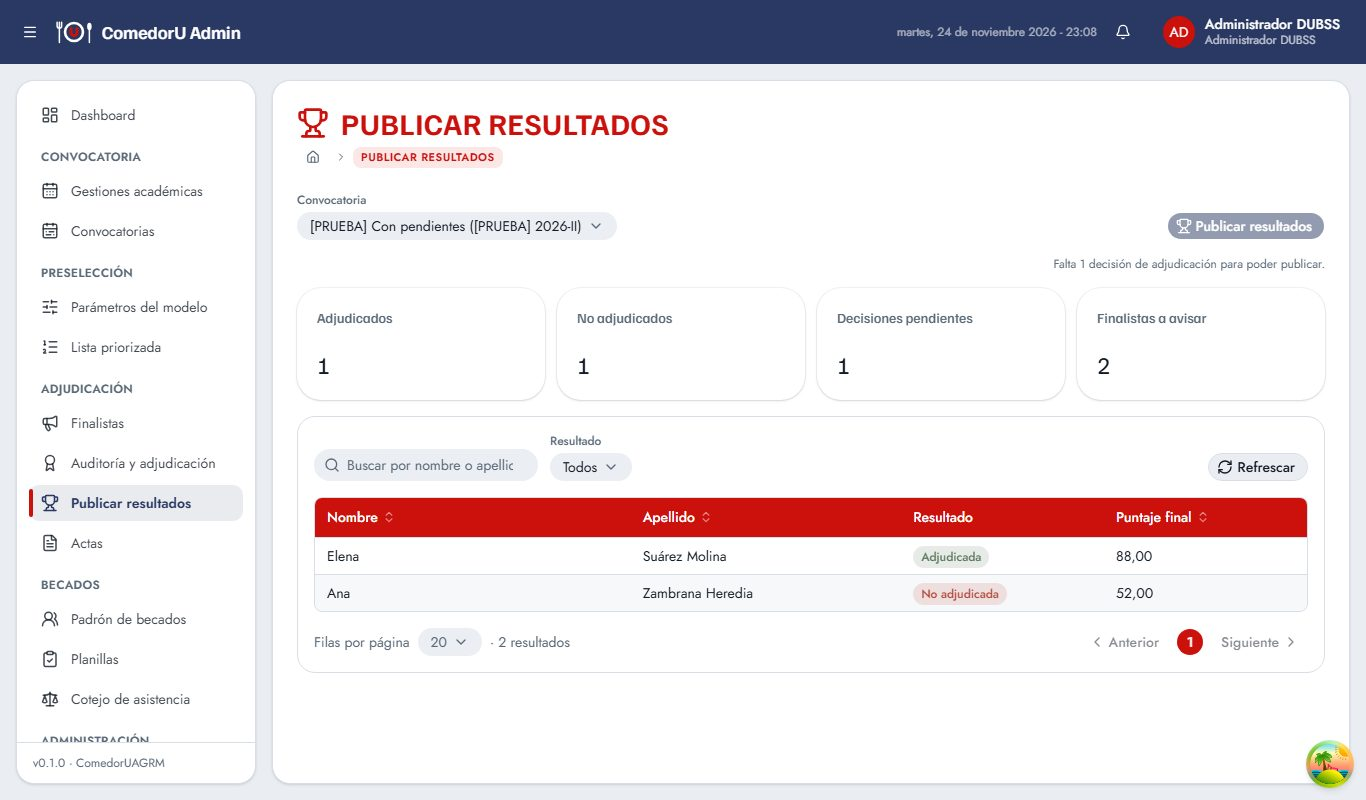
\includegraphics[width=0.93\linewidth,height=4.8cm,keepaspectratio]{images/244_CN_CU-22_B_final.jpg}}\vspace{2pt}\end{minipage}} \\
Resultado de prueba & {\textcolor{green!45!black}{\textbf{CORRECTO}}} \\
\end{longtable}
\endgroup
\addtocounter{table}{-1}
\vspace{-0.5\baselineskip}

\refstepcounter{table}\label{tab:cn_cu22_c}
\addcontentsline{lot}{table}{\protect\numberline{\thetable}CU-22. Publicar resultados de adjudicación (consulta del postulante)}
\noindent\textbf{Tabla~\thetable}\par\nopagebreak
\noindent\textit{CU-22. Publicar resultados de adjudicación (consulta del postulante)}\par\nopagebreak
\begingroup\footnotesize\linespread{1}\selectfont
\setlength{\LTleft}{0pt}\setlength{\LTright}{\fill}
\begin{longtable}{>{\raggedright\arraybackslash}p{3.6cm} >{\raggedright\arraybackslash}p{11.4cm}}
\toprule
\textbf{Campo} & \textbf{Contenido} \\
\midrule
\endfirsthead
\toprule
\textbf{Campo} & \textbf{Contenido} \\
\midrule
\endhead
\midrule
\multicolumn{2}{r}{\textit{Continúa en la siguiente página}} \\
\endfoot
\bottomrule
\multicolumn{2}{l}{\textit{Nota.} Elaboración propia a partir de la ejecución de la prueba.} \\
\endlastfoot
Nombre del caso de prueba & {CU-22. Publicar resultados de adjudicación (consulta del postulante)} \\
Descripción & {El postulante ve la lista pública de adjudicados de las convocatorias publicadas.} \\
Precondición & {Sesión de \texttt{postulante.\allowbreak{}finalista@\allowbreak{}prueba.\allowbreak{}local}; E05 recién publicada.} \\
Datos de entrada & {Convocatorias E05 y E06.} \\
Condición de ejecución & {No aplica} \\
Captura de imagen inicial & {\begin{minipage}[t]{\linewidth}\strut\par\vspace{3pt}\fcolorbox{gray}{white}{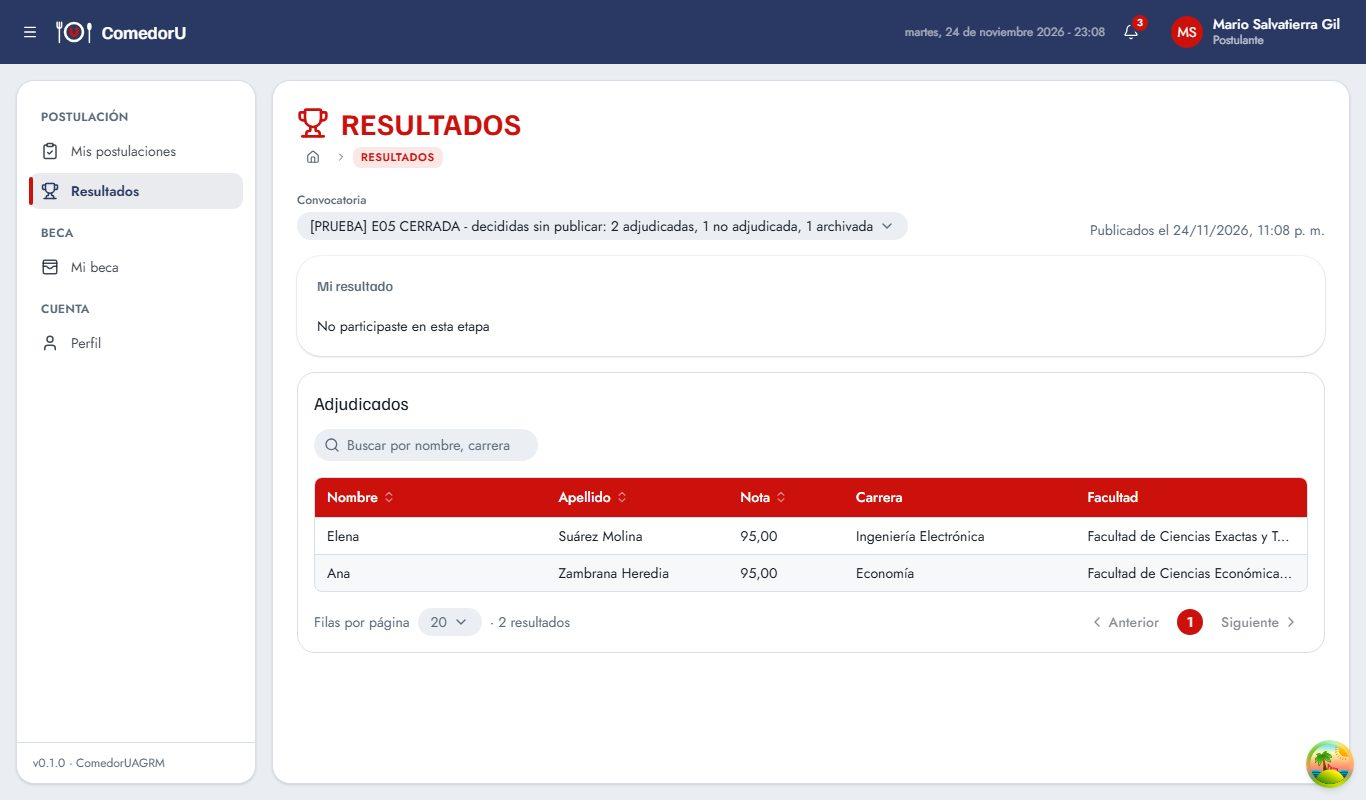
\includegraphics[width=0.93\linewidth,height=4.8cm,keepaspectratio]{images/245_CN_CU-22_C_inicial.jpg}}\vspace{2pt}\end{minipage}} \\
Pasos & {1. Abrir \texttt{/\allowbreak{}resultados}.\newline 2. Revisar la convocatoria E05 y elegir la E06.} \\
Resultado esperado & {Se muestran fecha de publicación, «Mi resultado» y la lista de adjudicados con nombre, nota, carrera y facultad (sin motivos de decisión).} \\
Resultado obtenido & {E05 mostró «Publicados el 24/11/2026», «Mi resultado: No participaste en esta etapa» y 2 adjudicados con nota 95,00, carrera y facultad. E06 mostró 3 adjudicados.} \\
Captura de imagen final & {\begin{minipage}[t]{\linewidth}\strut\par\vspace{3pt}\fcolorbox{gray}{white}{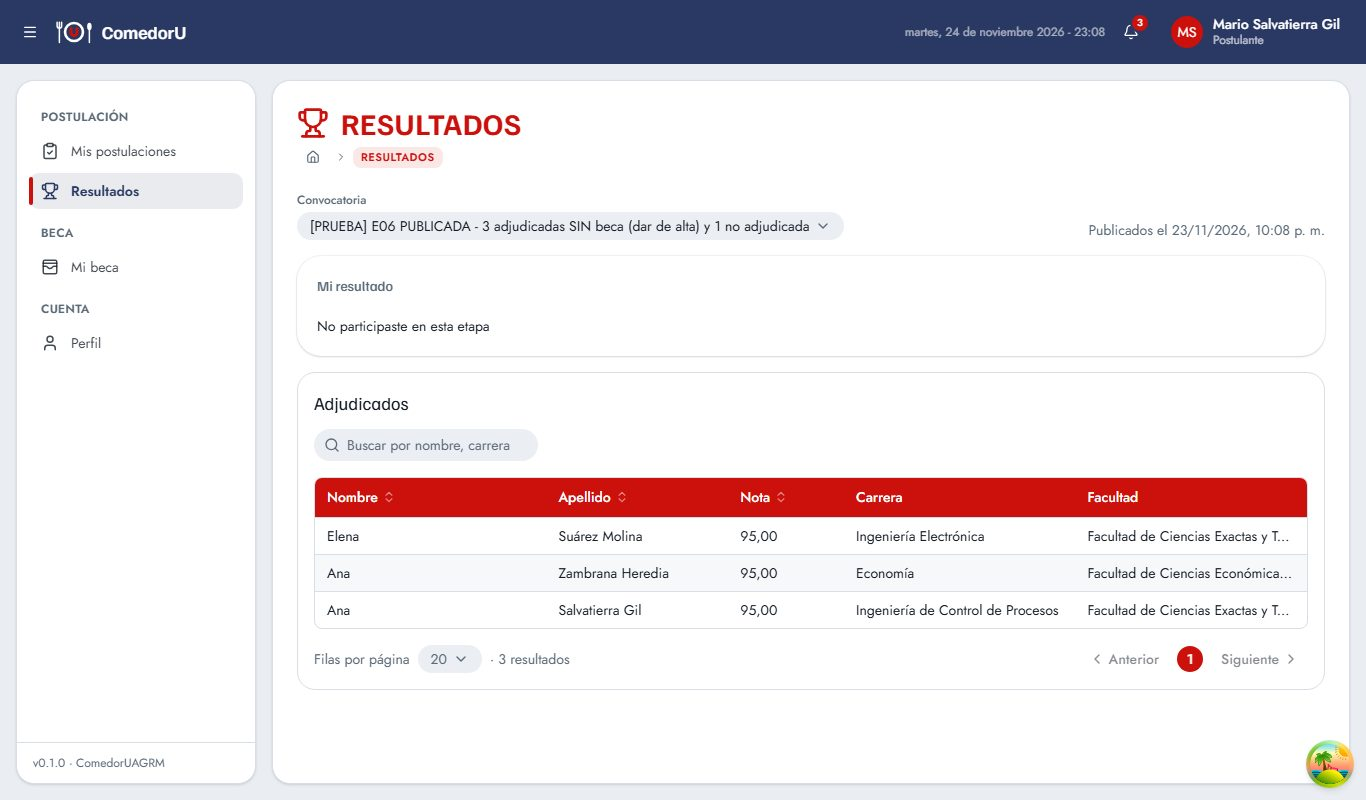
\includegraphics[width=0.93\linewidth,height=4.8cm,keepaspectratio]{images/246_CN_CU-22_C_final.jpg}}\vspace{2pt}\end{minipage}} \\
Resultado de prueba & {\textcolor{green!45!black}{\textbf{CORRECTO}}} \\
\end{longtable}
\endgroup
\addtocounter{table}{-1}
\vspace{-0.5\baselineskip}
